\def \rootFolder{../}

% this has all the necessary packages and formatting for the document
\documentclass[10pt,a5paper,landscape]{article}

%packages
\usepackage[left=1cm,right=1cm,top=1cm,bottom=1cm]{geometry}

\usepackage[chorded]{\rootFolder/_include/psalterio} %must check the licence to change the name of the sty file!!!
%\usepackage[chorded]{resources/songs-old} %must check the licence to change the name of the sty file!!!

\usepackage[utf8]{inputenc}
%\usepackage[utf8,latin1]{inputenc}

\usepackage{graphicx}
\usepackage{wrapfig}
\usepackage{wallpaper}
\usepackage{color}
\usepackage{eso-pic} %for background pictures
\usepackage[bookmarks]{hyperref} 
%\usepackage{ifthen} %etoolbox is more up to date
\usepackage{etoolbox}

%\usepackage[xetex]{graphicx}
%\usepackage{fontspec,xunicode}
%\defaultfontfeatures{Mapping=tex-text,Scale=MatchLowercase}
%\setmainfont[Scale=.95]{Times}
%\setmonofont{Lucida Sans Typewriter}

%\usepackage[portuguese]{babel}
%\usepackage[latin1]{inputenc}
%\usepackage[utf8]{inputenc}
%\usepackage[T1]{fontenc}
%\usepackage[scaled]{uarial}
%\usepackage{helvet}
%\renewcommand{\familydefault}{\sfdefault}

%this removes the page number
\thispagestyle{empty}
\pagestyle{empty}
\songcolumns{2}

\parindent 0pt	


%add background picture
\newcommand\BackgroundPic{
\put(0,0){
\parbox[b][\paperheight]{\paperwidth}{%
\vfill
\centering

\includegraphics[width=\paperwidth,height=\paperheight,
keepaspectratio]{logo.png}%
\vfill
}}}

\newcommand\BottomPic{
\put(0,0){
\includegraphics{\rootFolder/_images/bkground_page_bottom.png}
}}




%
%Font Sizes
%
%\tiny
%\scriptsize
%\footnotesize
%\small
%\normalsize
%\large
%\Large
%\LARGE
%\huge
%\Huge

%%% format song number
%\renewcommand{\thesongnum}{A\arabic{songnum}}
\renewcommand{\printsongnum}[1]{\sffamily\bfseries\huge\MakeUppercase#1}
\setlength{\songnumwidth}{1.5cm} % box width
%\renewcommand{\snumbgcolor}{white}

%%% format title
%change font for Title
%\renewcommand{\stitlefont}{\sffamily\bfseries\huge\MakeUppercase} 
\renewcommand{\stitlefont}{\sffamily\bfseries\huge}
%song title

%%% format verse numbers
%remove verse numbers
%\noversenumbers 
% make left separation
\setlength{\versenumwidth}{.5cm}


%verse separations
%\versesep=15pt
%\afterpreludeskip=2pt
%\beforepostludeskip=2pt
%\baselineadj=10pt

% separation between chords and lyrics
\renewcommand{\clineparams}{ 
\baselineskip=11pt 
%\lineskiplimit=2pt 
%\lineskip=5pt
}

%\setlength{\oddsidemargin}{0in}
%\setlength{\evensidemargin}{0in}

% change font for lyrics
%\renewcommand{\lyricfont}{\sffamily}
%\renewcommand{\lyricfont}{\sffamily\small}
\renewcommand{\lyricfont}{\sffamily\large}
%\renewcommand{\chorusfont}{\sffamily}
\renewcommand{\chorusfont}{\sffamily\large}

%change the Chords formatting
\renewcommand{\printchord}[1]{\sffamily\color{red}\it\normalsize#1}

%check http://www.tug.org/pracjourn/2006-1/schmidt/schmidt.pdf


%\renewcommand{\songauthors}[1]{tete #1}


%\renewcommand{\extendpostlude}
%{ \songcopyright\ \songlicense\unskip \ Used with permission.}

% chorus bar width
\setlength{\cbarwidth}{0pt}

%\renewcommand{\chorusjustify}{\justifyleft}


\setlength{\sbarheight}{0pt}

% music anf lyrics by
\newcommand{\musicLyricsBy}{} 
\newsongkey{mlby}{\def\musicLyricsBy{}}
                 {\def\musicLyricsBy{\sffamily\it\small letra e música por #1\par}}

% music by
\newcommand{\musicby}{} 
\newsongkey{musicby}{\def\musicby{}}
                 {\def\musicby{\sffamily\it\small música por #1\par}}

% lyrics by
\newcommand{\lyricsby}{} 
\newsongkey{lyricsby}{\def\lyricsby{}}
                 {\def\lyricsby{\sffamily\it\small letra por #1\par}}

% number
\newcommand{\psalterionumber}{} 
\newsongkey{psalterionumber}{\def\psalterionumber{}}
                 {\def\psalterionumber{\sffamily\it\small Psaltério #1\par}}


%\renewcommand{\sharpsymbol}{\ensuremath{^\sharp}}
\renewcommand{\extendprelude}{
  \showrefs\showauthors 
  {\bfseries\musicLyricsBy}
  {\bfseries\musicby}
  {\bfseries\lyricsby}
}

\def \gtabsOn{1}

% this includes all the guitar tabs that may be needed
%% must complete all the chords used in psalterio

% Cb chords

% C chords
\def \gtabCb{\gtab{Cb}{X32010:X32010}}
\def \gtabC{\gtab{C}{X32010:032010}}
\def \gtabCm{\gtab{Cm}{3:113321:004320}}

\def \gtabCsharpSusFour{\gtab{C\#sus4}{4:XX3341:XX2341}}

% Db chords

% D chords
\def \gtabD{\gtab{D}{X00232:000132}}
\def \gtabDm{\gtab{Dm}{X00231:000231}}
\def \gtabDfour{\gtab{D4}{X00233:000134}}
\def \gtabDseven{\gtab{D7}{X00212:000213}}
\def \gtabDsevenPlus{\gtab{D7+}{X00222:000111}}

% D#/Eb chords
\def \gtabDsharp{\gtab{D\#}{2:XX0232:000132}}

% E chords
\def \gtabE{\gtab{E}{022100:023100}}
\def \gtabEseven{\gtab{E}{020100:020100}}

\def \gtabEm{\gtab{Em}{022000:012000}}
\def \gtabEmSeven{\gtab{Em7}{022030:012040}}

% Gb chords

% F chords
\def \gtabF{\gtab{F}{1:133211:034200}}
\def \gtabFm{\gtab{Fm}{1:133111:034000}}


% F# chords
\def \gtabFsharpMinor{\gtab{F\#m}{2:133111:034000}}
\def \gtabFsharpMinorSeven{\gtab{F\#m7}{2:131131:030040}}

% Gb chords

% G chords
\def \gtabG{\gtab{G}{320033:210034}}
\def \gtabGseven{\gtab{G7}{320001:320001}}
\def \gtabGfret{\gtab{(G)}{3:133211:034200}}
\def \gtabGm{\gtab{Gm}{3:133111:034000}}


% G# / Ab chords

% A chords
\def \gtabA{\gtab{A}{X02220:001230}}
\def \gtabAm{\gtab{Am}{X02210:002310}}
\def \gtabAmSeven{\gtab{Am7}{X02010:002010}}
\def \gtabAfour{\gtab{A4}{X02230:001230}}
\def \gtabAseven{\gtab{A7}{X02020:001030}}

% Bb chords
\def \gtabBb{\gtab{Bb}{X13331}}

% B chords
\def \gtabB{\gtab{B}{X13331:003210}}
\def \gtabBm{\gtab{Bm}{X13321:003420}}
\def \gtabBmSeven{\gtab{Bm7}{X13121:003020}}



% after any { or } at the end of a line inside the macro definition add %, otherwise you'll get an extra space
\newcommand{\guitarTab}[1]{%
\ifstrequal{#1}{Cb}      {\gtab{Cb}{X32010:X32010}      }{}%
\ifstrequal{#1}{C}        { \gtab{C}{X32010:032010}       }{}%
%
%G
%
\ifstrequal{#1}{G}       { \gtab{G}{320033:210034}       }{}%
\ifstrequal{#1}{G7}     { \gtab{G7}{320001:320001}     }{}%
\ifstrequal{#1}{Gfret}  { \gtab{G}{3:133211:034200}    }{}%
\ifstrequal{#1}{Gm}    { \gtab{Gm}{3:133111:034000}  }{}%
} %end \newcommand{\gtab}

\providebool{gchords}
\setbool{gchords}{false}

% set guitar chords vertical space separation with lyrics
\def \gchordsVspace{5 mm}

\begin{document}

	%\showindex{Complete Index of Songs}{titleidx}
	\songsection{} % no title

	\AddToShipoutPicture{\BottomPic}
	
	\begin{songs}{}
	% \begin{songs}{titleidx,authidx,scripidx}
	%\begin{songs}{titleidx}
	
	%%
%Font Sizes
%
%\tiny
%\scriptsize
%\footnotesize
%\small
%\normalsize
%\large
%\Large
%\LARGE
%\huge
%\Huge


%\renewcommand{\thesongnum}{A\arabic{songnum}}
\renewcommand{\printsongnum}[1]{\sffamily\bfseries\huge\MakeUppercase#1}
\setlength{\songnumwidth}{2cm} % box width
%\renewcommand{\snumbgcolor}{white}

%change font for Title
\renewcommand{\stitlefont}{\sffamily\bfseries\huge\MakeUppercase} %song title

%remove verse numbers
%\noversenumbers 
% make left separation
\setlength{\versenumwidth}{2.0cm}

%verse separations
%\versesep=15pt
%\afterpreludeskip=2pt
%\beforepostludeskip=2pt
%\baselineadj=10pt

% separation between chords and lyrics
\renewcommand{\clineparams}{ 
\baselineskip=10pt 
%\lineskiplimit=2pt 
%\lineskip=5pt
}

% change font for lyrics
%\renewcommand{\lyricfont}{\sffamily}
%\renewcommand{\lyricfont}{\sffamily\small}
\renewcommand{\lyricfont}{\sffamily\large}
%\renewcommand{\chorusfont}{\sffamily}
\renewcommand{\chorusfont}{\sffamily\large}

%change the Chords formatting
\renewcommand{\printchord}[1]{\sffamily\color{red}\it\normalsize#1}

%check http://www.tug.org/pracjourn/2006-1/schmidt/schmidt.pdf


%\renewcommand{\songauthors}[1]{tete #1}


%\renewcommand{\extendpostlude}
%{ \songcopyright\ \songlicense\unskip \ Used with permission.}

\setlength{\cbarwidth}{0pt}
\setlength{\sbarheight}{0pt}

% music anf lyrics by
\newcommand{\musicLyricsBy}{} 
\newsongkey{mlby}{\def\musicLyricsBy{}}
                 {\def\musicLyricsBy{\sffamily\it\small letra e música por #1\par}}

% music anf lyrics by
\newcommand{\musicby}{} 
\newsongkey{music}{\def\musicby{}}
                 {\def\musicby{\sffamily\it\small música: #1\par}}

% music anf lyrics by
\newcommand{\lyricsby}{} 
\newsongkey{lyrics}{\def\lyricsby{}}
                 {\def\lyricsby{\sffamily\it\small letra: #1\par}}

%\renewcommand{\sharpsymbol}{\ensuremath{^\sharp}}
\renewcommand{\extendprelude}{
  \showrefs\showauthors 
  %{\bfseries\musicLyricsBy}
  {\bfseries\musicby}
  {\bfseries\lyricsby}
}

\def \gtabsOn{1}
	
	% (ok)1.	A ALEGRIA
	% (ok)2.	BRILHANDO CADA VEZ MAIS
	% (ok) 3.	A BANDEIRA DO CÉU
	% 4.	BRILHAR POR JESUS
	% 5.	COM TODO O MEU SER
	% (ok)6.	DIGNO DE GLÓRIA
	% (ok)7.	ESTAMOS JUNTOS
	% (ok)8.	É TEMPO DE LOUVAR
	% (ok)9.	JESUS EM BREVE
	% (ok)10.	LEÃO DE JUDÁ
	% (ok)11.	MENSAGEIRO
	% 12.	HINO TEMA 2013 - HÁ MAIS VIDA
	% (ok)13.	NÃO TENHO MAIS QUE TEMER
	% (ok)14.	O AMOR DE DEUS
	% (ok)15.	O SENHOR MARCHANDO ESTÁ
	% (ok)16.	O TIÇO TIÇÃO
	% (ok)17.	P’RA TE ADORAR
	% (ok)18.	QUEM O FARÁ
	% (ok)19.	SILÊNCIO DENTRO DE MIM
	% (ok)20.	SUPER-HERÓI
	% (ok)21.	TUA PALAVRA
	% (ok)22.	UM GESTO DE AMOR
	
	% set the song number and formatting
\setcounter{songnum}{106}

%add number image
%\newcommand\NumberPic{
%\put(0,355){
%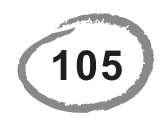
\includegraphics{\rootFolder/_images/test.png}
%}}

%\AddToShipoutPicture*{\BackgroundPic}
%\AddToShipoutPicture*{\NumberPic}

\beginsong{Alegria}[
mlby={António Cláudio},
%sr={Revelation 5:13},
%cr={Public domain.},
%arr={my},
psalterionumber=106,
index={Alegria}]

\beginverse*
Intro: G, G$^{7}$, C, Cm, G, D, G, D (G)
\endverse


\beginverse
\[G]A alegria \[G$^{7}$]está no coração de \[C]quem já conhece \[G]Jesus,
A verdadeira \[Em]paz só tem aquele que \[A]já conhece \[D]Jesus.
O sen\[G]timento mais pre\[G$^{7}$]cioso que \[C]vem do nosso \[Cm]Senhor,
É o \[G]amor, que só \[D]tem quem já conhece \[G]a Jesus.\[C-D]   (repete tudo)
\endverse

\beginchorus
Aleluia, Aleluia, Aleluia, Aleluia. (canon com a estrofe) \\
\endchorus

\beginverse
\chordsoff
O sentimento mais precioso que vem do nosso Senhor, \\
É o amor, \\
Que só tem quem já conhece Jesus. (3x)\\
\endverse

%\begin{wrapfigure}{R}{0.3\textwidth}
%\includegraphics[width=0.3\textwidth]%{\rootFolder/_images/106_Alegria.jpg}
%\end{wrapfigure}	 


%%%%%%%%%%%%%%%%%%%%%%%%%%%%%%%%%%%%%%%%%%%%%%%%%%%%%%%%%%%%%%%%%%%%%%%%%%%
% print guitar tabs used in this song
%%%%%%%%%%%%%%%%%%%%%%%%%%%%%%%%%%%%%%%%%%%%%%%%%%%%%%%%%%%%%%%%%%%%%%%%%%%
\ifbool{gchords}{					% if the guitar chords are to be printed
\vspace{\gchordsVspace}				% set a vertical space of 10 pt 

\gtabD
\gtabA

}									% end if


%\includegraphics[]{106/106_music.pdf} 
%\begin{figure}[] 
%\begin{minipage}[c][\textheight]{\textwidth}
%\includegraphics[]{\rootFolder/score/106_music.pdf} 
%\end{minipage}
%\end{figure}

%%%%%%%%%%%%%%%%%%%%%%%%%%%%%%%%%%%%%%%%%%%%%%%%%%%%%%%%%%%%%%%%%%%%%%%%%%%
% end song latex formating
%%%%%%%%%%%%%%%%%%%%%%%%%%%%%%%%%%%%%%%%%%%%%%%%%%%%%%%%%%%%%%%%%%%%%%%%%%%
\endsong	                   		% end song

	%%%%%%%%%%%%%%%%%%%%%%%%%%%%%%%%%%%%%%%%%%%%%%%%%%%%%%%%%%%%%%%%%%%%%%%%%%%
% this has all the necessary packages and formatting for the document
%%%%%%%%%%%%%%%%%%%%%%%%%%%%%%%%%%%%%%%%%%%%%%%%%%%%%%%%%%%%%%%%%%%%%%%%%%%
%\def \includeFolder{../_include}

% this has all the necessary packages and formatting for the document
\documentclass[10pt,a5paper]{article}

%define include folder
\def \includeFolder{_include}

%packages
\usepackage[left=1cm,right=1cm,top=1cm,bottom=1cm]{geometry}

\usepackage[chorded]{\includeFolder/psalterio} %must check the licence to change the name of the sty file!!!
%\usepackage[chorded]{resources/songs-old} %must check the licence to change the name of the sty file!!!

\usepackage[utf8]{inputenc}

\usepackage{graphicx}
\usepackage{wrapfig}
\usepackage{wallpaper}
\usepackage{color}
\usepackage{eso-pic} %for background pictures
\usepackage[bookmarks]{hyperref} 
%\usepackage{ifthen} %etoolbox is more up to date
\usepackage{etoolbox}


%\usepackage[xetex]{graphicx}
%\usepackage{fontspec,xunicode}
%\defaultfontfeatures{Mapping=tex-text,Scale=MatchLowercase}
%\setmainfont[Scale=.95]{Times}
%\setmonofont{Lucida Sans Typewriter}

%\usepackage[portuguese]{babel}
%\usepackage[latin1]{inputenc}
%\usepackage[utf8]{inputenc}
%\usepackage[T1]{fontenc}
%\usepackage[scaled]{uarial}
%\usepackage{helvet}
%\renewcommand{\familydefault}{\sfdefault}

%this removes the page number
\thispagestyle{empty}
\pagestyle{empty}
\songcolumns{1}

\parindent 0pt

%add background picture
\newcommand\BackgroundPic{
\put(0,0){
\parbox[b][\paperheight]{\paperwidth}{%
\vfill
\centering

\includegraphics[width=\paperwidth,height=\paperheight,
keepaspectratio]{logo.png}%
\vfill
}}}

\newcommand\BottomPic{
\put(0,0){
\includegraphics{_images/bkground_page_bottom.png}
}}





% this includes all the guitar tabs that may be needed
% must complete all the chords used in psalterio

% Cb chords

% C chords
\def \gtabCb{\gtab{Cb}{X32010:X32010}}
\def \gtabC{\gtab{C}{X32010:032010}}
\def \gtabCm{\gtab{Cm}{3:113321:004320}}

\def \gtabCsharpSusFour{\gtab{C\#sus4}{4:XX3341:XX2341}}

% Db chords

% D chords
\def \gtabD{\gtab{D}{X00232:000132}}
\def \gtabDm{\gtab{Dm}{X00231:000231}}
\def \gtabDfour{\gtab{D4}{X00233:000134}}
\def \gtabDseven{\gtab{D7}{X00212:000213}}
\def \gtabDsevenPlus{\gtab{D7+}{X00222:000111}}

% D#/Eb chords
\def \gtabDsharp{\gtab{D\#}{2:XX0232:000132}}

% E chords
\def \gtabE{\gtab{E}{022100:023100}}
\def \gtabEseven{\gtab{E}{020100:020100}}

\def \gtabEm{\gtab{Em}{022000:012000}}
\def \gtabEmSeven{\gtab{Em7}{022030:012040}}

% Gb chords

% F chords
\def \gtabF{\gtab{F}{1:133211:034200}}
\def \gtabFm{\gtab{Fm}{1:133111:034000}}


% F# chords
\def \gtabFsharpMinor{\gtab{F\#m}{2:133111:034000}}
\def \gtabFsharpMinorSeven{\gtab{F\#m7}{2:131131:030040}}

% Gb chords

% G chords
\def \gtabG{\gtab{G}{320033:210034}}
\def \gtabGseven{\gtab{G7}{320001:320001}}
\def \gtabGfret{\gtab{(G)}{3:133211:034200}}
\def \gtabGm{\gtab{Gm}{3:133111:034000}}


% G# / Ab chords

% A chords
\def \gtabA{\gtab{A}{X02220:001230}}
\def \gtabAm{\gtab{Am}{X02210:002310}}
\def \gtabAmSeven{\gtab{Am7}{X02010:002010}}
\def \gtabAfour{\gtab{A4}{X02230:001230}}
\def \gtabAseven{\gtab{A7}{X02020:001030}}

% Bb chords
\def \gtabBb{\gtab{Bb}{X13331}}

% B chords
\def \gtabB{\gtab{B}{X13331:003210}}
\def \gtabBm{\gtab{Bm}{X13321:003420}}
\def \gtabBmSeven{\gtab{Bm7}{X13121:003020}}



% after any { or } at the end of a line inside the macro definition add %, otherwise you'll get an extra space
\newcommand{\guitarTab}[1]{%
\ifstrequal{#1}{Cb}      {\gtab{Cb}{X32010:X32010}      }{}%
\ifstrequal{#1}{C}        { \gtab{C}{X32010:032010}       }{}%
%
%G
%
\ifstrequal{#1}{G}       { \gtab{G}{320033:210034}       }{}%
\ifstrequal{#1}{G7}     { \gtab{G7}{320001:320001}     }{}%
\ifstrequal{#1}{Gfret}  { \gtab{G}{3:133211:034200}    }{}%
\ifstrequal{#1}{Gm}    { \gtab{Gm}{3:133111:034000}  }{}%
} %end \newcommand{\gtab}

%muda aqui o numero da musica em que estas a trabalhar
%\def \selectSong{114}

\providebool{gchords}
\setbool{gchords}{true}

% set guitar chords vertical space separation with lyrics
\def \gchordsVspace{5 mm}

\begin{document}
	
	
	\AddToShipoutPicture*{\BottomPic}
	
	\begin{songs}{}
	
	%format file
	%
%Font Sizes
%
%\tiny
%\scriptsize
%\footnotesize
%\small
%\normalsize
%\large
%\Large
%\LARGE
%\huge
%\Huge


%\renewcommand{\thesongnum}{A\arabic{songnum}}
\renewcommand{\printsongnum}[1]{\sffamily\bfseries\huge\MakeUppercase#1}
\setlength{\songnumwidth}{2cm} % box width
%\renewcommand{\snumbgcolor}{white}

%change font for Title
\renewcommand{\stitlefont}{\sffamily\bfseries\huge\MakeUppercase} %song title

%remove verse numbers
%\noversenumbers 
% make left separation
\setlength{\versenumwidth}{2.0cm}

%verse separations
%\versesep=15pt
%\afterpreludeskip=2pt
%\beforepostludeskip=2pt
%\baselineadj=10pt

% separation between chords and lyrics
\renewcommand{\clineparams}{ 
\baselineskip=10pt 
%\lineskiplimit=2pt 
%\lineskip=5pt
}

% change font for lyrics
%\renewcommand{\lyricfont}{\sffamily}
%\renewcommand{\lyricfont}{\sffamily\small}
\renewcommand{\lyricfont}{\sffamily\large}
%\renewcommand{\chorusfont}{\sffamily}
\renewcommand{\chorusfont}{\sffamily\large}

%change the Chords formatting
\renewcommand{\printchord}[1]{\sffamily\color{red}\it\normalsize#1}

%check http://www.tug.org/pracjourn/2006-1/schmidt/schmidt.pdf


%\renewcommand{\songauthors}[1]{tete #1}


%\renewcommand{\extendpostlude}
%{ \songcopyright\ \songlicense\unskip \ Used with permission.}

\setlength{\cbarwidth}{0pt}
\setlength{\sbarheight}{0pt}

% music anf lyrics by
\newcommand{\musicLyricsBy}{} 
\newsongkey{mlby}{\def\musicLyricsBy{}}
                 {\def\musicLyricsBy{\sffamily\it\small letra e música por #1\par}}

% music anf lyrics by
\newcommand{\musicby}{} 
\newsongkey{music}{\def\musicby{}}
                 {\def\musicby{\sffamily\it\small música: #1\par}}

% music anf lyrics by
\newcommand{\lyricsby}{} 
\newsongkey{lyrics}{\def\lyricsby{}}
                 {\def\lyricsby{\sffamily\it\small letra: #1\par}}

%\renewcommand{\sharpsymbol}{\ensuremath{^\sharp}}
\renewcommand{\extendprelude}{
  \showrefs\showauthors 
  %{\bfseries\musicLyricsBy}
  {\bfseries\musicby}
  {\bfseries\lyricsby}
}

\def \gtabsOn{1}
	

%%%%%%%%%%%%%%%%%%%%%%%%%%%%%%%%%%%%%%%%%%%%%%%%%%%%%%%%%%%%%%%%%%%%%%%%%%%
% set song number
%%%%%%%%%%%%%%%%%%%%%%%%%%%%%%%%%%%%%%%%%%%%%%%%%%%%%%%%%%%%%%%%%%%%%%%%%%%
\setcounter{songnum}{141}

%%%%%%%%%%%%%%%%%%%%%%%%%%%%%%%%%%%%%%%%%%%%%%%%%%%%%%%%%%%%%%%%%%%%%%%%%%%
% begin song latex formating, set the title and other info
%%%%%%%%%%%%%%%%%%%%%%%%%%%%%%%%%%%%%%%%%%%%%%%%%%%%%%%%%%%%%%%%%%%%%%%%%%%
% song title
\beginsong{Brilhando Cada Vez Mais}[
% music and lyric by
% mlby={},
% lyrics
%lyrics={}, 
% music by
%music={},
% bible verse
%sr={},
% licence/copyright
%cr={Public domain.},
% arrangement by
%arr={},
psalterionumber=141,
% index title
index={Brilhando Cada Vez Mais}]

%%%%%%%%%%%%%%%%%%%%%%%%%%%%%%%%%%%%%%%%%%%%%%%%%%%%%%%%%%%%%%%%%%%%%%%%%%%
% section #1: verse 
%%%%%%%%%%%%%%%%%%%%%%%%%%%%%%%%%%%%%%%%%%%%%%%%%%%%%%%%%%%%%%%%%%%%%%%%%%%
\beginverse
\[D]O Tição pensa \[A]primeiro em Jesus
\[G]E nos \[A]outros
\[D]O Tição lê a \[A]Bíblia e \[G]ora cada \[A]dia
\[Bm]O Tição é \[F#m]honesto e verdadeiro
\[G]Obediente e \[A]amável
\[A]E o nosso voto é:
\endverse

%%%%%%%%%%%%%%%%%%%%%%%%%%%%%%%%%%%%%%%%%%%%%%%%%%%%%%%%%%%%%%%%%%%%%%%%%%%
% section #2: chorus 
%%%%%%%%%%%%%%%%%%%%%%%%%%%%%%%%%%%%%%%%%%%%%%%%%%%%%%%%%%%%%%%%%%%%%%%%%%%
\beginchorus
Com Jesus e a \[A]ajuda de todos do \[G]clube
Prometo \[A]fazer sempre o meu melhor
\[D]Brilhando \[A]cada vez mais,
\[G]Cada vez \[A4-A]mais
\[D]Brilhando \[A]cada vez mais,
\[G]Cada vez \[A4-A-D]mais
\endchorus


%%%%%%%%%%%%%%%%%%%%%%%%%%%%%%%%%%%%%%%%%%%%%%%%%%%%%%%%%%%%%%%%%%%%%%%%%%%
% print guitar tabs used in this song
%%%%%%%%%%%%%%%%%%%%%%%%%%%%%%%%%%%%%%%%%%%%%%%%%%%%%%%%%%%%%%%%%%%%%%%%%%%
% if the guitar chords are to be printed
\ifbool{gchords}{
% set a vertical space of 10 pt 
\vspace{\gchordsVspace}
} % end if

%%%%%%%%%%%%%%%%%%%%%%%%%%%%%%%%%%%%%%%%%%%%%%%%%%%%%%%%%%%%%%%%%%%%%%%%%%%
% end song latex formating
%%%%%%%%%%%%%%%%%%%%%%%%%%%%%%%%%%%%%%%%%%%%%%%%%%%%%%%%%%%%%%%%%%%%%%%%%%%
% end song
\endsong

%include song latex footer
%	 %lilypond-book --output=out --pdf  106single.tex
	 %\lilypondfile[]{E_101.ly}
	
\end{document}
	%%%%%%%%%%%%%%%%%%%%%%%%%%%%%%%%%%%%%%%%%%%%%%%%%%%%%%%%%%%%%%%%%%%%%%%%%%%
% this has all the necessary packages and formatting for the document
%%%%%%%%%%%%%%%%%%%%%%%%%%%%%%%%%%%%%%%%%%%%%%%%%%%%%%%%%%%%%%%%%%%%%%%%%%%
%\def \includeFolder{../_include}

% this has all the necessary packages and formatting for the document
\documentclass[10pt,a5paper]{article}

%define include folder
\def \includeFolder{_include}

%packages
\usepackage[left=1cm,right=1cm,top=1cm,bottom=1cm]{geometry}

\usepackage[chorded]{\includeFolder/psalterio} %must check the licence to change the name of the sty file!!!
%\usepackage[chorded]{resources/songs-old} %must check the licence to change the name of the sty file!!!

\usepackage[utf8]{inputenc}

\usepackage{graphicx}
\usepackage{wrapfig}
\usepackage{wallpaper}
\usepackage{color}
\usepackage{eso-pic} %for background pictures
\usepackage[bookmarks]{hyperref} 
%\usepackage{ifthen} %etoolbox is more up to date
\usepackage{etoolbox}


%\usepackage[xetex]{graphicx}
%\usepackage{fontspec,xunicode}
%\defaultfontfeatures{Mapping=tex-text,Scale=MatchLowercase}
%\setmainfont[Scale=.95]{Times}
%\setmonofont{Lucida Sans Typewriter}

%\usepackage[portuguese]{babel}
%\usepackage[latin1]{inputenc}
%\usepackage[utf8]{inputenc}
%\usepackage[T1]{fontenc}
%\usepackage[scaled]{uarial}
%\usepackage{helvet}
%\renewcommand{\familydefault}{\sfdefault}

%this removes the page number
\thispagestyle{empty}
\pagestyle{empty}
\songcolumns{1}

\parindent 0pt

%add background picture
\newcommand\BackgroundPic{
\put(0,0){
\parbox[b][\paperheight]{\paperwidth}{%
\vfill
\centering

\includegraphics[width=\paperwidth,height=\paperheight,
keepaspectratio]{logo.png}%
\vfill
}}}

\newcommand\BottomPic{
\put(0,0){
\includegraphics{_images/bkground_page_bottom.png}
}}





% this includes all the guitar tabs that may be needed
% must complete all the chords used in psalterio

% Cb chords

% C chords
\def \gtabCb{\gtab{Cb}{X32010:X32010}}
\def \gtabC{\gtab{C}{X32010:032010}}
\def \gtabCm{\gtab{Cm}{3:113321:004320}}

\def \gtabCsharpSusFour{\gtab{C\#sus4}{4:XX3341:XX2341}}

% Db chords

% D chords
\def \gtabD{\gtab{D}{X00232:000132}}
\def \gtabDm{\gtab{Dm}{X00231:000231}}
\def \gtabDfour{\gtab{D4}{X00233:000134}}
\def \gtabDseven{\gtab{D7}{X00212:000213}}
\def \gtabDsevenPlus{\gtab{D7+}{X00222:000111}}

% D#/Eb chords
\def \gtabDsharp{\gtab{D\#}{2:XX0232:000132}}

% E chords
\def \gtabE{\gtab{E}{022100:023100}}
\def \gtabEseven{\gtab{E}{020100:020100}}

\def \gtabEm{\gtab{Em}{022000:012000}}
\def \gtabEmSeven{\gtab{Em7}{022030:012040}}

% Gb chords

% F chords
\def \gtabF{\gtab{F}{1:133211:034200}}
\def \gtabFm{\gtab{Fm}{1:133111:034000}}


% F# chords
\def \gtabFsharpMinor{\gtab{F\#m}{2:133111:034000}}
\def \gtabFsharpMinorSeven{\gtab{F\#m7}{2:131131:030040}}

% Gb chords

% G chords
\def \gtabG{\gtab{G}{320033:210034}}
\def \gtabGseven{\gtab{G7}{320001:320001}}
\def \gtabGfret{\gtab{(G)}{3:133211:034200}}
\def \gtabGm{\gtab{Gm}{3:133111:034000}}


% G# / Ab chords

% A chords
\def \gtabA{\gtab{A}{X02220:001230}}
\def \gtabAm{\gtab{Am}{X02210:002310}}
\def \gtabAmSeven{\gtab{Am7}{X02010:002010}}
\def \gtabAfour{\gtab{A4}{X02230:001230}}
\def \gtabAseven{\gtab{A7}{X02020:001030}}

% Bb chords
\def \gtabBb{\gtab{Bb}{X13331}}

% B chords
\def \gtabB{\gtab{B}{X13331:003210}}
\def \gtabBm{\gtab{Bm}{X13321:003420}}
\def \gtabBmSeven{\gtab{Bm7}{X13121:003020}}



% after any { or } at the end of a line inside the macro definition add %, otherwise you'll get an extra space
\newcommand{\guitarTab}[1]{%
\ifstrequal{#1}{Cb}      {\gtab{Cb}{X32010:X32010}      }{}%
\ifstrequal{#1}{C}        { \gtab{C}{X32010:032010}       }{}%
%
%G
%
\ifstrequal{#1}{G}       { \gtab{G}{320033:210034}       }{}%
\ifstrequal{#1}{G7}     { \gtab{G7}{320001:320001}     }{}%
\ifstrequal{#1}{Gfret}  { \gtab{G}{3:133211:034200}    }{}%
\ifstrequal{#1}{Gm}    { \gtab{Gm}{3:133111:034000}  }{}%
} %end \newcommand{\gtab}

%muda aqui o numero da musica em que estas a trabalhar
%\def \selectSong{114}

\providebool{gchords}
\setbool{gchords}{true}

% set guitar chords vertical space separation with lyrics
\def \gchordsVspace{5 mm}

\begin{document}
	
	
	\AddToShipoutPicture*{\BottomPic}
	
	\begin{songs}{}
	
	%format file
	%
%Font Sizes
%
%\tiny
%\scriptsize
%\footnotesize
%\small
%\normalsize
%\large
%\Large
%\LARGE
%\huge
%\Huge


%\renewcommand{\thesongnum}{A\arabic{songnum}}
\renewcommand{\printsongnum}[1]{\sffamily\bfseries\huge\MakeUppercase#1}
\setlength{\songnumwidth}{2cm} % box width
%\renewcommand{\snumbgcolor}{white}

%change font for Title
\renewcommand{\stitlefont}{\sffamily\bfseries\huge\MakeUppercase} %song title

%remove verse numbers
%\noversenumbers 
% make left separation
\setlength{\versenumwidth}{2.0cm}

%verse separations
%\versesep=15pt
%\afterpreludeskip=2pt
%\beforepostludeskip=2pt
%\baselineadj=10pt

% separation between chords and lyrics
\renewcommand{\clineparams}{ 
\baselineskip=10pt 
%\lineskiplimit=2pt 
%\lineskip=5pt
}

% change font for lyrics
%\renewcommand{\lyricfont}{\sffamily}
%\renewcommand{\lyricfont}{\sffamily\small}
\renewcommand{\lyricfont}{\sffamily\large}
%\renewcommand{\chorusfont}{\sffamily}
\renewcommand{\chorusfont}{\sffamily\large}

%change the Chords formatting
\renewcommand{\printchord}[1]{\sffamily\color{red}\it\normalsize#1}

%check http://www.tug.org/pracjourn/2006-1/schmidt/schmidt.pdf


%\renewcommand{\songauthors}[1]{tete #1}


%\renewcommand{\extendpostlude}
%{ \songcopyright\ \songlicense\unskip \ Used with permission.}

\setlength{\cbarwidth}{0pt}
\setlength{\sbarheight}{0pt}

% music anf lyrics by
\newcommand{\musicLyricsBy}{} 
\newsongkey{mlby}{\def\musicLyricsBy{}}
                 {\def\musicLyricsBy{\sffamily\it\small letra e música por #1\par}}

% music anf lyrics by
\newcommand{\musicby}{} 
\newsongkey{music}{\def\musicby{}}
                 {\def\musicby{\sffamily\it\small música: #1\par}}

% music anf lyrics by
\newcommand{\lyricsby}{} 
\newsongkey{lyrics}{\def\lyricsby{}}
                 {\def\lyricsby{\sffamily\it\small letra: #1\par}}

%\renewcommand{\sharpsymbol}{\ensuremath{^\sharp}}
\renewcommand{\extendprelude}{
  \showrefs\showauthors 
  %{\bfseries\musicLyricsBy}
  {\bfseries\musicby}
  {\bfseries\lyricsby}
}

\def \gtabsOn{1}
	

%%%%%%%%%%%%%%%%%%%%%%%%%%%%%%%%%%%%%%%%%%%%%%%%%%%%%%%%%%%%%%%%%%%%%%%%%%%
% set song number
%%%%%%%%%%%%%%%%%%%%%%%%%%%%%%%%%%%%%%%%%%%%%%%%%%%%%%%%%%%%%%%%%%%%%%%%%%%
\setcounter{songnum}{101}													% song number

%%%%%%%%%%%%%%%%%%%%%%%%%%%%%%%%%%%%%%%%%%%%%%%%%%%%%%%%%%%%%%%%%%%%%%%%%%%
% begin song latex formating, set the title and other info
%%%%%%%%%%%%%%%%%%%%%%%%%%%%%%%%%%%%%%%%%%%%%%%%%%%%%%%%%%%%%%%%%%%%%%%%%%%
\beginsong{A Bandeira do Céu}[	                               						% song title ...
	%mlby={},                                            							% music and lyric by ...	
	%sr={Revelation 5:13},                               						% bible verse  ...	
	%cr={Public domain.},                               						% licence  ...	
	%arr={my},                                          							% arrangement by  ...	
	index={A Bandeira do Céu}]                                   						% index title ...	
            
%%%%%%%%%%%%%%%%%%%%%%%%%%%%%%%%%%%%%%%%%%%%%%%%%%%%%%%%%%%%%%%%%%%%%%%%%%%            
% verse #1
%%%%%%%%%%%%%%%%%%%%%%%%%%%%%%%%%%%%%%%%%%%%%%%%%%%%%%%%%%%%%%%%%%%%%%%%%%%
\beginverse                                           								% start verse
\[G]Nós pode\[D]mos anun\[C]ciar ao mundo in\[D]teiro
\[G]Que há vi\[D]da ao la\[C]do de Je\[D]sus
\[G]Nós pode\[D]mos procla\[C]mar o evange\[D]lho da \[D]cruz
\[Em](Je\[C]sus, \[Em]Je\[C]sus)\[D] (repete)
\endverse	                                           								% end verse

%%%%%%%%%%%%%%%%%%%%%%%%%%%%%%%%%%%%%%%%%%%%%%%%%%%%%%%%%%%%%%%%%%%%%%%%%%%
% chorus
%%%%%%%%%%%%%%%%%%%%%%%%%%%%%%%%%%%%%%%%%%%%%%%%%%%%%%%%%%%%%%%%%%%%%%%%%%%
\beginchorus                                          							% start chorus
\[G]Nós pode\[D]mos haste\[Em]ar
A bandei\[G]ra \[D]do \[G]céu
Vamos \[D]todos agit\[Em]ar
A ban\[C]deira \[D]do \[G]céu
Entre to\[D]dos nós po\[Em]demos conse\[C]guir
Levant\[Am]ar no mundo in\[C]teiro
A bandei\[C]ra \[D]do \[G]céu
\[Em]Je\[C]sus
\[Em]Je\[Am]sus

\chordsoff                                           								% chords formating off
A bandeira do céu
Nós podemos hastear Vamos todos agitar
A bandeira do céu
\chordson   																			% chords formating on
\endchorus	                                          								% end chorus

%%%%%%%%%%%%%%%%%%%%%%%%%%%%%%%%%%%%%%%%%%%%%%%%%%%%%%%%%%%%%%%%%%%%%%%%%%%
% print guitar tabs used in this song
%%%%%%%%%%%%%%%%%%%%%%%%%%%%%%%%%%%%%%%%%%%%%%%%%%%%%%%%%%%%%%%%%%%%%%%%%%%
\ifbool{gchords}{																	% if the guitar chords are to be printed
\vspace{\gchordsVspace}													% set a vertical space of 10 pt 

\gtabC
\gtabD
\gtabG
\gtabEm
\gtabAm

}																							% end if

%%%%%%%%%%%%%%%%%%%%%%%%%%%%%%%%%%%%%%%%%%%%%%%%%%%%%%%%%%%%%%%%%%%%%%%%%%%
% end song latex formating
%%%%%%%%%%%%%%%%%%%%%%%%%%%%%%%%%%%%%%%%%%%%%%%%%%%%%%%%%%%%%%%%%%%%%%%%%%%
\endsong	                                            								% end song
%	 %lilypond-book --output=out --pdf  106single.tex
	 %\lilypondfile[]{E_101.ly}
	
\end{document}
	%%%%%%%%%%%%%%%%%%%%%%%%%%%%%%%%%%%%%%%%%%%%%%%%%%%%%%%%%%%%%%%%%%%%%%%%%%%
% this has all the necessary packages and formatting for the document
%%%%%%%%%%%%%%%%%%%%%%%%%%%%%%%%%%%%%%%%%%%%%%%%%%%%%%%%%%%%%%%%%%%%%%%%%%%
%\def \includeFolder{../_include}

% this has all the necessary packages and formatting for the document
\documentclass[10pt,a5paper]{article}

%define include folder
\def \includeFolder{_include}

%packages
\usepackage[left=1cm,right=1cm,top=1cm,bottom=1cm]{geometry}

\usepackage[chorded]{\includeFolder/psalterio} %must check the licence to change the name of the sty file!!!
%\usepackage[chorded]{resources/songs-old} %must check the licence to change the name of the sty file!!!

\usepackage[utf8]{inputenc}

\usepackage{graphicx}
\usepackage{wrapfig}
\usepackage{wallpaper}
\usepackage{color}
\usepackage{eso-pic} %for background pictures
\usepackage[bookmarks]{hyperref} 
%\usepackage{ifthen} %etoolbox is more up to date
\usepackage{etoolbox}


%\usepackage[xetex]{graphicx}
%\usepackage{fontspec,xunicode}
%\defaultfontfeatures{Mapping=tex-text,Scale=MatchLowercase}
%\setmainfont[Scale=.95]{Times}
%\setmonofont{Lucida Sans Typewriter}

%\usepackage[portuguese]{babel}
%\usepackage[latin1]{inputenc}
%\usepackage[utf8]{inputenc}
%\usepackage[T1]{fontenc}
%\usepackage[scaled]{uarial}
%\usepackage{helvet}
%\renewcommand{\familydefault}{\sfdefault}

%this removes the page number
\thispagestyle{empty}
\pagestyle{empty}
\songcolumns{1}

\parindent 0pt

%add background picture
\newcommand\BackgroundPic{
\put(0,0){
\parbox[b][\paperheight]{\paperwidth}{%
\vfill
\centering

\includegraphics[width=\paperwidth,height=\paperheight,
keepaspectratio]{logo.png}%
\vfill
}}}

\newcommand\BottomPic{
\put(0,0){
\includegraphics{_images/bkground_page_bottom.png}
}}





% this includes all the guitar tabs that may be needed
% must complete all the chords used in psalterio

% Cb chords

% C chords
\def \gtabCb{\gtab{Cb}{X32010:X32010}}
\def \gtabC{\gtab{C}{X32010:032010}}
\def \gtabCm{\gtab{Cm}{3:113321:004320}}

\def \gtabCsharpSusFour{\gtab{C\#sus4}{4:XX3341:XX2341}}

% Db chords

% D chords
\def \gtabD{\gtab{D}{X00232:000132}}
\def \gtabDm{\gtab{Dm}{X00231:000231}}
\def \gtabDfour{\gtab{D4}{X00233:000134}}
\def \gtabDseven{\gtab{D7}{X00212:000213}}
\def \gtabDsevenPlus{\gtab{D7+}{X00222:000111}}

% D#/Eb chords
\def \gtabDsharp{\gtab{D\#}{2:XX0232:000132}}

% E chords
\def \gtabE{\gtab{E}{022100:023100}}
\def \gtabEseven{\gtab{E}{020100:020100}}

\def \gtabEm{\gtab{Em}{022000:012000}}
\def \gtabEmSeven{\gtab{Em7}{022030:012040}}

% Gb chords

% F chords
\def \gtabF{\gtab{F}{1:133211:034200}}
\def \gtabFm{\gtab{Fm}{1:133111:034000}}


% F# chords
\def \gtabFsharpMinor{\gtab{F\#m}{2:133111:034000}}
\def \gtabFsharpMinorSeven{\gtab{F\#m7}{2:131131:030040}}

% Gb chords

% G chords
\def \gtabG{\gtab{G}{320033:210034}}
\def \gtabGseven{\gtab{G7}{320001:320001}}
\def \gtabGfret{\gtab{(G)}{3:133211:034200}}
\def \gtabGm{\gtab{Gm}{3:133111:034000}}


% G# / Ab chords

% A chords
\def \gtabA{\gtab{A}{X02220:001230}}
\def \gtabAm{\gtab{Am}{X02210:002310}}
\def \gtabAmSeven{\gtab{Am7}{X02010:002010}}
\def \gtabAfour{\gtab{A4}{X02230:001230}}
\def \gtabAseven{\gtab{A7}{X02020:001030}}

% Bb chords
\def \gtabBb{\gtab{Bb}{X13331}}

% B chords
\def \gtabB{\gtab{B}{X13331:003210}}
\def \gtabBm{\gtab{Bm}{X13321:003420}}
\def \gtabBmSeven{\gtab{Bm7}{X13121:003020}}



% after any { or } at the end of a line inside the macro definition add %, otherwise you'll get an extra space
\newcommand{\guitarTab}[1]{%
\ifstrequal{#1}{Cb}      {\gtab{Cb}{X32010:X32010}      }{}%
\ifstrequal{#1}{C}        { \gtab{C}{X32010:032010}       }{}%
%
%G
%
\ifstrequal{#1}{G}       { \gtab{G}{320033:210034}       }{}%
\ifstrequal{#1}{G7}     { \gtab{G7}{320001:320001}     }{}%
\ifstrequal{#1}{Gfret}  { \gtab{G}{3:133211:034200}    }{}%
\ifstrequal{#1}{Gm}    { \gtab{Gm}{3:133111:034000}  }{}%
} %end \newcommand{\gtab}

%muda aqui o numero da musica em que estas a trabalhar
%\def \selectSong{114}

\providebool{gchords}
\setbool{gchords}{true}

% set guitar chords vertical space separation with lyrics
\def \gchordsVspace{5 mm}

\begin{document}
	
	
	\AddToShipoutPicture*{\BottomPic}
	
	\begin{songs}{}
	
	%format file
	%
%Font Sizes
%
%\tiny
%\scriptsize
%\footnotesize
%\small
%\normalsize
%\large
%\Large
%\LARGE
%\huge
%\Huge


%\renewcommand{\thesongnum}{A\arabic{songnum}}
\renewcommand{\printsongnum}[1]{\sffamily\bfseries\huge\MakeUppercase#1}
\setlength{\songnumwidth}{2cm} % box width
%\renewcommand{\snumbgcolor}{white}

%change font for Title
\renewcommand{\stitlefont}{\sffamily\bfseries\huge\MakeUppercase} %song title

%remove verse numbers
%\noversenumbers 
% make left separation
\setlength{\versenumwidth}{2.0cm}

%verse separations
%\versesep=15pt
%\afterpreludeskip=2pt
%\beforepostludeskip=2pt
%\baselineadj=10pt

% separation between chords and lyrics
\renewcommand{\clineparams}{ 
\baselineskip=10pt 
%\lineskiplimit=2pt 
%\lineskip=5pt
}

% change font for lyrics
%\renewcommand{\lyricfont}{\sffamily}
%\renewcommand{\lyricfont}{\sffamily\small}
\renewcommand{\lyricfont}{\sffamily\large}
%\renewcommand{\chorusfont}{\sffamily}
\renewcommand{\chorusfont}{\sffamily\large}

%change the Chords formatting
\renewcommand{\printchord}[1]{\sffamily\color{red}\it\normalsize#1}

%check http://www.tug.org/pracjourn/2006-1/schmidt/schmidt.pdf


%\renewcommand{\songauthors}[1]{tete #1}


%\renewcommand{\extendpostlude}
%{ \songcopyright\ \songlicense\unskip \ Used with permission.}

\setlength{\cbarwidth}{0pt}
\setlength{\sbarheight}{0pt}

% music anf lyrics by
\newcommand{\musicLyricsBy}{} 
\newsongkey{mlby}{\def\musicLyricsBy{}}
                 {\def\musicLyricsBy{\sffamily\it\small letra e música por #1\par}}

% music anf lyrics by
\newcommand{\musicby}{} 
\newsongkey{music}{\def\musicby{}}
                 {\def\musicby{\sffamily\it\small música: #1\par}}

% music anf lyrics by
\newcommand{\lyricsby}{} 
\newsongkey{lyrics}{\def\lyricsby{}}
                 {\def\lyricsby{\sffamily\it\small letra: #1\par}}

%\renewcommand{\sharpsymbol}{\ensuremath{^\sharp}}
\renewcommand{\extendprelude}{
  \showrefs\showauthors 
  %{\bfseries\musicLyricsBy}
  {\bfseries\musicby}
  {\bfseries\lyricsby}
}

\def \gtabsOn{1}
	

%\setcounter{songnum}{101}

%%%%%%%%%%%%%%%%%%%%%%%%%%%%%%%%%%%%%%%%%%%%%%%%%%%%%%%%%%%%%%%%%%%%%%%%%%%
% begin song latex formating, set the title and other info
%%%%%%%%%%%%%%%%%%%%%%%%%%%%%%%%%%%%%%%%%%%%%%%%%%%%%%%%%%%%%%%%%%%%%%%%%%%
\beginsong{Digno de Glória}[
mlby={Asaph Borba},
%sr={Revelation 5:13},              % bible verse  ...	
%cr={Public domain.},               % licence  ...	
%arr={my},                                % arrangement by  ...	
index={Digno de Glória}]
            
%%%%%%%%%%%%%%%%%%%%%%%%%%%%%%%%%%%%%%%%%%%%%%%%%%%%%%%%%%%%%%%%%%%%%%%%%%%            
% verse #1
%%%%%%%%%%%%%%%%%%%%%%%%%%%%%%%%%%%%%%%%%%%%%%%%%%%%%%%%%%%%%%%%%%%%%%%%%%%
\beginverse                                           								% start verse
Digno de \[C]gló\[Em]ria e \[Am]honra,
Levan\[F]tamos nossas \[Dm]mãos pra Teu \[G]nome exal\[G7]tar.
Digno de \[C]gló\[Em]ria e \[Am]honra,
Levan\[F]tamos nossas \[Dm]mãos pra Teu \[G]nome exal\[G7]tar.
\endverse	                                           								% end verse

%%%%%%%%%%%%%%%%%%%%%%%%%%%%%%%%%%%%%%%%%%%%%%%%%%%%%%%%%%%%%%%%%%%%%%%%%%%
% chorus
%%%%%%%%%%%%%%%%%%%%%%%%%%%%%%%%%%%%%%%%%%%%%%%%%%%%%%%%%%%%%%%%%%%%%%%%%%%
\beginchorus                                          							% start chorus
Porque grande És \[C]Tu, mara\[Em]vilhas fazes \[Am]Tu,
Não há \[Em]outro igual a\[F Em Dm] Ti,
Não há \[G]outro igual a \[G7]Ti,
\endchorus	                                          								% end chorus


%%%%%%%%%%%%%%%%%%%%%%%%%%%%%%%%%%%%%%%%%%%%%%%%%%%%%%%%%%%%%%%%%%%%%%%%%%%
% print guitar tabs used in this song
%%%%%%%%%%%%%%%%%%%%%%%%%%%%%%%%%%%%%%%%%%%%%%%%%%%%%%%%%%%%%%%%%%%%%%%%%%%
\ifbool{gchords}{																	% if the guitar chords are to be printed
\vspace{\gchordsVspace}													% set a vertical space of 10 pt 
}																							% end if

%%%%%%%%%%%%%%%%%%%%%%%%%%%%%%%%%%%%%%%%%%%%%%%%%%%%%%%%%%%%%%%%%%%%%%%%%%%
% end song latex formating
%%%%%%%%%%%%%%%%%%%%%%%%%%%%%%%%%%%%%%%%%%%%%%%%%%%%%%%%%%%%%%%%%%%%%%%%%%%
\endsong	                                            								% end song
%	 %lilypond-book --output=out --pdf  106single.tex
	 %\lilypondfile[]{E_101.ly}
	
\end{document}
	%%%%%%%%%%%%%%%%%%%%%%%%%%%%%%%%%%%%%%%%%%%%%%%%%%%%%%%%%%%%%%%%%%%%%%%%%%%
% this has all the necessary packages and formatting for the document
%%%%%%%%%%%%%%%%%%%%%%%%%%%%%%%%%%%%%%%%%%%%%%%%%%%%%%%%%%%%%%%%%%%%%%%%%%%
%\def \includeFolder{../_include}

% this has all the necessary packages and formatting for the document
\documentclass[10pt,a5paper]{article}

%define include folder
\def \includeFolder{_include}

%packages
\usepackage[left=1cm,right=1cm,top=1cm,bottom=1cm]{geometry}

\usepackage[chorded]{\includeFolder/psalterio} %must check the licence to change the name of the sty file!!!
%\usepackage[chorded]{resources/songs-old} %must check the licence to change the name of the sty file!!!

\usepackage[utf8]{inputenc}

\usepackage{graphicx}
\usepackage{wrapfig}
\usepackage{wallpaper}
\usepackage{color}
\usepackage{eso-pic} %for background pictures
\usepackage[bookmarks]{hyperref} 
%\usepackage{ifthen} %etoolbox is more up to date
\usepackage{etoolbox}


%\usepackage[xetex]{graphicx}
%\usepackage{fontspec,xunicode}
%\defaultfontfeatures{Mapping=tex-text,Scale=MatchLowercase}
%\setmainfont[Scale=.95]{Times}
%\setmonofont{Lucida Sans Typewriter}

%\usepackage[portuguese]{babel}
%\usepackage[latin1]{inputenc}
%\usepackage[utf8]{inputenc}
%\usepackage[T1]{fontenc}
%\usepackage[scaled]{uarial}
%\usepackage{helvet}
%\renewcommand{\familydefault}{\sfdefault}

%this removes the page number
\thispagestyle{empty}
\pagestyle{empty}
\songcolumns{1}

\parindent 0pt

%add background picture
\newcommand\BackgroundPic{
\put(0,0){
\parbox[b][\paperheight]{\paperwidth}{%
\vfill
\centering

\includegraphics[width=\paperwidth,height=\paperheight,
keepaspectratio]{logo.png}%
\vfill
}}}

\newcommand\BottomPic{
\put(0,0){
\includegraphics{_images/bkground_page_bottom.png}
}}





% this includes all the guitar tabs that may be needed
% must complete all the chords used in psalterio

% Cb chords

% C chords
\def \gtabCb{\gtab{Cb}{X32010:X32010}}
\def \gtabC{\gtab{C}{X32010:032010}}
\def \gtabCm{\gtab{Cm}{3:113321:004320}}

\def \gtabCsharpSusFour{\gtab{C\#sus4}{4:XX3341:XX2341}}

% Db chords

% D chords
\def \gtabD{\gtab{D}{X00232:000132}}
\def \gtabDm{\gtab{Dm}{X00231:000231}}
\def \gtabDfour{\gtab{D4}{X00233:000134}}
\def \gtabDseven{\gtab{D7}{X00212:000213}}
\def \gtabDsevenPlus{\gtab{D7+}{X00222:000111}}

% D#/Eb chords
\def \gtabDsharp{\gtab{D\#}{2:XX0232:000132}}

% E chords
\def \gtabE{\gtab{E}{022100:023100}}
\def \gtabEseven{\gtab{E}{020100:020100}}

\def \gtabEm{\gtab{Em}{022000:012000}}
\def \gtabEmSeven{\gtab{Em7}{022030:012040}}

% Gb chords

% F chords
\def \gtabF{\gtab{F}{1:133211:034200}}
\def \gtabFm{\gtab{Fm}{1:133111:034000}}


% F# chords
\def \gtabFsharpMinor{\gtab{F\#m}{2:133111:034000}}
\def \gtabFsharpMinorSeven{\gtab{F\#m7}{2:131131:030040}}

% Gb chords

% G chords
\def \gtabG{\gtab{G}{320033:210034}}
\def \gtabGseven{\gtab{G7}{320001:320001}}
\def \gtabGfret{\gtab{(G)}{3:133211:034200}}
\def \gtabGm{\gtab{Gm}{3:133111:034000}}


% G# / Ab chords

% A chords
\def \gtabA{\gtab{A}{X02220:001230}}
\def \gtabAm{\gtab{Am}{X02210:002310}}
\def \gtabAmSeven{\gtab{Am7}{X02010:002010}}
\def \gtabAfour{\gtab{A4}{X02230:001230}}
\def \gtabAseven{\gtab{A7}{X02020:001030}}

% Bb chords
\def \gtabBb{\gtab{Bb}{X13331}}

% B chords
\def \gtabB{\gtab{B}{X13331:003210}}
\def \gtabBm{\gtab{Bm}{X13321:003420}}
\def \gtabBmSeven{\gtab{Bm7}{X13121:003020}}



% after any { or } at the end of a line inside the macro definition add %, otherwise you'll get an extra space
\newcommand{\guitarTab}[1]{%
\ifstrequal{#1}{Cb}      {\gtab{Cb}{X32010:X32010}      }{}%
\ifstrequal{#1}{C}        { \gtab{C}{X32010:032010}       }{}%
%
%G
%
\ifstrequal{#1}{G}       { \gtab{G}{320033:210034}       }{}%
\ifstrequal{#1}{G7}     { \gtab{G7}{320001:320001}     }{}%
\ifstrequal{#1}{Gfret}  { \gtab{G}{3:133211:034200}    }{}%
\ifstrequal{#1}{Gm}    { \gtab{Gm}{3:133111:034000}  }{}%
} %end \newcommand{\gtab}

%muda aqui o numero da musica em que estas a trabalhar
%\def \selectSong{114}

\providebool{gchords}
\setbool{gchords}{true}

% set guitar chords vertical space separation with lyrics
\def \gchordsVspace{5 mm}

\begin{document}
	
	
	\AddToShipoutPicture*{\BottomPic}
	
	\begin{songs}{}
	
	%format file
	%
%Font Sizes
%
%\tiny
%\scriptsize
%\footnotesize
%\small
%\normalsize
%\large
%\Large
%\LARGE
%\huge
%\Huge


%\renewcommand{\thesongnum}{A\arabic{songnum}}
\renewcommand{\printsongnum}[1]{\sffamily\bfseries\huge\MakeUppercase#1}
\setlength{\songnumwidth}{2cm} % box width
%\renewcommand{\snumbgcolor}{white}

%change font for Title
\renewcommand{\stitlefont}{\sffamily\bfseries\huge\MakeUppercase} %song title

%remove verse numbers
%\noversenumbers 
% make left separation
\setlength{\versenumwidth}{2.0cm}

%verse separations
%\versesep=15pt
%\afterpreludeskip=2pt
%\beforepostludeskip=2pt
%\baselineadj=10pt

% separation between chords and lyrics
\renewcommand{\clineparams}{ 
\baselineskip=10pt 
%\lineskiplimit=2pt 
%\lineskip=5pt
}

% change font for lyrics
%\renewcommand{\lyricfont}{\sffamily}
%\renewcommand{\lyricfont}{\sffamily\small}
\renewcommand{\lyricfont}{\sffamily\large}
%\renewcommand{\chorusfont}{\sffamily}
\renewcommand{\chorusfont}{\sffamily\large}

%change the Chords formatting
\renewcommand{\printchord}[1]{\sffamily\color{red}\it\normalsize#1}

%check http://www.tug.org/pracjourn/2006-1/schmidt/schmidt.pdf


%\renewcommand{\songauthors}[1]{tete #1}


%\renewcommand{\extendpostlude}
%{ \songcopyright\ \songlicense\unskip \ Used with permission.}

\setlength{\cbarwidth}{0pt}
\setlength{\sbarheight}{0pt}

% music anf lyrics by
\newcommand{\musicLyricsBy}{} 
\newsongkey{mlby}{\def\musicLyricsBy{}}
                 {\def\musicLyricsBy{\sffamily\it\small letra e música por #1\par}}

% music anf lyrics by
\newcommand{\musicby}{} 
\newsongkey{music}{\def\musicby{}}
                 {\def\musicby{\sffamily\it\small música: #1\par}}

% music anf lyrics by
\newcommand{\lyricsby}{} 
\newsongkey{lyrics}{\def\lyricsby{}}
                 {\def\lyricsby{\sffamily\it\small letra: #1\par}}

%\renewcommand{\sharpsymbol}{\ensuremath{^\sharp}}
\renewcommand{\extendprelude}{
  \showrefs\showauthors 
  %{\bfseries\musicLyricsBy}
  {\bfseries\musicby}
  {\bfseries\lyricsby}
}

\def \gtabsOn{1}
	
%%%%%%%%%%%%%%%%%%%%%%%%%%%%%%%%%%%%%%%%%%%%%%%%%%%%%%%%%%%%%%%%%%%%%%%%%%%
% set song number
%%%%%%%%%%%%%%%%%%%%%%%%%%%%%%%%%%%%%%%%%%%%%%%%%%%%%%%%%%%%%%%%%%%%%%%%%%%
%\setcounter{songnum}{101}													% song number
%%%%%%%%%%%%%%%%%%%%%%%%%%%%%%%%%%%%%%%%%%%%%%%%%%%%%%%%%%%%%%%%%%%%%%%%%%%
% begin song latex formating, set the title and other info
%%%%%%%%%%%%%%%%%%%%%%%%%%%%%%%%%%%%%%%%%%%%%%%%%%%%%%%%%%%%%%%%%%%%%%%%%%%
\beginsong{Estamos Juntos}[ % song title ...
%mlby={},                              % music and lyric by ...	
%sr={Revelation 5:13},          % bible verse  ...	
%cr={Public domain.},           % licence  ...	
%arr={my},                            % arrangement by  ...	
index={Estamos Juntos}]       % index title ...	        

\beginverse*
Intro  \[A] \[Bm] \[C#m] \[Bm]
\endverse

%%%%%%%%%%%%%%%%%%%%%%%%%%%%%%%%%%%%%%%%%%%%%%%%%%%%%%%%%%%%%%%%%%%%%%%%%%%            
% verse #1
%%%%%%%%%%%%%%%%%%%%%%%%%%%%%%%%%%%%%%%%%%%%%%%%%%%%%%%%%%%%%%%%%%%%%%%%%%%
\beginverse
\[A]Quando va\[Bm]gueio à pro\[C#m]cura de um \[Bm]rumo
\[A]Quando não\[Bm] vejo uma \[C#m]solu\[Bm]cão
\[A]Ergo o \[Bm]olhar em busca \[C#m]de espe\[Bm]rança
\[A]Me animo ao \[Bm]ver a força \[C#m]de um outro ir\[A7]mão
\[D]Não estou so\[E]zinho eu sei que es\[C#m]tás co\[F#m]migo
Estendo a \[Bm]mão para ti tu sor\[B7]ris p'ra mim a\[E]migo
\endverse	

%%%%%%%%%%%%%%%%%%%%%%%%%%%%%%%%%%%%%%%%%%%%%%%%%%%%%%%%%%%%%%%%%%%%%%%%%%%
% chorus
%%%%%%%%%%%%%%%%%%%%%%%%%%%%%%%%%%%%%%%%%%%%%%%%%%%%%%%%%%%%%%%%%%%%%%%%%%%
\beginchorus
Estamos jun\[D]tos,\[E] lado a\[Bm]\[A] lado
Fir\[Bm]mando nossos pés na \[E]rocha que é Je\[A]sus
Cami\[D]nhamos,\[E] sempre \[Bm]uni\[A]dos
Na \[Bm]força de quem nos cri\[E]ou e nos tornou ir\[A]mãos
\endchorus

%%%%%%%%%%%%%%%%%%%%%%%%%%%%%%%%%%%%%%%%%%%%%%%%%%%%%%%%%%%%%%%%%%%%%%%%%%%            
% verse #2
%%%%%%%%%%%%%%%%%%%%%%%%%%%%%%%%%%%%%%%%%%%%%%%%%%%%%%%%%%%%%%%%%%%%%%%%%%%
\beginverse                                           								% start verse
\chordsoff
Se um povo unido busca a Sua face
O Pai atende a força dessa oração
Se eu aprendi a partilhar o que tenho
Se eu me alegro em servir meu irmão
Não estou sozinho eu sei que estás comigo 
Estendo a mão para ti tu sorris p'ra mim amigo
\endverse	                                           								% end verse

%%%%%%%%%%%%%%%%%%%%%%%%%%%%%%%%%%%%%%%%%%%%%%%%%%%%%%%%%%%%%%%%%%%%%%%%%%%
% print guitar tabs used in this song
%%%%%%%%%%%%%%%%%%%%%%%%%%%%%%%%%%%%%%%%%%%%%%%%%%%%%%%%%%%%%%%%%%%%%%%%%%%
\ifbool{gchords}{																	% if the guitar chords are to be printed
\vspace{\gchordsVspace}													% set a vertical space of 10 pt 
}																							% end if

%%%%%%%%%%%%%%%%%%%%%%%%%%%%%%%%%%%%%%%%%%%%%%%%%%%%%%%%%%%%%%%%%%%%%%%%%%%
% end song latex formating
%%%%%%%%%%%%%%%%%%%%%%%%%%%%%%%%%%%%%%%%%%%%%%%%%%%%%%%%%%%%%%%%%%%%%%%%%%%
\endsong	                                            								% end song
%	 %lilypond-book --output=out --pdf  106single.tex
	 %\lilypondfile[]{E_101.ly}
	
\end{document}
	%%%%%%%%%%%%%%%%%%%%%%%%%%%%%%%%%%%%%%%%%%%%%%%%%%%%%%%%%%%%%%%%%%%%%%%%%%%
% this has all the necessary packages and formatting for the document
%%%%%%%%%%%%%%%%%%%%%%%%%%%%%%%%%%%%%%%%%%%%%%%%%%%%%%%%%%%%%%%%%%%%%%%%%%%
%\def \includeFolder{../_include}

% this has all the necessary packages and formatting for the document
\documentclass[10pt,a5paper]{article}

%define include folder
\def \includeFolder{_include}

%packages
\usepackage[left=1cm,right=1cm,top=1cm,bottom=1cm]{geometry}

\usepackage[chorded]{\includeFolder/psalterio} %must check the licence to change the name of the sty file!!!
%\usepackage[chorded]{resources/songs-old} %must check the licence to change the name of the sty file!!!

\usepackage[utf8]{inputenc}

\usepackage{graphicx}
\usepackage{wrapfig}
\usepackage{wallpaper}
\usepackage{color}
\usepackage{eso-pic} %for background pictures
\usepackage[bookmarks]{hyperref} 
%\usepackage{ifthen} %etoolbox is more up to date
\usepackage{etoolbox}


%\usepackage[xetex]{graphicx}
%\usepackage{fontspec,xunicode}
%\defaultfontfeatures{Mapping=tex-text,Scale=MatchLowercase}
%\setmainfont[Scale=.95]{Times}
%\setmonofont{Lucida Sans Typewriter}

%\usepackage[portuguese]{babel}
%\usepackage[latin1]{inputenc}
%\usepackage[utf8]{inputenc}
%\usepackage[T1]{fontenc}
%\usepackage[scaled]{uarial}
%\usepackage{helvet}
%\renewcommand{\familydefault}{\sfdefault}

%this removes the page number
\thispagestyle{empty}
\pagestyle{empty}
\songcolumns{1}

\parindent 0pt

%add background picture
\newcommand\BackgroundPic{
\put(0,0){
\parbox[b][\paperheight]{\paperwidth}{%
\vfill
\centering

\includegraphics[width=\paperwidth,height=\paperheight,
keepaspectratio]{logo.png}%
\vfill
}}}

\newcommand\BottomPic{
\put(0,0){
\includegraphics{_images/bkground_page_bottom.png}
}}





% this includes all the guitar tabs that may be needed
% must complete all the chords used in psalterio

% Cb chords

% C chords
\def \gtabCb{\gtab{Cb}{X32010:X32010}}
\def \gtabC{\gtab{C}{X32010:032010}}
\def \gtabCm{\gtab{Cm}{3:113321:004320}}

\def \gtabCsharpSusFour{\gtab{C\#sus4}{4:XX3341:XX2341}}

% Db chords

% D chords
\def \gtabD{\gtab{D}{X00232:000132}}
\def \gtabDm{\gtab{Dm}{X00231:000231}}
\def \gtabDfour{\gtab{D4}{X00233:000134}}
\def \gtabDseven{\gtab{D7}{X00212:000213}}
\def \gtabDsevenPlus{\gtab{D7+}{X00222:000111}}

% D#/Eb chords
\def \gtabDsharp{\gtab{D\#}{2:XX0232:000132}}

% E chords
\def \gtabE{\gtab{E}{022100:023100}}
\def \gtabEseven{\gtab{E}{020100:020100}}

\def \gtabEm{\gtab{Em}{022000:012000}}
\def \gtabEmSeven{\gtab{Em7}{022030:012040}}

% Gb chords

% F chords
\def \gtabF{\gtab{F}{1:133211:034200}}
\def \gtabFm{\gtab{Fm}{1:133111:034000}}


% F# chords
\def \gtabFsharpMinor{\gtab{F\#m}{2:133111:034000}}
\def \gtabFsharpMinorSeven{\gtab{F\#m7}{2:131131:030040}}

% Gb chords

% G chords
\def \gtabG{\gtab{G}{320033:210034}}
\def \gtabGseven{\gtab{G7}{320001:320001}}
\def \gtabGfret{\gtab{(G)}{3:133211:034200}}
\def \gtabGm{\gtab{Gm}{3:133111:034000}}


% G# / Ab chords

% A chords
\def \gtabA{\gtab{A}{X02220:001230}}
\def \gtabAm{\gtab{Am}{X02210:002310}}
\def \gtabAmSeven{\gtab{Am7}{X02010:002010}}
\def \gtabAfour{\gtab{A4}{X02230:001230}}
\def \gtabAseven{\gtab{A7}{X02020:001030}}

% Bb chords
\def \gtabBb{\gtab{Bb}{X13331}}

% B chords
\def \gtabB{\gtab{B}{X13331:003210}}
\def \gtabBm{\gtab{Bm}{X13321:003420}}
\def \gtabBmSeven{\gtab{Bm7}{X13121:003020}}



% after any { or } at the end of a line inside the macro definition add %, otherwise you'll get an extra space
\newcommand{\guitarTab}[1]{%
\ifstrequal{#1}{Cb}      {\gtab{Cb}{X32010:X32010}      }{}%
\ifstrequal{#1}{C}        { \gtab{C}{X32010:032010}       }{}%
%
%G
%
\ifstrequal{#1}{G}       { \gtab{G}{320033:210034}       }{}%
\ifstrequal{#1}{G7}     { \gtab{G7}{320001:320001}     }{}%
\ifstrequal{#1}{Gfret}  { \gtab{G}{3:133211:034200}    }{}%
\ifstrequal{#1}{Gm}    { \gtab{Gm}{3:133111:034000}  }{}%
} %end \newcommand{\gtab}

%muda aqui o numero da musica em que estas a trabalhar
%\def \selectSong{114}

\providebool{gchords}
\setbool{gchords}{true}

% set guitar chords vertical space separation with lyrics
\def \gchordsVspace{5 mm}

\begin{document}
	
	
	\AddToShipoutPicture*{\BottomPic}
	
	\begin{songs}{}
	
	%format file
	%
%Font Sizes
%
%\tiny
%\scriptsize
%\footnotesize
%\small
%\normalsize
%\large
%\Large
%\LARGE
%\huge
%\Huge


%\renewcommand{\thesongnum}{A\arabic{songnum}}
\renewcommand{\printsongnum}[1]{\sffamily\bfseries\huge\MakeUppercase#1}
\setlength{\songnumwidth}{2cm} % box width
%\renewcommand{\snumbgcolor}{white}

%change font for Title
\renewcommand{\stitlefont}{\sffamily\bfseries\huge\MakeUppercase} %song title

%remove verse numbers
%\noversenumbers 
% make left separation
\setlength{\versenumwidth}{2.0cm}

%verse separations
%\versesep=15pt
%\afterpreludeskip=2pt
%\beforepostludeskip=2pt
%\baselineadj=10pt

% separation between chords and lyrics
\renewcommand{\clineparams}{ 
\baselineskip=10pt 
%\lineskiplimit=2pt 
%\lineskip=5pt
}

% change font for lyrics
%\renewcommand{\lyricfont}{\sffamily}
%\renewcommand{\lyricfont}{\sffamily\small}
\renewcommand{\lyricfont}{\sffamily\large}
%\renewcommand{\chorusfont}{\sffamily}
\renewcommand{\chorusfont}{\sffamily\large}

%change the Chords formatting
\renewcommand{\printchord}[1]{\sffamily\color{red}\it\normalsize#1}

%check http://www.tug.org/pracjourn/2006-1/schmidt/schmidt.pdf


%\renewcommand{\songauthors}[1]{tete #1}


%\renewcommand{\extendpostlude}
%{ \songcopyright\ \songlicense\unskip \ Used with permission.}

\setlength{\cbarwidth}{0pt}
\setlength{\sbarheight}{0pt}

% music anf lyrics by
\newcommand{\musicLyricsBy}{} 
\newsongkey{mlby}{\def\musicLyricsBy{}}
                 {\def\musicLyricsBy{\sffamily\it\small letra e música por #1\par}}

% music anf lyrics by
\newcommand{\musicby}{} 
\newsongkey{music}{\def\musicby{}}
                 {\def\musicby{\sffamily\it\small música: #1\par}}

% music anf lyrics by
\newcommand{\lyricsby}{} 
\newsongkey{lyrics}{\def\lyricsby{}}
                 {\def\lyricsby{\sffamily\it\small letra: #1\par}}

%\renewcommand{\sharpsymbol}{\ensuremath{^\sharp}}
\renewcommand{\extendprelude}{
  \showrefs\showauthors 
  %{\bfseries\musicLyricsBy}
  {\bfseries\musicby}
  {\bfseries\lyricsby}
}

\def \gtabsOn{1}
	

%%%%%%%%%%%%%%%%%%%%%%%%%%%%%%%%%%%%%%%%%%%%%%%%%%%%%%%%%%%%%%%%%%%%%%%%%%%
% set song number
%%%%%%%%%%%%%%%%%%%%%%%%%%%%%%%%%%%%%%%%%%%%%%%%%%%%%%%%%%%%%%%%%%%%%%%%%%%
\setcounter{songnum}{82}

%%%%%%%%%%%%%%%%%%%%%%%%%%%%%%%%%%%%%%%%%%%%%%%%%%%%%%%%%%%%%%%%%%%%%%%%%%%
% begin song latex formating, set the title and other info
%%%%%%%%%%%%%%%%%%%%%%%%%%%%%%%%%%%%%%%%%%%%%%%%%%%%%%%%%%%%%%%%%%%%%%%%%%%
% song title
\beginsong{É Tempo de Louvar}[
% music and lyric by
mlby={},
% lyrics
%lyrics={},
% music by
%music={},
% bible verse
%sr={},
% licence/copyright
%cr={Public domain.},
% arrangement by
%arr={},
% index title
index={É Tempo de Louvar}]

%%%%%%%%%%%%%%%%%%%%%%%%%%%%%%%%%%%%%%%%%%%%%%%%%%%%%%%%%%%%%%%%%%%%%%%%%%%
% section #1: verse 
%%%%%%%%%%%%%%%%%%%%%%%%%%%%%%%%%%%%%%%%%%%%%%%%%%%%%%%%%%%%%%%%%%%%%%%%%%%
\beginverse
É \[D]tempo de cele\[A]lbrar, é \[Bm7]tempo de agra\[F#m]decer,
O se\[G]nhor tem \[A]feito \[D]grandes coisas entre \[Em D A7 ou (A4-A)]nós.
É \[D]tempo de então \[A]cantar, \[Bm7]louvores ao nosso \[F#m]Deus
Pela \[G]voz, \[A]pela \[D]vida e por \[A4]bençãos \[A]que \[D]nos \[D7]deu
\endverse

%%%%%%%%%%%%%%%%%%%%%%%%%%%%%%%%%%%%%%%%%%%%%%%%%%%%%%%%%%%%%%%%%%%%%%%%%%%
% section #2: chorus 
%%%%%%%%%%%%%%%%%%%%%%%%%%%%%%%%%%%%%%%%%%%%%%%%%%%%%%%%%%%%%%%%%%%%%%%%%%%
\beginchorus
Por \[G]terra por \[A]céu e \[D]mar, a \[G]ordem é \[A]procla\[D]mar,
Que \[Em]Jesus está vol\[D]tando, vem nos \[C]bus\[A7]car.
Vem cum\[G]prir o \[A]que prome\[D]teu vem \[G]buscar os \[A]que já \[D]são Seus;
Vem nas \[Em]nuvens com \[D]poder, sua \[A7]glória vamos \[D]ver.
\endchorus

%%%%%%%%%%%%%%%%%%%%%%%%%%%%%%%%%%%%%%%%%%%%%%%%%%%%%%%%%%%%%%%%%%%%%%%%%%%
% section #3: verse 
%%%%%%%%%%%%%%%%%%%%%%%%%%%%%%%%%%%%%%%%%%%%%%%%%%%%%%%%%%%%%%%%%%%%%%%%%%%
\beginverse
\chordsoff
É tempo de decidir, viver ao lado de Deus,
E buscar a fé bendita que nos prometeu.
É tempo de dedicar, mais tempo ao Salvador,
Encontrar alegria que existe no louvor.
\endverse


%%%%%%%%%%%%%%%%%%%%%%%%%%%%%%%%%%%%%%%%%%%%%%%%%%%%%%%%%%%%%%%%%%%%%%%%%%%
% print guitar tabs used in this song
%%%%%%%%%%%%%%%%%%%%%%%%%%%%%%%%%%%%%%%%%%%%%%%%%%%%%%%%%%%%%%%%%%%%%%%%%%%
% if the guitar chords are to be printed
\ifbool{gchords}{
% set a vertical space of 10 pt 
\vspace{\gchordsVspace}
} % end if

%%%%%%%%%%%%%%%%%%%%%%%%%%%%%%%%%%%%%%%%%%%%%%%%%%%%%%%%%%%%%%%%%%%%%%%%%%%
% end song latex formating
%%%%%%%%%%%%%%%%%%%%%%%%%%%%%%%%%%%%%%%%%%%%%%%%%%%%%%%%%%%%%%%%%%%%%%%%%%%
% end song
\endsong

%include song latex footer
%	 %lilypond-book --output=out --pdf  106single.tex
	 %\lilypondfile[]{E_101.ly}
	
\end{document}
	%%%%%%%%%%%%%%%%%%%%%%%%%%%%%%%%%%%%%%%%%%%%%%%%%%%%%%%%%%%%%%%%%%%%%%%%%%%
% this has all the necessary packages and formatting for the document
%%%%%%%%%%%%%%%%%%%%%%%%%%%%%%%%%%%%%%%%%%%%%%%%%%%%%%%%%%%%%%%%%%%%%%%%%%%
%\def \includeFolder{../_include}

% this has all the necessary packages and formatting for the document
\documentclass[10pt,a5paper]{article}

%define include folder
\def \includeFolder{_include}

%packages
\usepackage[left=1cm,right=1cm,top=1cm,bottom=1cm]{geometry}

\usepackage[chorded]{\includeFolder/psalterio} %must check the licence to change the name of the sty file!!!
%\usepackage[chorded]{resources/songs-old} %must check the licence to change the name of the sty file!!!

\usepackage[utf8]{inputenc}

\usepackage{graphicx}
\usepackage{wrapfig}
\usepackage{wallpaper}
\usepackage{color}
\usepackage{eso-pic} %for background pictures
\usepackage[bookmarks]{hyperref} 
%\usepackage{ifthen} %etoolbox is more up to date
\usepackage{etoolbox}


%\usepackage[xetex]{graphicx}
%\usepackage{fontspec,xunicode}
%\defaultfontfeatures{Mapping=tex-text,Scale=MatchLowercase}
%\setmainfont[Scale=.95]{Times}
%\setmonofont{Lucida Sans Typewriter}

%\usepackage[portuguese]{babel}
%\usepackage[latin1]{inputenc}
%\usepackage[utf8]{inputenc}
%\usepackage[T1]{fontenc}
%\usepackage[scaled]{uarial}
%\usepackage{helvet}
%\renewcommand{\familydefault}{\sfdefault}

%this removes the page number
\thispagestyle{empty}
\pagestyle{empty}
\songcolumns{1}

\parindent 0pt

%add background picture
\newcommand\BackgroundPic{
\put(0,0){
\parbox[b][\paperheight]{\paperwidth}{%
\vfill
\centering

\includegraphics[width=\paperwidth,height=\paperheight,
keepaspectratio]{logo.png}%
\vfill
}}}

\newcommand\BottomPic{
\put(0,0){
\includegraphics{_images/bkground_page_bottom.png}
}}





% this includes all the guitar tabs that may be needed
% must complete all the chords used in psalterio

% Cb chords

% C chords
\def \gtabCb{\gtab{Cb}{X32010:X32010}}
\def \gtabC{\gtab{C}{X32010:032010}}
\def \gtabCm{\gtab{Cm}{3:113321:004320}}

\def \gtabCsharpSusFour{\gtab{C\#sus4}{4:XX3341:XX2341}}

% Db chords

% D chords
\def \gtabD{\gtab{D}{X00232:000132}}
\def \gtabDm{\gtab{Dm}{X00231:000231}}
\def \gtabDfour{\gtab{D4}{X00233:000134}}
\def \gtabDseven{\gtab{D7}{X00212:000213}}
\def \gtabDsevenPlus{\gtab{D7+}{X00222:000111}}

% D#/Eb chords
\def \gtabDsharp{\gtab{D\#}{2:XX0232:000132}}

% E chords
\def \gtabE{\gtab{E}{022100:023100}}
\def \gtabEseven{\gtab{E}{020100:020100}}

\def \gtabEm{\gtab{Em}{022000:012000}}
\def \gtabEmSeven{\gtab{Em7}{022030:012040}}

% Gb chords

% F chords
\def \gtabF{\gtab{F}{1:133211:034200}}
\def \gtabFm{\gtab{Fm}{1:133111:034000}}


% F# chords
\def \gtabFsharpMinor{\gtab{F\#m}{2:133111:034000}}
\def \gtabFsharpMinorSeven{\gtab{F\#m7}{2:131131:030040}}

% Gb chords

% G chords
\def \gtabG{\gtab{G}{320033:210034}}
\def \gtabGseven{\gtab{G7}{320001:320001}}
\def \gtabGfret{\gtab{(G)}{3:133211:034200}}
\def \gtabGm{\gtab{Gm}{3:133111:034000}}


% G# / Ab chords

% A chords
\def \gtabA{\gtab{A}{X02220:001230}}
\def \gtabAm{\gtab{Am}{X02210:002310}}
\def \gtabAmSeven{\gtab{Am7}{X02010:002010}}
\def \gtabAfour{\gtab{A4}{X02230:001230}}
\def \gtabAseven{\gtab{A7}{X02020:001030}}

% Bb chords
\def \gtabBb{\gtab{Bb}{X13331}}

% B chords
\def \gtabB{\gtab{B}{X13331:003210}}
\def \gtabBm{\gtab{Bm}{X13321:003420}}
\def \gtabBmSeven{\gtab{Bm7}{X13121:003020}}



% after any { or } at the end of a line inside the macro definition add %, otherwise you'll get an extra space
\newcommand{\guitarTab}[1]{%
\ifstrequal{#1}{Cb}      {\gtab{Cb}{X32010:X32010}      }{}%
\ifstrequal{#1}{C}        { \gtab{C}{X32010:032010}       }{}%
%
%G
%
\ifstrequal{#1}{G}       { \gtab{G}{320033:210034}       }{}%
\ifstrequal{#1}{G7}     { \gtab{G7}{320001:320001}     }{}%
\ifstrequal{#1}{Gfret}  { \gtab{G}{3:133211:034200}    }{}%
\ifstrequal{#1}{Gm}    { \gtab{Gm}{3:133111:034000}  }{}%
} %end \newcommand{\gtab}

%muda aqui o numero da musica em que estas a trabalhar
%\def \selectSong{114}

\providebool{gchords}
\setbool{gchords}{true}

% set guitar chords vertical space separation with lyrics
\def \gchordsVspace{5 mm}

\begin{document}
	
	
	\AddToShipoutPicture*{\BottomPic}
	
	\begin{songs}{}
	
	%format file
	%
%Font Sizes
%
%\tiny
%\scriptsize
%\footnotesize
%\small
%\normalsize
%\large
%\Large
%\LARGE
%\huge
%\Huge


%\renewcommand{\thesongnum}{A\arabic{songnum}}
\renewcommand{\printsongnum}[1]{\sffamily\bfseries\huge\MakeUppercase#1}
\setlength{\songnumwidth}{2cm} % box width
%\renewcommand{\snumbgcolor}{white}

%change font for Title
\renewcommand{\stitlefont}{\sffamily\bfseries\huge\MakeUppercase} %song title

%remove verse numbers
%\noversenumbers 
% make left separation
\setlength{\versenumwidth}{2.0cm}

%verse separations
%\versesep=15pt
%\afterpreludeskip=2pt
%\beforepostludeskip=2pt
%\baselineadj=10pt

% separation between chords and lyrics
\renewcommand{\clineparams}{ 
\baselineskip=10pt 
%\lineskiplimit=2pt 
%\lineskip=5pt
}

% change font for lyrics
%\renewcommand{\lyricfont}{\sffamily}
%\renewcommand{\lyricfont}{\sffamily\small}
\renewcommand{\lyricfont}{\sffamily\large}
%\renewcommand{\chorusfont}{\sffamily}
\renewcommand{\chorusfont}{\sffamily\large}

%change the Chords formatting
\renewcommand{\printchord}[1]{\sffamily\color{red}\it\normalsize#1}

%check http://www.tug.org/pracjourn/2006-1/schmidt/schmidt.pdf


%\renewcommand{\songauthors}[1]{tete #1}


%\renewcommand{\extendpostlude}
%{ \songcopyright\ \songlicense\unskip \ Used with permission.}

\setlength{\cbarwidth}{0pt}
\setlength{\sbarheight}{0pt}

% music anf lyrics by
\newcommand{\musicLyricsBy}{} 
\newsongkey{mlby}{\def\musicLyricsBy{}}
                 {\def\musicLyricsBy{\sffamily\it\small letra e música por #1\par}}

% music anf lyrics by
\newcommand{\musicby}{} 
\newsongkey{music}{\def\musicby{}}
                 {\def\musicby{\sffamily\it\small música: #1\par}}

% music anf lyrics by
\newcommand{\lyricsby}{} 
\newsongkey{lyrics}{\def\lyricsby{}}
                 {\def\lyricsby{\sffamily\it\small letra: #1\par}}

%\renewcommand{\sharpsymbol}{\ensuremath{^\sharp}}
\renewcommand{\extendprelude}{
  \showrefs\showauthors 
  %{\bfseries\musicLyricsBy}
  {\bfseries\musicby}
  {\bfseries\lyricsby}
}

\def \gtabsOn{1}
	

%%%%%%%%%%%%%%%%%%%%%%%%%%%%%%%%%%%%%%%%%%%%%%%%%%%%%%%%%%%%%%%%%%%%%%%%%%%
% set song number
%%%%%%%%%%%%%%%%%%%%%%%%%%%%%%%%%%%%%%%%%%%%%%%%%%%%%%%%%%%%%%%%%%%%%%%%%%%
\setcounter{songnum}{91}

%%%%%%%%%%%%%%%%%%%%%%%%%%%%%%%%%%%%%%%%%%%%%%%%%%%%%%%%%%%%%%%%%%%%%%%%%%%
% begin song latex formating, set the title and other info
%%%%%%%%%%%%%%%%%%%%%%%%%%%%%%%%%%%%%%%%%%%%%%%%%%%%%%%%%%%%%%%%%%%%%%%%%%%
% song title
\beginsong{Jesus em breve virá...}[
        % music and lyric by
        % mlby={},
        % lyrics
        %lyrics={}, 
        % music by
        %music={},
        % bible verse
        %sr={},
        % licence/copyright
        %cr={Public domain.},
        % arrangement by
        %arr={},
        % index title
        psalterionumber=91,
        index={Jesus em breve virá...}]

%%%%%%%%%%%%%%%%%%%%%%%%%%%%%%%%%%%%%%%%%%%%%%%%%%%%%%%%%%%%%%%%%%%%%%%%%%%
% section #1: verse 
%%%%%%%%%%%%%%%%%%%%%%%%%%%%%%%%%%%%%%%%%%%%%%%%%%%%%%%%%%%%%%%%%%%%%%%%%%%
\beginverse
\[D]Jesus e\[Bm]m breve\[G] do Céu \[A]virá
Ele afirmou, não tardará.
Que ale\[D]gria, que \[Bm]glória p’ra mim s\[A]erá! 
\[D]Quando Je\[Bm]sus regres\[A]sar. 
\endverse

%%%%%%%%%%%%%%%%%%%%%%%%%%%%%%%%%%%%%%%%%%%%%%%%%%%%%%%%%%%%%%%%%%%%%%%%%%%
% section #2: chorus 
%%%%%%%%%%%%%%%%%%%%%%%%%%%%%%%%%%%%%%%%%%%%%%%%%%%%%%%%%%%%%%%%%%%%%%%%%%%
\beginchorus
Vai-me lev\[D]ar, vai-me le\[Bm]var, vai-me le\[G]var \[A] (repete)
\endchorus

\chordsoff
%%%%%%%%%%%%%%%%%%%%%%%%%%%%%%%%%%%%%%%%%%%%%%%%%%%%%%%%%%%%%%%%%%%%%%%%%%%
% section #3: verse 
%%%%%%%%%%%%%%%%%%%%%%%%%%%%%%%%%%%%%%%%%%%%%%%%%%%%%%%%%%%%%%%%%%%%%%%%%%%
\beginverse
Jesus não tarda, Não tarda em vir. 
Eu estou pronto, para subir. 
E ansioso espero, o Seu chamar,
Quando Jesus regressar! 
\endverse

%%%%%%%%%%%%%%%%%%%%%%%%%%%%%%%%%%%%%%%%%%%%%%%%%%%%%%%%%%%%%%%%%%%%%%%%%%%
% section #4: chorus 
%%%%%%%%%%%%%%%%%%%%%%%%%%%%%%%%%%%%%%%%%%%%%%%%%%%%%%%%%%%%%%%%%%%%%%%%%%%
\beginchorus
Eu su\[D]birei, eu su\[Bm]birei, eu subi\[G]rei\[A] (repete),
Eu s\[D]ubirei.
\endchorus


%%%%%%%%%%%%%%%%%%%%%%%%%%%%%%%%%%%%%%%%%%%%%%%%%%%%%%%%%%%%%%%%%%%%%%%%%%%
% print guitar tabs used in this song
%%%%%%%%%%%%%%%%%%%%%%%%%%%%%%%%%%%%%%%%%%%%%%%%%%%%%%%%%%%%%%%%%%%%%%%%%%%
% if the guitar chords are to be printed
\ifbool{gchords}{
% set a vertical space of 10 pt 
\vspace{\gchordsVspace}
} % end if

%%%%%%%%%%%%%%%%%%%%%%%%%%%%%%%%%%%%%%%%%%%%%%%%%%%%%%%%%%%%%%%%%%%%%%%%%%%
% end song latex formating
%%%%%%%%%%%%%%%%%%%%%%%%%%%%%%%%%%%%%%%%%%%%%%%%%%%%%%%%%%%%%%%%%%%%%%%%%%%
% end song
\endsong

%include song latex footer
%	 %lilypond-book --output=out --pdf  106single.tex
	 %\lilypondfile[]{E_101.ly}
	
\end{document}
	%%%%%%%%%%%%%%%%%%%%%%%%%%%%%%%%%%%%%%%%%%%%%%%%%%%%%%%%%%%%%%%%%%%%%%%%%%%
% this has all the necessary packages and formatting for the document
%%%%%%%%%%%%%%%%%%%%%%%%%%%%%%%%%%%%%%%%%%%%%%%%%%%%%%%%%%%%%%%%%%%%%%%%%%%
%\def \includeFolder{../_include}

% this has all the necessary packages and formatting for the document
\documentclass[10pt,a5paper]{article}

%define include folder
\def \includeFolder{_include}

%packages
\usepackage[left=1cm,right=1cm,top=1cm,bottom=1cm]{geometry}

\usepackage[chorded]{\includeFolder/psalterio} %must check the licence to change the name of the sty file!!!
%\usepackage[chorded]{resources/songs-old} %must check the licence to change the name of the sty file!!!

\usepackage[utf8]{inputenc}

\usepackage{graphicx}
\usepackage{wrapfig}
\usepackage{wallpaper}
\usepackage{color}
\usepackage{eso-pic} %for background pictures
\usepackage[bookmarks]{hyperref} 
%\usepackage{ifthen} %etoolbox is more up to date
\usepackage{etoolbox}


%\usepackage[xetex]{graphicx}
%\usepackage{fontspec,xunicode}
%\defaultfontfeatures{Mapping=tex-text,Scale=MatchLowercase}
%\setmainfont[Scale=.95]{Times}
%\setmonofont{Lucida Sans Typewriter}

%\usepackage[portuguese]{babel}
%\usepackage[latin1]{inputenc}
%\usepackage[utf8]{inputenc}
%\usepackage[T1]{fontenc}
%\usepackage[scaled]{uarial}
%\usepackage{helvet}
%\renewcommand{\familydefault}{\sfdefault}

%this removes the page number
\thispagestyle{empty}
\pagestyle{empty}
\songcolumns{1}

\parindent 0pt

%add background picture
\newcommand\BackgroundPic{
\put(0,0){
\parbox[b][\paperheight]{\paperwidth}{%
\vfill
\centering

\includegraphics[width=\paperwidth,height=\paperheight,
keepaspectratio]{logo.png}%
\vfill
}}}

\newcommand\BottomPic{
\put(0,0){
\includegraphics{_images/bkground_page_bottom.png}
}}





% this includes all the guitar tabs that may be needed
% must complete all the chords used in psalterio

% Cb chords

% C chords
\def \gtabCb{\gtab{Cb}{X32010:X32010}}
\def \gtabC{\gtab{C}{X32010:032010}}
\def \gtabCm{\gtab{Cm}{3:113321:004320}}

\def \gtabCsharpSusFour{\gtab{C\#sus4}{4:XX3341:XX2341}}

% Db chords

% D chords
\def \gtabD{\gtab{D}{X00232:000132}}
\def \gtabDm{\gtab{Dm}{X00231:000231}}
\def \gtabDfour{\gtab{D4}{X00233:000134}}
\def \gtabDseven{\gtab{D7}{X00212:000213}}
\def \gtabDsevenPlus{\gtab{D7+}{X00222:000111}}

% D#/Eb chords
\def \gtabDsharp{\gtab{D\#}{2:XX0232:000132}}

% E chords
\def \gtabE{\gtab{E}{022100:023100}}
\def \gtabEseven{\gtab{E}{020100:020100}}

\def \gtabEm{\gtab{Em}{022000:012000}}
\def \gtabEmSeven{\gtab{Em7}{022030:012040}}

% Gb chords

% F chords
\def \gtabF{\gtab{F}{1:133211:034200}}
\def \gtabFm{\gtab{Fm}{1:133111:034000}}


% F# chords
\def \gtabFsharpMinor{\gtab{F\#m}{2:133111:034000}}
\def \gtabFsharpMinorSeven{\gtab{F\#m7}{2:131131:030040}}

% Gb chords

% G chords
\def \gtabG{\gtab{G}{320033:210034}}
\def \gtabGseven{\gtab{G7}{320001:320001}}
\def \gtabGfret{\gtab{(G)}{3:133211:034200}}
\def \gtabGm{\gtab{Gm}{3:133111:034000}}


% G# / Ab chords

% A chords
\def \gtabA{\gtab{A}{X02220:001230}}
\def \gtabAm{\gtab{Am}{X02210:002310}}
\def \gtabAmSeven{\gtab{Am7}{X02010:002010}}
\def \gtabAfour{\gtab{A4}{X02230:001230}}
\def \gtabAseven{\gtab{A7}{X02020:001030}}

% Bb chords
\def \gtabBb{\gtab{Bb}{X13331}}

% B chords
\def \gtabB{\gtab{B}{X13331:003210}}
\def \gtabBm{\gtab{Bm}{X13321:003420}}
\def \gtabBmSeven{\gtab{Bm7}{X13121:003020}}



% after any { or } at the end of a line inside the macro definition add %, otherwise you'll get an extra space
\newcommand{\guitarTab}[1]{%
\ifstrequal{#1}{Cb}      {\gtab{Cb}{X32010:X32010}      }{}%
\ifstrequal{#1}{C}        { \gtab{C}{X32010:032010}       }{}%
%
%G
%
\ifstrequal{#1}{G}       { \gtab{G}{320033:210034}       }{}%
\ifstrequal{#1}{G7}     { \gtab{G7}{320001:320001}     }{}%
\ifstrequal{#1}{Gfret}  { \gtab{G}{3:133211:034200}    }{}%
\ifstrequal{#1}{Gm}    { \gtab{Gm}{3:133111:034000}  }{}%
} %end \newcommand{\gtab}

%muda aqui o numero da musica em que estas a trabalhar
%\def \selectSong{114}

\providebool{gchords}
\setbool{gchords}{true}

% set guitar chords vertical space separation with lyrics
\def \gchordsVspace{5 mm}

\begin{document}
	
	
	\AddToShipoutPicture*{\BottomPic}
	
	\begin{songs}{}
	
	%format file
	%
%Font Sizes
%
%\tiny
%\scriptsize
%\footnotesize
%\small
%\normalsize
%\large
%\Large
%\LARGE
%\huge
%\Huge


%\renewcommand{\thesongnum}{A\arabic{songnum}}
\renewcommand{\printsongnum}[1]{\sffamily\bfseries\huge\MakeUppercase#1}
\setlength{\songnumwidth}{2cm} % box width
%\renewcommand{\snumbgcolor}{white}

%change font for Title
\renewcommand{\stitlefont}{\sffamily\bfseries\huge\MakeUppercase} %song title

%remove verse numbers
%\noversenumbers 
% make left separation
\setlength{\versenumwidth}{2.0cm}

%verse separations
%\versesep=15pt
%\afterpreludeskip=2pt
%\beforepostludeskip=2pt
%\baselineadj=10pt

% separation between chords and lyrics
\renewcommand{\clineparams}{ 
\baselineskip=10pt 
%\lineskiplimit=2pt 
%\lineskip=5pt
}

% change font for lyrics
%\renewcommand{\lyricfont}{\sffamily}
%\renewcommand{\lyricfont}{\sffamily\small}
\renewcommand{\lyricfont}{\sffamily\large}
%\renewcommand{\chorusfont}{\sffamily}
\renewcommand{\chorusfont}{\sffamily\large}

%change the Chords formatting
\renewcommand{\printchord}[1]{\sffamily\color{red}\it\normalsize#1}

%check http://www.tug.org/pracjourn/2006-1/schmidt/schmidt.pdf


%\renewcommand{\songauthors}[1]{tete #1}


%\renewcommand{\extendpostlude}
%{ \songcopyright\ \songlicense\unskip \ Used with permission.}

\setlength{\cbarwidth}{0pt}
\setlength{\sbarheight}{0pt}

% music anf lyrics by
\newcommand{\musicLyricsBy}{} 
\newsongkey{mlby}{\def\musicLyricsBy{}}
                 {\def\musicLyricsBy{\sffamily\it\small letra e música por #1\par}}

% music anf lyrics by
\newcommand{\musicby}{} 
\newsongkey{music}{\def\musicby{}}
                 {\def\musicby{\sffamily\it\small música: #1\par}}

% music anf lyrics by
\newcommand{\lyricsby}{} 
\newsongkey{lyrics}{\def\lyricsby{}}
                 {\def\lyricsby{\sffamily\it\small letra: #1\par}}

%\renewcommand{\sharpsymbol}{\ensuremath{^\sharp}}
\renewcommand{\extendprelude}{
  \showrefs\showauthors 
  %{\bfseries\musicLyricsBy}
  {\bfseries\musicby}
  {\bfseries\lyricsby}
}

\def \gtabsOn{1}
	

%%%%%%%%%%%%%%%%%%%%%%%%%%%%%%%%%%%%%%%%%%%%%%%%%%%%%%%%%%%%%%%%%%%%%%%%%%%
% set song number
%%%%%%%%%%%%%%%%%%%%%%%%%%%%%%%%%%%%%%%%%%%%%%%%%%%%%%%%%%%%%%%%%%%%%%%%%%%
\setcounter{songnum}{90}

%%%%%%%%%%%%%%%%%%%%%%%%%%%%%%%%%%%%%%%%%%%%%%%%%%%%%%%%%%%%%%%%%%%%%%%%%%%
% begin song latex formating, set the title and other info
%%%%%%%%%%%%%%%%%%%%%%%%%%%%%%%%%%%%%%%%%%%%%%%%%%%%%%%%%%%%%%%%%%%%%%%%%%%
% song title
\beginsong{Leão de Judá}[
        % music and lyric by
        % mlby={},
        % lyrics
        lyrics={}, 
        % music by
        music={},
        % bible verse
        %sr={},
        % licence/copyright
        %cr={Public domain.},
        % arrangement by
        %arr={},
        % index title
        index={Leão de Judá}]

%%%%%%%%%%%%%%%%%%%%%%%%%%%%%%%%%%%%%%%%%%%%%%%%%%%%%%%%%%%%%%%%%%%%%%%%%%%
% section #1: verse 
%%%%%%%%%%%%%%%%%%%%%%%%%%%%%%%%%%%%%%%%%%%%%%%%%%%%%%%%%%%%%%%%%%%%%%%%%%%
\beginverse
\[Dm]Ouve-se o júbilo de todos os povos, \[C]os reis se dobram ao Senhor.
\[Bb]Ouve-se brados de vitória: \[A]o dia do Senhor chegou!
Ouve-se de todos os povos, que um novo Rei surgiu!
Impérios reconhecem, sua dextra reinará!
\endverse

%%%%%%%%%%%%%%%%%%%%%%%%%%%%%%%%%%%%%%%%%%%%%%%%%%%%%%%%%%%%%%%%%%%%%%%%%%%
% section #2: chorus 
%%%%%%%%%%%%%%%%%%%%%%%%%%%%%%%%%%%%%%%%%%%%%%%%%%%%%%%%%%%%%%%%%%%%%%%%%%%
\beginchorus
Leão de \[Dm]Judá, Leão de Jud\[C]á, Leão de \[Bb]Judá, Ele ven\[A]ceu! (2X) 
(repete tudo)
\endchorus

%%%%%%%%%%%%%%%%%%%%%%%%%%%%%%%%%%%%%%%%%%%%%%%%%%%%%%%%%%%%%%%%%%%%%%%%%%%
% section #3: intro 
%%%%%%%%%%%%%%%%%%%%%%%%%%%%%%%%%%%%%%%%%%%%%%%%%%%%%%%%%%%%%%%%%%%%%%%%%%%

\beginverse
%\beginintro
(pode-se ler Ap 5:1-5)

E os \[Bb]povos vi\[C]rão e ve\[Dm]rão 
A Si\[Bb]ão apren\[C]der Sua \[Dm]lei
Pois a\[Bb] Sua justiça, governa\[A]rá. 
Leão de Ju\[Dm C Dm]dá.
%\endintro
\endverse



%%%%%%%%%%%%%%%%%%%%%%%%%%%%%%%%%%%%%%%%%%%%%%%%%%%%%%%%%%%%%%%%%%%%%%%%%%%
% print guitar tabs used in this song
%%%%%%%%%%%%%%%%%%%%%%%%%%%%%%%%%%%%%%%%%%%%%%%%%%%%%%%%%%%%%%%%%%%%%%%%%%%
% if the guitar chords are to be printed
\ifbool{gchords}{
% set a vertical space of 10 pt 
\vspace{\gchordsVspace}
} % end if

%%%%%%%%%%%%%%%%%%%%%%%%%%%%%%%%%%%%%%%%%%%%%%%%%%%%%%%%%%%%%%%%%%%%%%%%%%%
% end song latex formating
%%%%%%%%%%%%%%%%%%%%%%%%%%%%%%%%%%%%%%%%%%%%%%%%%%%%%%%%%%%%%%%%%%%%%%%%%%%
% end song
\endsong

%include song latex footer
%	 %lilypond-book --output=out --pdf  106single.tex
	 %\lilypondfile[]{E_101.ly}
	
\end{document}
	%%%%%%%%%%%%%%%%%%%%%%%%%%%%%%%%%%%%%%%%%%%%%%%%%%%%%%%%%%%%%%%%%%%%%%%%%%%
% this has all the necessary packages and formatting for the document
%%%%%%%%%%%%%%%%%%%%%%%%%%%%%%%%%%%%%%%%%%%%%%%%%%%%%%%%%%%%%%%%%%%%%%%%%%%
%\def \includeFolder{../_include}

% this has all the necessary packages and formatting for the document
\documentclass[10pt,a5paper]{article}

%define include folder
\def \includeFolder{_include}

%packages
\usepackage[left=1cm,right=1cm,top=1cm,bottom=1cm]{geometry}

\usepackage[chorded]{\includeFolder/psalterio} %must check the licence to change the name of the sty file!!!
%\usepackage[chorded]{resources/songs-old} %must check the licence to change the name of the sty file!!!

\usepackage[utf8]{inputenc}

\usepackage{graphicx}
\usepackage{wrapfig}
\usepackage{wallpaper}
\usepackage{color}
\usepackage{eso-pic} %for background pictures
\usepackage[bookmarks]{hyperref} 
%\usepackage{ifthen} %etoolbox is more up to date
\usepackage{etoolbox}


%\usepackage[xetex]{graphicx}
%\usepackage{fontspec,xunicode}
%\defaultfontfeatures{Mapping=tex-text,Scale=MatchLowercase}
%\setmainfont[Scale=.95]{Times}
%\setmonofont{Lucida Sans Typewriter}

%\usepackage[portuguese]{babel}
%\usepackage[latin1]{inputenc}
%\usepackage[utf8]{inputenc}
%\usepackage[T1]{fontenc}
%\usepackage[scaled]{uarial}
%\usepackage{helvet}
%\renewcommand{\familydefault}{\sfdefault}

%this removes the page number
\thispagestyle{empty}
\pagestyle{empty}
\songcolumns{1}

\parindent 0pt

%add background picture
\newcommand\BackgroundPic{
\put(0,0){
\parbox[b][\paperheight]{\paperwidth}{%
\vfill
\centering

\includegraphics[width=\paperwidth,height=\paperheight,
keepaspectratio]{logo.png}%
\vfill
}}}

\newcommand\BottomPic{
\put(0,0){
\includegraphics{_images/bkground_page_bottom.png}
}}





% this includes all the guitar tabs that may be needed
% must complete all the chords used in psalterio

% Cb chords

% C chords
\def \gtabCb{\gtab{Cb}{X32010:X32010}}
\def \gtabC{\gtab{C}{X32010:032010}}
\def \gtabCm{\gtab{Cm}{3:113321:004320}}

\def \gtabCsharpSusFour{\gtab{C\#sus4}{4:XX3341:XX2341}}

% Db chords

% D chords
\def \gtabD{\gtab{D}{X00232:000132}}
\def \gtabDm{\gtab{Dm}{X00231:000231}}
\def \gtabDfour{\gtab{D4}{X00233:000134}}
\def \gtabDseven{\gtab{D7}{X00212:000213}}
\def \gtabDsevenPlus{\gtab{D7+}{X00222:000111}}

% D#/Eb chords
\def \gtabDsharp{\gtab{D\#}{2:XX0232:000132}}

% E chords
\def \gtabE{\gtab{E}{022100:023100}}
\def \gtabEseven{\gtab{E}{020100:020100}}

\def \gtabEm{\gtab{Em}{022000:012000}}
\def \gtabEmSeven{\gtab{Em7}{022030:012040}}

% Gb chords

% F chords
\def \gtabF{\gtab{F}{1:133211:034200}}
\def \gtabFm{\gtab{Fm}{1:133111:034000}}


% F# chords
\def \gtabFsharpMinor{\gtab{F\#m}{2:133111:034000}}
\def \gtabFsharpMinorSeven{\gtab{F\#m7}{2:131131:030040}}

% Gb chords

% G chords
\def \gtabG{\gtab{G}{320033:210034}}
\def \gtabGseven{\gtab{G7}{320001:320001}}
\def \gtabGfret{\gtab{(G)}{3:133211:034200}}
\def \gtabGm{\gtab{Gm}{3:133111:034000}}


% G# / Ab chords

% A chords
\def \gtabA{\gtab{A}{X02220:001230}}
\def \gtabAm{\gtab{Am}{X02210:002310}}
\def \gtabAmSeven{\gtab{Am7}{X02010:002010}}
\def \gtabAfour{\gtab{A4}{X02230:001230}}
\def \gtabAseven{\gtab{A7}{X02020:001030}}

% Bb chords
\def \gtabBb{\gtab{Bb}{X13331}}

% B chords
\def \gtabB{\gtab{B}{X13331:003210}}
\def \gtabBm{\gtab{Bm}{X13321:003420}}
\def \gtabBmSeven{\gtab{Bm7}{X13121:003020}}



% after any { or } at the end of a line inside the macro definition add %, otherwise you'll get an extra space
\newcommand{\guitarTab}[1]{%
\ifstrequal{#1}{Cb}      {\gtab{Cb}{X32010:X32010}      }{}%
\ifstrequal{#1}{C}        { \gtab{C}{X32010:032010}       }{}%
%
%G
%
\ifstrequal{#1}{G}       { \gtab{G}{320033:210034}       }{}%
\ifstrequal{#1}{G7}     { \gtab{G7}{320001:320001}     }{}%
\ifstrequal{#1}{Gfret}  { \gtab{G}{3:133211:034200}    }{}%
\ifstrequal{#1}{Gm}    { \gtab{Gm}{3:133111:034000}  }{}%
} %end \newcommand{\gtab}

%muda aqui o numero da musica em que estas a trabalhar
%\def \selectSong{114}

\providebool{gchords}
\setbool{gchords}{true}

% set guitar chords vertical space separation with lyrics
\def \gchordsVspace{5 mm}

\begin{document}
	
	
	\AddToShipoutPicture*{\BottomPic}
	
	\begin{songs}{}
	
	%format file
	%
%Font Sizes
%
%\tiny
%\scriptsize
%\footnotesize
%\small
%\normalsize
%\large
%\Large
%\LARGE
%\huge
%\Huge


%\renewcommand{\thesongnum}{A\arabic{songnum}}
\renewcommand{\printsongnum}[1]{\sffamily\bfseries\huge\MakeUppercase#1}
\setlength{\songnumwidth}{2cm} % box width
%\renewcommand{\snumbgcolor}{white}

%change font for Title
\renewcommand{\stitlefont}{\sffamily\bfseries\huge\MakeUppercase} %song title

%remove verse numbers
%\noversenumbers 
% make left separation
\setlength{\versenumwidth}{2.0cm}

%verse separations
%\versesep=15pt
%\afterpreludeskip=2pt
%\beforepostludeskip=2pt
%\baselineadj=10pt

% separation between chords and lyrics
\renewcommand{\clineparams}{ 
\baselineskip=10pt 
%\lineskiplimit=2pt 
%\lineskip=5pt
}

% change font for lyrics
%\renewcommand{\lyricfont}{\sffamily}
%\renewcommand{\lyricfont}{\sffamily\small}
\renewcommand{\lyricfont}{\sffamily\large}
%\renewcommand{\chorusfont}{\sffamily}
\renewcommand{\chorusfont}{\sffamily\large}

%change the Chords formatting
\renewcommand{\printchord}[1]{\sffamily\color{red}\it\normalsize#1}

%check http://www.tug.org/pracjourn/2006-1/schmidt/schmidt.pdf


%\renewcommand{\songauthors}[1]{tete #1}


%\renewcommand{\extendpostlude}
%{ \songcopyright\ \songlicense\unskip \ Used with permission.}

\setlength{\cbarwidth}{0pt}
\setlength{\sbarheight}{0pt}

% music anf lyrics by
\newcommand{\musicLyricsBy}{} 
\newsongkey{mlby}{\def\musicLyricsBy{}}
                 {\def\musicLyricsBy{\sffamily\it\small letra e música por #1\par}}

% music anf lyrics by
\newcommand{\musicby}{} 
\newsongkey{music}{\def\musicby{}}
                 {\def\musicby{\sffamily\it\small música: #1\par}}

% music anf lyrics by
\newcommand{\lyricsby}{} 
\newsongkey{lyrics}{\def\lyricsby{}}
                 {\def\lyricsby{\sffamily\it\small letra: #1\par}}

%\renewcommand{\sharpsymbol}{\ensuremath{^\sharp}}
\renewcommand{\extendprelude}{
  \showrefs\showauthors 
  %{\bfseries\musicLyricsBy}
  {\bfseries\musicby}
  {\bfseries\lyricsby}
}

\def \gtabsOn{1}
	

%%%%%%%%%%%%%%%%%%%%%%%%%%%%%%%%%%%%%%%%%%%%%%%%%%%%%%%%%%%%%%%%%%%%%%%%%%%
% set song number
%%%%%%%%%%%%%%%%%%%%%%%%%%%%%%%%%%%%%%%%%%%%%%%%%%%%%%%%%%%%%%%%%%%%%%%%%%%
\setcounter{songnum}{147}

%%%%%%%%%%%%%%%%%%%%%%%%%%%%%%%%%%%%%%%%%%%%%%%%%%%%%%%%%%%%%%%%%%%%%%%%%%%
% begin song latex formating, set the title and other info
%%%%%%%%%%%%%%%%%%%%%%%%%%%%%%%%%%%%%%%%%%%%%%%%%%%%%%%%%%%%%%%%%%%%%%%%%%%
% song title
\beginsong{Mensageiro}[
% music and lyric by
% mlby={},
% lyrics
lyricsby={Ministério Jovem}, 
% music by
musicby={Ministério Jovem},
% bible verse
%sr={},
% licence/copyright
%cr={Public domain.},
% arrangement by
%arr={},
% index title
psalterionumber=147,
index={Mensageiro}]

%%%%%%%%%%%%%%%%%%%%%%%%%%%%%%%%%%%%%%%%%%%%%%%%%%%%%%%%%%%%%%%%%%%%%%%%%%%
% section #1: intro 
%%%%%%%%%%%%%%%%%%%%%%%%%%%%%%%%%%%%%%%%%%%%%%%%%%%%%%%%%%%%%%%%%%%%%%%%%%%
%\beginintro

\beginverse*
{\nolyrics Intro: \[F#m] \[D]  \[A] \[E] \[D] \[E] \[A]}
%(intro) F\#m D  A   E  D  E  A
\endverse
%\endintro

%%%%%%%%%%%%%%%%%%%%%%%%%%%%%%%%%%%%%%%%%%%%%%%%%%%%%%%%%%%%%%%%%%%%%%%%%%%
% section #2: verse 
%%%%%%%%%%%%%%%%%%%%%%%%%%%%%%%%%%%%%%%%%%%%%%%%%%%%%%%%%%%%%%%%%%%%%%%%%%%
\beginverse
\[A]Tem dias \[D]que... nem sei \[Bm]dizer... não \[E]tenho motivação
\[A]Eu sinto em \[D]mim uma \[Bm]dor sem fim não \[E]sei dizer a razão
\[F#m]Consigo \[D]ainda a \[A]Jesus \[E]buscar
\[F#m]os meus \[D]joelhos \[A]dobrar e \[E]orar
\[F#m]Perante \[D]Deus me \[A]inclinar \[E]chorar
\[D]E abrir o \[E]meu \[A]coração
\[D]E abrir o \[E]meu \[A    F\#m D    A    E]coração
\endverse

%%%%%%%%%%%%%%%%%%%%%%%%%%%%%%%%%%%%%%%%%%%%%%%%%%%%%%%%%%%%%%%%%%%%%%%%%%%
% section #3: verse 
%%%%%%%%%%%%%%%%%%%%%%%%%%%%%%%%%%%%%%%%%%%%%%%%%%%%%%%%%%%%%%%%%%%%%%%%%%%
\beginverse
\[A]Já posso ver\[D]... o sol \[Bm]Brilhar... O vento e a \[E]paz... vem soprar...
\[A]Sem hesitar... \[D]irei sair... \[Bm]de meu \[E]Jesus vou falar
\endverse

%%%%%%%%%%%%%%%%%%%%%%%%%%%%%%%%%%%%%%%%%%%%%%%%%%%%%%%%%%%%%%%%%%%%%%%%%%%
% section #4: chorus 
%%%%%%%%%%%%%%%%%%%%%%%%%%%%%%%%%%%%%%%%%%%%%%%%%%%%%%%%%%%%%%%%%%%%%%%%%%%
\beginchorus
\[F#m]Sou men\[D]sageiro \[A]do \[E]Rei Senhor
\[F#m]Sou teste\[D]munha \[A]do \[E]seu amor
\[F#m]Ao mundo \[D]inteiro \[A]vou \[E]proclamar


\[D]Que jesus \[E]vai \[A]aqui voltar
\[D]Que jesus \[E]vai \[B]aqui voltar

\[F#m]Sou men\[D]sageiro \[A]do \[E]Rei Senhor
\[F#m]Sou teste\[D]munha \[A]do \[E]seu amor
\[F#m]Ao mundo \[D]inteiro \[A]vou \[E]proclamar

\[D]Que jesus \[E]vai \[A]aqui voltar
\[D]Que jesus \[E]vai \[A]aqui voltar
\endchorus


%%%%%%%%%%%%%%%%%%%%%%%%%%%%%%%%%%%%%%%%%%%%%%%%%%%%%%%%%%%%%%%%%%%%%%%%%%%
% print guitar tabs used in this song
%%%%%%%%%%%%%%%%%%%%%%%%%%%%%%%%%%%%%%%%%%%%%%%%%%%%%%%%%%%%%%%%%%%%%%%%%%%
% if the guitar chords are to be printed
\ifbool{gchords}{
% set a vertical space of 10 pt 
\vspace{\gchordsVspace}
} % end if

%%%%%%%%%%%%%%%%%%%%%%%%%%%%%%%%%%%%%%%%%%%%%%%%%%%%%%%%%%%%%%%%%%%%%%%%%%%
% end song latex formating
%%%%%%%%%%%%%%%%%%%%%%%%%%%%%%%%%%%%%%%%%%%%%%%%%%%%%%%%%%%%%%%%%%%%%%%%%%%
% end song
\endsong

%include song latex footer
%	 %lilypond-book --output=out --pdf  106single.tex
	 %\lilypondfile[]{E_101.ly}
	
\end{document}
	%%%%%%%%%%%%%%%%%%%%%%%%%%%%%%%%%%%%%%%%%%%%%%%%%%%%%%%%%%%%%%%%%%%%%%%%%%%
% this has all the necessary packages and formatting for the document
%%%%%%%%%%%%%%%%%%%%%%%%%%%%%%%%%%%%%%%%%%%%%%%%%%%%%%%%%%%%%%%%%%%%%%%%%%%
%\def \includeFolder{../_include}

% this has all the necessary packages and formatting for the document
\documentclass[10pt,a5paper]{article}

%define include folder
\def \includeFolder{_include}

%packages
\usepackage[left=1cm,right=1cm,top=1cm,bottom=1cm]{geometry}

\usepackage[chorded]{\includeFolder/psalterio} %must check the licence to change the name of the sty file!!!
%\usepackage[chorded]{resources/songs-old} %must check the licence to change the name of the sty file!!!

\usepackage[utf8]{inputenc}

\usepackage{graphicx}
\usepackage{wrapfig}
\usepackage{wallpaper}
\usepackage{color}
\usepackage{eso-pic} %for background pictures
\usepackage[bookmarks]{hyperref} 
%\usepackage{ifthen} %etoolbox is more up to date
\usepackage{etoolbox}


%\usepackage[xetex]{graphicx}
%\usepackage{fontspec,xunicode}
%\defaultfontfeatures{Mapping=tex-text,Scale=MatchLowercase}
%\setmainfont[Scale=.95]{Times}
%\setmonofont{Lucida Sans Typewriter}

%\usepackage[portuguese]{babel}
%\usepackage[latin1]{inputenc}
%\usepackage[utf8]{inputenc}
%\usepackage[T1]{fontenc}
%\usepackage[scaled]{uarial}
%\usepackage{helvet}
%\renewcommand{\familydefault}{\sfdefault}

%this removes the page number
\thispagestyle{empty}
\pagestyle{empty}
\songcolumns{1}

\parindent 0pt

%add background picture
\newcommand\BackgroundPic{
\put(0,0){
\parbox[b][\paperheight]{\paperwidth}{%
\vfill
\centering

\includegraphics[width=\paperwidth,height=\paperheight,
keepaspectratio]{logo.png}%
\vfill
}}}

\newcommand\BottomPic{
\put(0,0){
\includegraphics{_images/bkground_page_bottom.png}
}}





% this includes all the guitar tabs that may be needed
% must complete all the chords used in psalterio

% Cb chords

% C chords
\def \gtabCb{\gtab{Cb}{X32010:X32010}}
\def \gtabC{\gtab{C}{X32010:032010}}
\def \gtabCm{\gtab{Cm}{3:113321:004320}}

\def \gtabCsharpSusFour{\gtab{C\#sus4}{4:XX3341:XX2341}}

% Db chords

% D chords
\def \gtabD{\gtab{D}{X00232:000132}}
\def \gtabDm{\gtab{Dm}{X00231:000231}}
\def \gtabDfour{\gtab{D4}{X00233:000134}}
\def \gtabDseven{\gtab{D7}{X00212:000213}}
\def \gtabDsevenPlus{\gtab{D7+}{X00222:000111}}

% D#/Eb chords
\def \gtabDsharp{\gtab{D\#}{2:XX0232:000132}}

% E chords
\def \gtabE{\gtab{E}{022100:023100}}
\def \gtabEseven{\gtab{E}{020100:020100}}

\def \gtabEm{\gtab{Em}{022000:012000}}
\def \gtabEmSeven{\gtab{Em7}{022030:012040}}

% Gb chords

% F chords
\def \gtabF{\gtab{F}{1:133211:034200}}
\def \gtabFm{\gtab{Fm}{1:133111:034000}}


% F# chords
\def \gtabFsharpMinor{\gtab{F\#m}{2:133111:034000}}
\def \gtabFsharpMinorSeven{\gtab{F\#m7}{2:131131:030040}}

% Gb chords

% G chords
\def \gtabG{\gtab{G}{320033:210034}}
\def \gtabGseven{\gtab{G7}{320001:320001}}
\def \gtabGfret{\gtab{(G)}{3:133211:034200}}
\def \gtabGm{\gtab{Gm}{3:133111:034000}}


% G# / Ab chords

% A chords
\def \gtabA{\gtab{A}{X02220:001230}}
\def \gtabAm{\gtab{Am}{X02210:002310}}
\def \gtabAmSeven{\gtab{Am7}{X02010:002010}}
\def \gtabAfour{\gtab{A4}{X02230:001230}}
\def \gtabAseven{\gtab{A7}{X02020:001030}}

% Bb chords
\def \gtabBb{\gtab{Bb}{X13331}}

% B chords
\def \gtabB{\gtab{B}{X13331:003210}}
\def \gtabBm{\gtab{Bm}{X13321:003420}}
\def \gtabBmSeven{\gtab{Bm7}{X13121:003020}}



% after any { or } at the end of a line inside the macro definition add %, otherwise you'll get an extra space
\newcommand{\guitarTab}[1]{%
\ifstrequal{#1}{Cb}      {\gtab{Cb}{X32010:X32010}      }{}%
\ifstrequal{#1}{C}        { \gtab{C}{X32010:032010}       }{}%
%
%G
%
\ifstrequal{#1}{G}       { \gtab{G}{320033:210034}       }{}%
\ifstrequal{#1}{G7}     { \gtab{G7}{320001:320001}     }{}%
\ifstrequal{#1}{Gfret}  { \gtab{G}{3:133211:034200}    }{}%
\ifstrequal{#1}{Gm}    { \gtab{Gm}{3:133111:034000}  }{}%
} %end \newcommand{\gtab}

%muda aqui o numero da musica em que estas a trabalhar
%\def \selectSong{114}

\providebool{gchords}
\setbool{gchords}{true}

% set guitar chords vertical space separation with lyrics
\def \gchordsVspace{5 mm}

\begin{document}
	
	
	\AddToShipoutPicture*{\BottomPic}
	
	\begin{songs}{}
	
	%format file
	%
%Font Sizes
%
%\tiny
%\scriptsize
%\footnotesize
%\small
%\normalsize
%\large
%\Large
%\LARGE
%\huge
%\Huge


%\renewcommand{\thesongnum}{A\arabic{songnum}}
\renewcommand{\printsongnum}[1]{\sffamily\bfseries\huge\MakeUppercase#1}
\setlength{\songnumwidth}{2cm} % box width
%\renewcommand{\snumbgcolor}{white}

%change font for Title
\renewcommand{\stitlefont}{\sffamily\bfseries\huge\MakeUppercase} %song title

%remove verse numbers
%\noversenumbers 
% make left separation
\setlength{\versenumwidth}{2.0cm}

%verse separations
%\versesep=15pt
%\afterpreludeskip=2pt
%\beforepostludeskip=2pt
%\baselineadj=10pt

% separation between chords and lyrics
\renewcommand{\clineparams}{ 
\baselineskip=10pt 
%\lineskiplimit=2pt 
%\lineskip=5pt
}

% change font for lyrics
%\renewcommand{\lyricfont}{\sffamily}
%\renewcommand{\lyricfont}{\sffamily\small}
\renewcommand{\lyricfont}{\sffamily\large}
%\renewcommand{\chorusfont}{\sffamily}
\renewcommand{\chorusfont}{\sffamily\large}

%change the Chords formatting
\renewcommand{\printchord}[1]{\sffamily\color{red}\it\normalsize#1}

%check http://www.tug.org/pracjourn/2006-1/schmidt/schmidt.pdf


%\renewcommand{\songauthors}[1]{tete #1}


%\renewcommand{\extendpostlude}
%{ \songcopyright\ \songlicense\unskip \ Used with permission.}

\setlength{\cbarwidth}{0pt}
\setlength{\sbarheight}{0pt}

% music anf lyrics by
\newcommand{\musicLyricsBy}{} 
\newsongkey{mlby}{\def\musicLyricsBy{}}
                 {\def\musicLyricsBy{\sffamily\it\small letra e música por #1\par}}

% music anf lyrics by
\newcommand{\musicby}{} 
\newsongkey{music}{\def\musicby{}}
                 {\def\musicby{\sffamily\it\small música: #1\par}}

% music anf lyrics by
\newcommand{\lyricsby}{} 
\newsongkey{lyrics}{\def\lyricsby{}}
                 {\def\lyricsby{\sffamily\it\small letra: #1\par}}

%\renewcommand{\sharpsymbol}{\ensuremath{^\sharp}}
\renewcommand{\extendprelude}{
  \showrefs\showauthors 
  %{\bfseries\musicLyricsBy}
  {\bfseries\musicby}
  {\bfseries\lyricsby}
}

\def \gtabsOn{1}
	

%%%%%%%%%%%%%%%%%%%%%%%%%%%%%%%%%%%%%%%%%%%%%%%%%%%%%%%%%%%%%%%%%%%%%%%%%%%
% set song number
%%%%%%%%%%%%%%%%%%%%%%%%%%%%%%%%%%%%%%%%%%%%%%%%%%%%%%%%%%%%%%%%%%%%%%%%%%%
%\setcounter{songnum}{101}													% song number

%%%%%%%%%%%%%%%%%%%%%%%%%%%%%%%%%%%%%%%%%%%%%%%%%%%%%%%%%%%%%%%%%%%%%%%%%%%
% begin song latex formating, set the title and other info
%%%%%%%%%%%%%%%%%%%%%%%%%%%%%%%%%%%%%%%%%%%%%%%%%%%%%%%%%%%%%%%%%%%%%%%%%%%
\beginsong{Não Tenho Mais Que Temer}[	                               						% song title ...
	%mlby={},                                            							% music and lyric by ...	
	%sr={Revelation 5:13},                               						% bible verse  ...	
	%cr={Public domain.},                               						% licence  ...	
	%arr={my},                                          							% arrangement by  ...	
	index={Não Tenho Mais Que Temer}]                                   						% index title ...	

%%%%%%%%%%%%%%%%%%%%%%%%%%%%%%%%%%%%%%%%%%%%%%%%%%%%%%%%%%%%%%%%%%%%%%%%%%%
% chorus
%%%%%%%%%%%%%%%%%%%%%%%%%%%%%%%%%%%%%%%%%%%%%%%%%%%%%%%%%%%%%%%%%%%%%%%%%%%
\beginchorus                                          							% start chorus

\[D]Não tenho \[A]mais que \[Bm/Fm#]temer
A \[G]paz a\[D]chei \[Em]olhando \[A]p'rã Cristo,
\[D]Há muito \[A]que a\[Bm/Fm#]prender
\[G]Mas Ele vai ensi\[A]nar.
\[G]Encon\[A]trei a me\[D]lhor so\[Bm]lução
Pr'a \[G]aquele i\[A]menso va\[D]zio,\[D7]
\[G]Paz en\[A]cheu todo o \[D]meu cora\[Bm]ção
Sua \[G]graça me transfor\[A]mou.

\endchorus	                                          								% end chorus

%%%%%%%%%%%%%%%%%%%%%%%%%%%%%%%%%%%%%%%%%%%%%%%%%%%%%%%%%%%%%%%%%%%%%%%%%%%            
% verse #1
%%%%%%%%%%%%%%%%%%%%%%%%%%%%%%%%%%%%%%%%%%%%%%%%%%%%%%%%%%%%%%%%%%%%%%%%%%%
\beginverse                                           								% start verse

\chordsoff                                           								% chords formating off

Se você quer também encontrar 
A paz e a felicidade
Ponha Cristo em primeiro lugar
Na vida e no coração.

\chordson                                         								% chords formating on


\endverse	                                           								% end verse

%%%%%%%%%%%%%%%%%%%%%%%%%%%%%%%%%%%%%%%%%%%%%%%%%%%%%%%%%%%%%%%%%%%%%%%%%%%
% chorus
%%%%%%%%%%%%%%%%%%%%%%%%%%%%%%%%%%%%%%%%%%%%%%%%%%%%%%%%%%%%%%%%%%%%%%%%%%%
\beginchorus                                          							% start chorus

Repete Refrão,
\[B7]Ensinar!!!
\[emE]Repete Refrão

\endchorus	                                          								% end chorus

%%%%%%%%%%%%%%%%%%%%%%%%%%%%%%%%%%%%%%%%%%%%%%%%%%%%%%%%%%%%%%%%%%%%%%%%%%%
% print guitar tabs used in this song
%%%%%%%%%%%%%%%%%%%%%%%%%%%%%%%%%%%%%%%%%%%%%%%%%%%%%%%%%%%%%%%%%%%%%%%%%%%
\ifbool{gchords}{																	% if the guitar chords are to be printed
\vspace{\gchordsVspace}													% set a vertical space of 10 pt 


}																							% end if

%%%%%%%%%%%%%%%%%%%%%%%%%%%%%%%%%%%%%%%%%%%%%%%%%%%%%%%%%%%%%%%%%%%%%%%%%%%
% end song latex formating
%%%%%%%%%%%%%%%%%%%%%%%%%%%%%%%%%%%%%%%%%%%%%%%%%%%%%%%%%%%%%%%%%%%%%%%%%%%
\endsong	                                            								% end song
%	 %lilypond-book --output=out --pdf  106single.tex
	 %\lilypondfile[]{E_101.ly}
	
\end{document}
	%%%%%%%%%%%%%%%%%%%%%%%%%%%%%%%%%%%%%%%%%%%%%%%%%%%%%%%%%%%%%%%%%%%%%%%%%%%
% this has all the necessary packages and formatting for the document
%%%%%%%%%%%%%%%%%%%%%%%%%%%%%%%%%%%%%%%%%%%%%%%%%%%%%%%%%%%%%%%%%%%%%%%%%%%
%\def \includeFolder{../_include}

% this has all the necessary packages and formatting for the document
\documentclass[10pt,a5paper]{article}

%define include folder
\def \includeFolder{_include}

%packages
\usepackage[left=1cm,right=1cm,top=1cm,bottom=1cm]{geometry}

\usepackage[chorded]{\includeFolder/psalterio} %must check the licence to change the name of the sty file!!!
%\usepackage[chorded]{resources/songs-old} %must check the licence to change the name of the sty file!!!

\usepackage[utf8]{inputenc}

\usepackage{graphicx}
\usepackage{wrapfig}
\usepackage{wallpaper}
\usepackage{color}
\usepackage{eso-pic} %for background pictures
\usepackage[bookmarks]{hyperref} 
%\usepackage{ifthen} %etoolbox is more up to date
\usepackage{etoolbox}


%\usepackage[xetex]{graphicx}
%\usepackage{fontspec,xunicode}
%\defaultfontfeatures{Mapping=tex-text,Scale=MatchLowercase}
%\setmainfont[Scale=.95]{Times}
%\setmonofont{Lucida Sans Typewriter}

%\usepackage[portuguese]{babel}
%\usepackage[latin1]{inputenc}
%\usepackage[utf8]{inputenc}
%\usepackage[T1]{fontenc}
%\usepackage[scaled]{uarial}
%\usepackage{helvet}
%\renewcommand{\familydefault}{\sfdefault}

%this removes the page number
\thispagestyle{empty}
\pagestyle{empty}
\songcolumns{1}

\parindent 0pt

%add background picture
\newcommand\BackgroundPic{
\put(0,0){
\parbox[b][\paperheight]{\paperwidth}{%
\vfill
\centering

\includegraphics[width=\paperwidth,height=\paperheight,
keepaspectratio]{logo.png}%
\vfill
}}}

\newcommand\BottomPic{
\put(0,0){
\includegraphics{_images/bkground_page_bottom.png}
}}





% this includes all the guitar tabs that may be needed
% must complete all the chords used in psalterio

% Cb chords

% C chords
\def \gtabCb{\gtab{Cb}{X32010:X32010}}
\def \gtabC{\gtab{C}{X32010:032010}}
\def \gtabCm{\gtab{Cm}{3:113321:004320}}

\def \gtabCsharpSusFour{\gtab{C\#sus4}{4:XX3341:XX2341}}

% Db chords

% D chords
\def \gtabD{\gtab{D}{X00232:000132}}
\def \gtabDm{\gtab{Dm}{X00231:000231}}
\def \gtabDfour{\gtab{D4}{X00233:000134}}
\def \gtabDseven{\gtab{D7}{X00212:000213}}
\def \gtabDsevenPlus{\gtab{D7+}{X00222:000111}}

% D#/Eb chords
\def \gtabDsharp{\gtab{D\#}{2:XX0232:000132}}

% E chords
\def \gtabE{\gtab{E}{022100:023100}}
\def \gtabEseven{\gtab{E}{020100:020100}}

\def \gtabEm{\gtab{Em}{022000:012000}}
\def \gtabEmSeven{\gtab{Em7}{022030:012040}}

% Gb chords

% F chords
\def \gtabF{\gtab{F}{1:133211:034200}}
\def \gtabFm{\gtab{Fm}{1:133111:034000}}


% F# chords
\def \gtabFsharpMinor{\gtab{F\#m}{2:133111:034000}}
\def \gtabFsharpMinorSeven{\gtab{F\#m7}{2:131131:030040}}

% Gb chords

% G chords
\def \gtabG{\gtab{G}{320033:210034}}
\def \gtabGseven{\gtab{G7}{320001:320001}}
\def \gtabGfret{\gtab{(G)}{3:133211:034200}}
\def \gtabGm{\gtab{Gm}{3:133111:034000}}


% G# / Ab chords

% A chords
\def \gtabA{\gtab{A}{X02220:001230}}
\def \gtabAm{\gtab{Am}{X02210:002310}}
\def \gtabAmSeven{\gtab{Am7}{X02010:002010}}
\def \gtabAfour{\gtab{A4}{X02230:001230}}
\def \gtabAseven{\gtab{A7}{X02020:001030}}

% Bb chords
\def \gtabBb{\gtab{Bb}{X13331}}

% B chords
\def \gtabB{\gtab{B}{X13331:003210}}
\def \gtabBm{\gtab{Bm}{X13321:003420}}
\def \gtabBmSeven{\gtab{Bm7}{X13121:003020}}



% after any { or } at the end of a line inside the macro definition add %, otherwise you'll get an extra space
\newcommand{\guitarTab}[1]{%
\ifstrequal{#1}{Cb}      {\gtab{Cb}{X32010:X32010}      }{}%
\ifstrequal{#1}{C}        { \gtab{C}{X32010:032010}       }{}%
%
%G
%
\ifstrequal{#1}{G}       { \gtab{G}{320033:210034}       }{}%
\ifstrequal{#1}{G7}     { \gtab{G7}{320001:320001}     }{}%
\ifstrequal{#1}{Gfret}  { \gtab{G}{3:133211:034200}    }{}%
\ifstrequal{#1}{Gm}    { \gtab{Gm}{3:133111:034000}  }{}%
} %end \newcommand{\gtab}

%muda aqui o numero da musica em que estas a trabalhar
%\def \selectSong{114}

\providebool{gchords}
\setbool{gchords}{true}

% set guitar chords vertical space separation with lyrics
\def \gchordsVspace{5 mm}

\begin{document}
	
	
	\AddToShipoutPicture*{\BottomPic}
	
	\begin{songs}{}
	
	%format file
	%
%Font Sizes
%
%\tiny
%\scriptsize
%\footnotesize
%\small
%\normalsize
%\large
%\Large
%\LARGE
%\huge
%\Huge


%\renewcommand{\thesongnum}{A\arabic{songnum}}
\renewcommand{\printsongnum}[1]{\sffamily\bfseries\huge\MakeUppercase#1}
\setlength{\songnumwidth}{2cm} % box width
%\renewcommand{\snumbgcolor}{white}

%change font for Title
\renewcommand{\stitlefont}{\sffamily\bfseries\huge\MakeUppercase} %song title

%remove verse numbers
%\noversenumbers 
% make left separation
\setlength{\versenumwidth}{2.0cm}

%verse separations
%\versesep=15pt
%\afterpreludeskip=2pt
%\beforepostludeskip=2pt
%\baselineadj=10pt

% separation between chords and lyrics
\renewcommand{\clineparams}{ 
\baselineskip=10pt 
%\lineskiplimit=2pt 
%\lineskip=5pt
}

% change font for lyrics
%\renewcommand{\lyricfont}{\sffamily}
%\renewcommand{\lyricfont}{\sffamily\small}
\renewcommand{\lyricfont}{\sffamily\large}
%\renewcommand{\chorusfont}{\sffamily}
\renewcommand{\chorusfont}{\sffamily\large}

%change the Chords formatting
\renewcommand{\printchord}[1]{\sffamily\color{red}\it\normalsize#1}

%check http://www.tug.org/pracjourn/2006-1/schmidt/schmidt.pdf


%\renewcommand{\songauthors}[1]{tete #1}


%\renewcommand{\extendpostlude}
%{ \songcopyright\ \songlicense\unskip \ Used with permission.}

\setlength{\cbarwidth}{0pt}
\setlength{\sbarheight}{0pt}

% music anf lyrics by
\newcommand{\musicLyricsBy}{} 
\newsongkey{mlby}{\def\musicLyricsBy{}}
                 {\def\musicLyricsBy{\sffamily\it\small letra e música por #1\par}}

% music anf lyrics by
\newcommand{\musicby}{} 
\newsongkey{music}{\def\musicby{}}
                 {\def\musicby{\sffamily\it\small música: #1\par}}

% music anf lyrics by
\newcommand{\lyricsby}{} 
\newsongkey{lyrics}{\def\lyricsby{}}
                 {\def\lyricsby{\sffamily\it\small letra: #1\par}}

%\renewcommand{\sharpsymbol}{\ensuremath{^\sharp}}
\renewcommand{\extendprelude}{
  \showrefs\showauthors 
  %{\bfseries\musicLyricsBy}
  {\bfseries\musicby}
  {\bfseries\lyricsby}
}

\def \gtabsOn{1}
	

%%%%%%%%%%%%%%%%%%%%%%%%%%%%%%%%%%%%%%%%%%%%%%%%%%%%%%%%%%%%%%%%%%%%%%%%%%%
% set song number
%%%%%%%%%%%%%%%%%%%%%%%%%%%%%%%%%%%%%%%%%%%%%%%%%%%%%%%%%%%%%%%%%%%%%%%%%%%
%\setcounter{songnum}{101}													% song number

%%%%%%%%%%%%%%%%%%%%%%%%%%%%%%%%%%%%%%%%%%%%%%%%%%%%%%%%%%%%%%%%%%%%%%%%%%%
% begin song latex formating, set the title and other info
%%%%%%%%%%%%%%%%%%%%%%%%%%%%%%%%%%%%%%%%%%%%%%%%%%%%%%%%%%%%%%%%%%%%%%%%%%%
\beginsong{O Amor de Deus}[	                               						% song title ...
	%mlby={},                                            							% music and lyric by ...	
	%sr={Revelation 5:13},                               						% bible verse  ...	
	%cr={Public domain.},                               						% licence  ...	
	%arr={my},                                          							% arrangement by  ...	
	index={O Amor de Deus}]                                   						% index title ...	
            
%%%%%%%%%%%%%%%%%%%%%%%%%%%%%%%%%%%%%%%%%%%%%%%%%%%%%%%%%%%%%%%%%%%%%%%%%%%            
% verse #1
%%%%%%%%%%%%%%%%%%%%%%%%%%%%%%%%%%%%%%%%%%%%%%%%%%%%%%%%%%%%%%%%%%%%%%%%%%%
\beginverse                                           								% start verse

Je\[D]sus deixou \[A]toda a sua \[Bm]glória
E \[G]veio ao mundo \[D]como homem \[Em]p'ra nos sal\[A]var
Vi\[D]veu aqui e \[A]conheceu nossas \[Bm]dores
Mas \[G]tudo ele so\[D]freu e venceu no \[Em]nosso lugar\[A]
Pra \[G]nos mostrar que o \[D]Criador, o \[Em]único \[A]Deus
Nos \[D]ama e de\[A]seja restau\[Bm]rar
Seu per\[G]dão vai a\[A]lém dos céus 
Nem um \[F#]monte é tão al\[Bm]to
Nem um \[G]vale tão pro\[D]fundo
Como o a\[G]mor do \[A]nosso \[D]Deus!


\endverse	                                           								% end verse

%%%%%%%%%%%%%%%%%%%%%%%%%%%%%%%%%%%%%%%%%%%%%%%%%%%%%%%%%%%%%%%%%%%%%%%%%%%
% chorus
%%%%%%%%%%%%%%%%%%%%%%%%%%%%%%%%%%%%%%%%%%%%%%%%%%%%%%%%%%%%%%%%%%%%%%%%%%%
\beginchorus                                          							% start chorus

\[D/E]Grande, tão grande,
\[A/B]Alto, tão alto,
\[Bm/C#m]Fundo, pro\[G/A]fundo
\[Em/F#m]É maior que o \[A/B]mundo,
\[D/E]Mas é pequeno, \[A/B]cabe lá dentro
\[Bm/C#m]Do coração \[G/A]de quem se en\[Em/F#m]trega ao \[A/B]Salvador\[D/E]

\endchorus	                                          								% end chorus

%%%%%%%%%%%%%%%%%%%%%%%%%%%%%%%%%%%%%%%%%%%%%%%%%%%%%%%%%%%%%%%%%%%%%%%%%%%            
% verse #2
%%%%%%%%%%%%%%%%%%%%%%%%%%%%%%%%%%%%%%%%%%%%%%%%%%%%%%%%%%%%%%%%%%%%%%%%%%%
\beginverse                                           								% start verse

Mas \[G]tu também meu a\[D]migo,
\[G]Tens de abrir o teu \[D]coração
E \[Em]receber o amor\[A] de Deus,
Entre\[G]gando-te \[A]a Je\[D]sus...

MUDANÇA DE TOM: B7

\endverse	                                           								% end verse

%%%%%%%%%%%%%%%%%%%%%%%%%%%%%%%%%%%%%%%%%%%%%%%%%%%%%%%%%%%%%%%%%%%%%%%%%%%
% print guitar tabs used in this song
%%%%%%%%%%%%%%%%%%%%%%%%%%%%%%%%%%%%%%%%%%%%%%%%%%%%%%%%%%%%%%%%%%%%%%%%%%%
\ifbool{gchords}{																	% if the guitar chords are to be printed
\vspace{\gchordsVspace}													% set a vertical space of 10 pt 


}																							% end if

%%%%%%%%%%%%%%%%%%%%%%%%%%%%%%%%%%%%%%%%%%%%%%%%%%%%%%%%%%%%%%%%%%%%%%%%%%%
% end song latex formating
%%%%%%%%%%%%%%%%%%%%%%%%%%%%%%%%%%%%%%%%%%%%%%%%%%%%%%%%%%%%%%%%%%%%%%%%%%%
\endsong	                                            								% end song
%	 %lilypond-book --output=out --pdf  106single.tex
	 %\lilypondfile[]{E_101.ly}
	
\end{document}
	%%%%%%%%%%%%%%%%%%%%%%%%%%%%%%%%%%%%%%%%%%%%%%%%%%%%%%%%%%%%%%%%%%%%%%%%%%%
% this has all the necessary packages and formatting for the document
%%%%%%%%%%%%%%%%%%%%%%%%%%%%%%%%%%%%%%%%%%%%%%%%%%%%%%%%%%%%%%%%%%%%%%%%%%%
%\def \includeFolder{../_include}

% this has all the necessary packages and formatting for the document
\documentclass[10pt,a5paper]{article}

%define include folder
\def \includeFolder{_include}

%packages
\usepackage[left=1cm,right=1cm,top=1cm,bottom=1cm]{geometry}

\usepackage[chorded]{\includeFolder/psalterio} %must check the licence to change the name of the sty file!!!
%\usepackage[chorded]{resources/songs-old} %must check the licence to change the name of the sty file!!!

\usepackage[utf8]{inputenc}

\usepackage{graphicx}
\usepackage{wrapfig}
\usepackage{wallpaper}
\usepackage{color}
\usepackage{eso-pic} %for background pictures
\usepackage[bookmarks]{hyperref} 
%\usepackage{ifthen} %etoolbox is more up to date
\usepackage{etoolbox}


%\usepackage[xetex]{graphicx}
%\usepackage{fontspec,xunicode}
%\defaultfontfeatures{Mapping=tex-text,Scale=MatchLowercase}
%\setmainfont[Scale=.95]{Times}
%\setmonofont{Lucida Sans Typewriter}

%\usepackage[portuguese]{babel}
%\usepackage[latin1]{inputenc}
%\usepackage[utf8]{inputenc}
%\usepackage[T1]{fontenc}
%\usepackage[scaled]{uarial}
%\usepackage{helvet}
%\renewcommand{\familydefault}{\sfdefault}

%this removes the page number
\thispagestyle{empty}
\pagestyle{empty}
\songcolumns{1}

\parindent 0pt

%add background picture
\newcommand\BackgroundPic{
\put(0,0){
\parbox[b][\paperheight]{\paperwidth}{%
\vfill
\centering

\includegraphics[width=\paperwidth,height=\paperheight,
keepaspectratio]{logo.png}%
\vfill
}}}

\newcommand\BottomPic{
\put(0,0){
\includegraphics{_images/bkground_page_bottom.png}
}}





% this includes all the guitar tabs that may be needed
% must complete all the chords used in psalterio

% Cb chords

% C chords
\def \gtabCb{\gtab{Cb}{X32010:X32010}}
\def \gtabC{\gtab{C}{X32010:032010}}
\def \gtabCm{\gtab{Cm}{3:113321:004320}}

\def \gtabCsharpSusFour{\gtab{C\#sus4}{4:XX3341:XX2341}}

% Db chords

% D chords
\def \gtabD{\gtab{D}{X00232:000132}}
\def \gtabDm{\gtab{Dm}{X00231:000231}}
\def \gtabDfour{\gtab{D4}{X00233:000134}}
\def \gtabDseven{\gtab{D7}{X00212:000213}}
\def \gtabDsevenPlus{\gtab{D7+}{X00222:000111}}

% D#/Eb chords
\def \gtabDsharp{\gtab{D\#}{2:XX0232:000132}}

% E chords
\def \gtabE{\gtab{E}{022100:023100}}
\def \gtabEseven{\gtab{E}{020100:020100}}

\def \gtabEm{\gtab{Em}{022000:012000}}
\def \gtabEmSeven{\gtab{Em7}{022030:012040}}

% Gb chords

% F chords
\def \gtabF{\gtab{F}{1:133211:034200}}
\def \gtabFm{\gtab{Fm}{1:133111:034000}}


% F# chords
\def \gtabFsharpMinor{\gtab{F\#m}{2:133111:034000}}
\def \gtabFsharpMinorSeven{\gtab{F\#m7}{2:131131:030040}}

% Gb chords

% G chords
\def \gtabG{\gtab{G}{320033:210034}}
\def \gtabGseven{\gtab{G7}{320001:320001}}
\def \gtabGfret{\gtab{(G)}{3:133211:034200}}
\def \gtabGm{\gtab{Gm}{3:133111:034000}}


% G# / Ab chords

% A chords
\def \gtabA{\gtab{A}{X02220:001230}}
\def \gtabAm{\gtab{Am}{X02210:002310}}
\def \gtabAmSeven{\gtab{Am7}{X02010:002010}}
\def \gtabAfour{\gtab{A4}{X02230:001230}}
\def \gtabAseven{\gtab{A7}{X02020:001030}}

% Bb chords
\def \gtabBb{\gtab{Bb}{X13331}}

% B chords
\def \gtabB{\gtab{B}{X13331:003210}}
\def \gtabBm{\gtab{Bm}{X13321:003420}}
\def \gtabBmSeven{\gtab{Bm7}{X13121:003020}}



% after any { or } at the end of a line inside the macro definition add %, otherwise you'll get an extra space
\newcommand{\guitarTab}[1]{%
\ifstrequal{#1}{Cb}      {\gtab{Cb}{X32010:X32010}      }{}%
\ifstrequal{#1}{C}        { \gtab{C}{X32010:032010}       }{}%
%
%G
%
\ifstrequal{#1}{G}       { \gtab{G}{320033:210034}       }{}%
\ifstrequal{#1}{G7}     { \gtab{G7}{320001:320001}     }{}%
\ifstrequal{#1}{Gfret}  { \gtab{G}{3:133211:034200}    }{}%
\ifstrequal{#1}{Gm}    { \gtab{Gm}{3:133111:034000}  }{}%
} %end \newcommand{\gtab}

%muda aqui o numero da musica em que estas a trabalhar
%\def \selectSong{114}

\providebool{gchords}
\setbool{gchords}{true}

% set guitar chords vertical space separation with lyrics
\def \gchordsVspace{5 mm}

\begin{document}
	
	
	\AddToShipoutPicture*{\BottomPic}
	
	\begin{songs}{}
	
	%format file
	%
%Font Sizes
%
%\tiny
%\scriptsize
%\footnotesize
%\small
%\normalsize
%\large
%\Large
%\LARGE
%\huge
%\Huge


%\renewcommand{\thesongnum}{A\arabic{songnum}}
\renewcommand{\printsongnum}[1]{\sffamily\bfseries\huge\MakeUppercase#1}
\setlength{\songnumwidth}{2cm} % box width
%\renewcommand{\snumbgcolor}{white}

%change font for Title
\renewcommand{\stitlefont}{\sffamily\bfseries\huge\MakeUppercase} %song title

%remove verse numbers
%\noversenumbers 
% make left separation
\setlength{\versenumwidth}{2.0cm}

%verse separations
%\versesep=15pt
%\afterpreludeskip=2pt
%\beforepostludeskip=2pt
%\baselineadj=10pt

% separation between chords and lyrics
\renewcommand{\clineparams}{ 
\baselineskip=10pt 
%\lineskiplimit=2pt 
%\lineskip=5pt
}

% change font for lyrics
%\renewcommand{\lyricfont}{\sffamily}
%\renewcommand{\lyricfont}{\sffamily\small}
\renewcommand{\lyricfont}{\sffamily\large}
%\renewcommand{\chorusfont}{\sffamily}
\renewcommand{\chorusfont}{\sffamily\large}

%change the Chords formatting
\renewcommand{\printchord}[1]{\sffamily\color{red}\it\normalsize#1}

%check http://www.tug.org/pracjourn/2006-1/schmidt/schmidt.pdf


%\renewcommand{\songauthors}[1]{tete #1}


%\renewcommand{\extendpostlude}
%{ \songcopyright\ \songlicense\unskip \ Used with permission.}

\setlength{\cbarwidth}{0pt}
\setlength{\sbarheight}{0pt}

% music anf lyrics by
\newcommand{\musicLyricsBy}{} 
\newsongkey{mlby}{\def\musicLyricsBy{}}
                 {\def\musicLyricsBy{\sffamily\it\small letra e música por #1\par}}

% music anf lyrics by
\newcommand{\musicby}{} 
\newsongkey{music}{\def\musicby{}}
                 {\def\musicby{\sffamily\it\small música: #1\par}}

% music anf lyrics by
\newcommand{\lyricsby}{} 
\newsongkey{lyrics}{\def\lyricsby{}}
                 {\def\lyricsby{\sffamily\it\small letra: #1\par}}

%\renewcommand{\sharpsymbol}{\ensuremath{^\sharp}}
\renewcommand{\extendprelude}{
  \showrefs\showauthors 
  %{\bfseries\musicLyricsBy}
  {\bfseries\musicby}
  {\bfseries\lyricsby}
}

\def \gtabsOn{1}
	

%%%%%%%%%%%%%%%%%%%%%%%%%%%%%%%%%%%%%%%%%%%%%%%%%%%%%%%%%%%%%%%%%%%%%%%%%%%
% set song number
%%%%%%%%%%%%%%%%%%%%%%%%%%%%%%%%%%%%%%%%%%%%%%%%%%%%%%%%%%%%%%%%%%%%%%%%%%%
\setcounter{songnum}{89}

%%%%%%%%%%%%%%%%%%%%%%%%%%%%%%%%%%%%%%%%%%%%%%%%%%%%%%%%%%%%%%%%%%%%%%%%%%%
% begin song latex formating, set the title and other info
%%%%%%%%%%%%%%%%%%%%%%%%%%%%%%%%%%%%%%%%%%%%%%%%%%%%%%%%%%%%%%%%%%%%%%%%%%%
\beginsong{O Senhor Marchando Está}[
%mlby={},          	% music and lyric by ...	
%sr={Revelation 5:13}, % bible verse  ...	
%cr={Public domain.},    % licence  ...	
%arr={my},                     % arrangement by  ...	
psalterionumber=89,
index={O Senhor Marchando Está}
]
            
%%%%%%%%%%%%%%%%%%%%%%%%%%%%%%%%%%%%%%%%%%%%%%%%%%%%%%%%%%%%%%%%%%%%%%%%%%%            
% verse #1
%%%%%%%%%%%%%%%%%%%%%%%%%%%%%%%%%%%%%%%%%%%%%%%%%%%%%%%%%%%%%%%%%%%%%%%%%%%
\beginverse                                           								% start verse
O Se\[Am]nhor mar\[G]chando \[Am]está,
E vem com o Seu e\[G]xérci\[Am]to
Sua \[F]glória será\[G] vista em toda a \[Am]Terra.\[G]\[Am]
Sim can\[Am]tai a \[G]Sua vi\[Am]tória,
Exal\[Am]tai Aquele \[G]que ven\[Am]ceu,
Nada \[F]contra nós po\[G]derá pros\[Am]perar.\[G]\[Am]
\endverse	                                           								% end verse

%%%%%%%%%%%%%%%%%%%%%%%%%%%%%%%%%%%%%%%%%%%%%%%%%%%%%%%%%%%%%%%%%%%%%%%%%%%
% chorus
%%%%%%%%%%%%%%%%%%%%%%%%%%%%%%%%%%%%%%%%%%%%%%%%%%%%%%%%%%%%%%%%%%%%%%%%%%%
\beginchorus                                          							% start chorus
Pois o \[F]nosso capitão  \[C]Jesus,
Se\[F]guimos as Suas pi\[C]sadas,
Na\[F]da nos pode\[G]rá fazer pa\[Am]rar.\[G]\[Am]
\endchorus	                                          								% end chorus

%%%%%%%%%%%%%%%%%%%%%%%%%%%%%%%%%%%%%%%%%%%%%%%%%%%%%%%%%%%%%%%%%%%%%%%%%%%            
% verse #2
%%%%%%%%%%%%%%%%%%%%%%%%%%%%%%%%%%%%%%%%%%%%%%%%%%%%%%%%%%%%%%%%%%%%%%%%%%%
\beginverse                                           								% start verse
\chordsoff                                           								% chords formating off
Nós marchamos com o Messias,
A vitória está em Suas mãos, 
Marchemos possuindo a nossa terra. 
O Senhor marchando está,
E vem com o Seu exército,
Sua glória será vista em toda a Terra
\chordson   																			% chords formating on
\endverse	                                           								% end verse

%%%%%%%%%%%%%%%%%%%%%%%%%%%%%%%%%%%%%%%%%%%%%%%%%%%%%%%%%%%%%%%%%%%%%%%%%%%
% print guitar tabs used in this song
%%%%%%%%%%%%%%%%%%%%%%%%%%%%%%%%%%%%%%%%%%%%%%%%%%%%%%%%%%%%%%%%%%%%%%%%%%%
\ifbool{gchords}{																	% if the guitar chords are to be printed
\vspace{\gchordsVspace}													% set a vertical space of 10 pt 
}																							% end if

%%%%%%%%%%%%%%%%%%%%%%%%%%%%%%%%%%%%%%%%%%%%%%%%%%%%%%%%%%%%%%%%%%%%%%%%%%%
% end song latex formating
%%%%%%%%%%%%%%%%%%%%%%%%%%%%%%%%%%%%%%%%%%%%%%%%%%%%%%%%%%%%%%%%%%%%%%%%%%%
\endsong	                                            								% end song
%	 %lilypond-book --output=out --pdf  106single.tex
	 %\lilypondfile[]{E_101.ly}
	
\end{document}
	%%%%%%%%%%%%%%%%%%%%%%%%%%%%%%%%%%%%%%%%%%%%%%%%%%%%%%%%%%%%%%%%%%%%%%%%%%%
% this has all the necessary packages and formatting for the document
%%%%%%%%%%%%%%%%%%%%%%%%%%%%%%%%%%%%%%%%%%%%%%%%%%%%%%%%%%%%%%%%%%%%%%%%%%%
%\def \includeFolder{../_include}

% this has all the necessary packages and formatting for the document
\documentclass[10pt,a5paper]{article}

%define include folder
\def \includeFolder{_include}

%packages
\usepackage[left=1cm,right=1cm,top=1cm,bottom=1cm]{geometry}

\usepackage[chorded]{\includeFolder/psalterio} %must check the licence to change the name of the sty file!!!
%\usepackage[chorded]{resources/songs-old} %must check the licence to change the name of the sty file!!!

\usepackage[utf8]{inputenc}

\usepackage{graphicx}
\usepackage{wrapfig}
\usepackage{wallpaper}
\usepackage{color}
\usepackage{eso-pic} %for background pictures
\usepackage[bookmarks]{hyperref} 
%\usepackage{ifthen} %etoolbox is more up to date
\usepackage{etoolbox}


%\usepackage[xetex]{graphicx}
%\usepackage{fontspec,xunicode}
%\defaultfontfeatures{Mapping=tex-text,Scale=MatchLowercase}
%\setmainfont[Scale=.95]{Times}
%\setmonofont{Lucida Sans Typewriter}

%\usepackage[portuguese]{babel}
%\usepackage[latin1]{inputenc}
%\usepackage[utf8]{inputenc}
%\usepackage[T1]{fontenc}
%\usepackage[scaled]{uarial}
%\usepackage{helvet}
%\renewcommand{\familydefault}{\sfdefault}

%this removes the page number
\thispagestyle{empty}
\pagestyle{empty}
\songcolumns{1}

\parindent 0pt

%add background picture
\newcommand\BackgroundPic{
\put(0,0){
\parbox[b][\paperheight]{\paperwidth}{%
\vfill
\centering

\includegraphics[width=\paperwidth,height=\paperheight,
keepaspectratio]{logo.png}%
\vfill
}}}

\newcommand\BottomPic{
\put(0,0){
\includegraphics{_images/bkground_page_bottom.png}
}}





% this includes all the guitar tabs that may be needed
% must complete all the chords used in psalterio

% Cb chords

% C chords
\def \gtabCb{\gtab{Cb}{X32010:X32010}}
\def \gtabC{\gtab{C}{X32010:032010}}
\def \gtabCm{\gtab{Cm}{3:113321:004320}}

\def \gtabCsharpSusFour{\gtab{C\#sus4}{4:XX3341:XX2341}}

% Db chords

% D chords
\def \gtabD{\gtab{D}{X00232:000132}}
\def \gtabDm{\gtab{Dm}{X00231:000231}}
\def \gtabDfour{\gtab{D4}{X00233:000134}}
\def \gtabDseven{\gtab{D7}{X00212:000213}}
\def \gtabDsevenPlus{\gtab{D7+}{X00222:000111}}

% D#/Eb chords
\def \gtabDsharp{\gtab{D\#}{2:XX0232:000132}}

% E chords
\def \gtabE{\gtab{E}{022100:023100}}
\def \gtabEseven{\gtab{E}{020100:020100}}

\def \gtabEm{\gtab{Em}{022000:012000}}
\def \gtabEmSeven{\gtab{Em7}{022030:012040}}

% Gb chords

% F chords
\def \gtabF{\gtab{F}{1:133211:034200}}
\def \gtabFm{\gtab{Fm}{1:133111:034000}}


% F# chords
\def \gtabFsharpMinor{\gtab{F\#m}{2:133111:034000}}
\def \gtabFsharpMinorSeven{\gtab{F\#m7}{2:131131:030040}}

% Gb chords

% G chords
\def \gtabG{\gtab{G}{320033:210034}}
\def \gtabGseven{\gtab{G7}{320001:320001}}
\def \gtabGfret{\gtab{(G)}{3:133211:034200}}
\def \gtabGm{\gtab{Gm}{3:133111:034000}}


% G# / Ab chords

% A chords
\def \gtabA{\gtab{A}{X02220:001230}}
\def \gtabAm{\gtab{Am}{X02210:002310}}
\def \gtabAmSeven{\gtab{Am7}{X02010:002010}}
\def \gtabAfour{\gtab{A4}{X02230:001230}}
\def \gtabAseven{\gtab{A7}{X02020:001030}}

% Bb chords
\def \gtabBb{\gtab{Bb}{X13331}}

% B chords
\def \gtabB{\gtab{B}{X13331:003210}}
\def \gtabBm{\gtab{Bm}{X13321:003420}}
\def \gtabBmSeven{\gtab{Bm7}{X13121:003020}}



% after any { or } at the end of a line inside the macro definition add %, otherwise you'll get an extra space
\newcommand{\guitarTab}[1]{%
\ifstrequal{#1}{Cb}      {\gtab{Cb}{X32010:X32010}      }{}%
\ifstrequal{#1}{C}        { \gtab{C}{X32010:032010}       }{}%
%
%G
%
\ifstrequal{#1}{G}       { \gtab{G}{320033:210034}       }{}%
\ifstrequal{#1}{G7}     { \gtab{G7}{320001:320001}     }{}%
\ifstrequal{#1}{Gfret}  { \gtab{G}{3:133211:034200}    }{}%
\ifstrequal{#1}{Gm}    { \gtab{Gm}{3:133111:034000}  }{}%
} %end \newcommand{\gtab}

%muda aqui o numero da musica em que estas a trabalhar
%\def \selectSong{114}

\providebool{gchords}
\setbool{gchords}{true}

% set guitar chords vertical space separation with lyrics
\def \gchordsVspace{5 mm}

\begin{document}
	
	
	\AddToShipoutPicture*{\BottomPic}
	
	\begin{songs}{}
	
	%format file
	%
%Font Sizes
%
%\tiny
%\scriptsize
%\footnotesize
%\small
%\normalsize
%\large
%\Large
%\LARGE
%\huge
%\Huge


%\renewcommand{\thesongnum}{A\arabic{songnum}}
\renewcommand{\printsongnum}[1]{\sffamily\bfseries\huge\MakeUppercase#1}
\setlength{\songnumwidth}{2cm} % box width
%\renewcommand{\snumbgcolor}{white}

%change font for Title
\renewcommand{\stitlefont}{\sffamily\bfseries\huge\MakeUppercase} %song title

%remove verse numbers
%\noversenumbers 
% make left separation
\setlength{\versenumwidth}{2.0cm}

%verse separations
%\versesep=15pt
%\afterpreludeskip=2pt
%\beforepostludeskip=2pt
%\baselineadj=10pt

% separation between chords and lyrics
\renewcommand{\clineparams}{ 
\baselineskip=10pt 
%\lineskiplimit=2pt 
%\lineskip=5pt
}

% change font for lyrics
%\renewcommand{\lyricfont}{\sffamily}
%\renewcommand{\lyricfont}{\sffamily\small}
\renewcommand{\lyricfont}{\sffamily\large}
%\renewcommand{\chorusfont}{\sffamily}
\renewcommand{\chorusfont}{\sffamily\large}

%change the Chords formatting
\renewcommand{\printchord}[1]{\sffamily\color{red}\it\normalsize#1}

%check http://www.tug.org/pracjourn/2006-1/schmidt/schmidt.pdf


%\renewcommand{\songauthors}[1]{tete #1}


%\renewcommand{\extendpostlude}
%{ \songcopyright\ \songlicense\unskip \ Used with permission.}

\setlength{\cbarwidth}{0pt}
\setlength{\sbarheight}{0pt}

% music anf lyrics by
\newcommand{\musicLyricsBy}{} 
\newsongkey{mlby}{\def\musicLyricsBy{}}
                 {\def\musicLyricsBy{\sffamily\it\small letra e música por #1\par}}

% music anf lyrics by
\newcommand{\musicby}{} 
\newsongkey{music}{\def\musicby{}}
                 {\def\musicby{\sffamily\it\small música: #1\par}}

% music anf lyrics by
\newcommand{\lyricsby}{} 
\newsongkey{lyrics}{\def\lyricsby{}}
                 {\def\lyricsby{\sffamily\it\small letra: #1\par}}

%\renewcommand{\sharpsymbol}{\ensuremath{^\sharp}}
\renewcommand{\extendprelude}{
  \showrefs\showauthors 
  %{\bfseries\musicLyricsBy}
  {\bfseries\musicby}
  {\bfseries\lyricsby}
}

\def \gtabsOn{1}
	

%%%%%%%%%%%%%%%%%%%%%%%%%%%%%%%%%%%%%%%%%%%%%%%%%%%%%%%%%%%%%%%%%%%%%%%%%%%
% set song number
%%%%%%%%%%%%%%%%%%%%%%%%%%%%%%%%%%%%%%%%%%%%%%%%%%%%%%%%%%%%%%%%%%%%%%%%%%%
%\setcounter{songnum}{101}				% song number

%%%%%%%%%%%%%%%%%%%%%%%%%%%%%%%%%%%%%%%%%%%%%%%%%%%%%%%%%%%%%%%%%%%%%%%%%%%
% begin song latex formating, set the title and other info
%%%%%%%%%%%%%%%%%%%%%%%%%%%%%%%%%%%%%%%%%%%%%%%%%%%%%%%%%%%%%%%%%%%%%%%%%%%
\beginsong{O Tiço Tição}[	           	% song title ...
	%mlby={},                           % music and lyric by ...	
	%sr={Revelation 5:13},             	% bible verse  ...	
	%cr={Public domain.},              	% licence  ...	
	%arr={my},                       	% arrangement by  ...	
	index={O Tiço Tição}]               % index title ...	
            
%%%%%%%%%%%%%%%%%%%%%%%%%%%%%%%%%%%%%%%%%%%%%%%%%%%%%%%%%%%%%%%%%%%%%%%%%%%            
% verse #1
%%%%%%%%%%%%%%%%%%%%%%%%%%%%%%%%%%%%%%%%%%%%%%%%%%%%%%%%%%%%%%%%%%%%%%%%%%%
\beginverse                             % start verse

Ele é o \[C]Tiço,
Ele é o \[C7]Tiço Tição
Está sempre \[F]pronto,
Ele é um \[Fm]campeão
Ao Seu ser\[G]viço
\[F]Ele é o \[G7]Tiço Ti\[C]ção \[G7]2x

\endverse	                               	% end verse

%%%%%%%%%%%%%%%%%%%%%%%%%%%%%%%%%%%%%%%%%%%%%%%%%%%%%%%%%%%%%%%%%%%%%%%%%%%            
% verse #2
%%%%%%%%%%%%%%%%%%%%%%%%%%%%%%%%%%%%%%%%%%%%%%%%%%%%%%%%%%%%%%%%%%%%%%%%%%%
\beginverse                                 % start verse

\[C]Ao descer a rua toda a gente o viu
\[F]Acenou com a mão piscou o olho e sorriu
Ele é o \[G]Tiço
\[F]Ele é o \[G]Tiço Ti\[C]ção

\endverse	                               	% end verse

%%%%%%%%%%%%%%%%%%%%%%%%%%%%%%%%%%%%%%%%%%%%%%%%%%%%%%%%%%%%%%%%%%%%%%%%%%%            
% verse #3
%%%%%%%%%%%%%%%%%%%%%%%%%%%%%%%%%%%%%%%%%%%%%%%%%%%%%%%%%%%%%%%%%%%%%%%%%%%
\beginverse                                	% start verse

\chordsoff  								% chords formating off

O lenço ao pescoço e a Bíblia na mão
A lareira acesa chama-o para uma canção 
Ele é o Tiço
Ele é o Tiço Tição

\chordson   								% chords formating on

\endverse	                              	% end verse

%%%%%%%%%%%%%%%%%%%%%%%%%%%%%%%%%%%%%%%%%%%%%%%%%%%%%%%%%%%%%%%%%%%%%%%%%%%
% print guitar tabs used in this song
%%%%%%%%%%%%%%%%%%%%%%%%%%%%%%%%%%%%%%%%%%%%%%%%%%%%%%%%%%%%%%%%%%%%%%%%%%%
\ifbool{gchords}{							% if the guitar chords are to be printed
\vspace{\gchordsVspace}						% set a vertical space of 10 pt 


}											% end if

%%%%%%%%%%%%%%%%%%%%%%%%%%%%%%%%%%%%%%%%%%%%%%%%%%%%%%%%%%%%%%%%%%%%%%%%%%%
% end song latex formating
%%%%%%%%%%%%%%%%%%%%%%%%%%%%%%%%%%%%%%%%%%%%%%%%%%%%%%%%%%%%%%%%%%%%%%%%%%%
\endsong	                                % end song
%	 %lilypond-book --output=out --pdf  106single.tex
	 %\lilypondfile[]{E_101.ly}
	
\end{document}
	%%%%%%%%%%%%%%%%%%%%%%%%%%%%%%%%%%%%%%%%%%%%%%%%%%%%%%%%%%%%%%%%%%%%%%%%%%%
% this has all the necessary packages and formatting for the document
%%%%%%%%%%%%%%%%%%%%%%%%%%%%%%%%%%%%%%%%%%%%%%%%%%%%%%%%%%%%%%%%%%%%%%%%%%%
%\def \includeFolder{../_include}

% this has all the necessary packages and formatting for the document
\documentclass[10pt,a5paper]{article}

%define include folder
\def \includeFolder{_include}

%packages
\usepackage[left=1cm,right=1cm,top=1cm,bottom=1cm]{geometry}

\usepackage[chorded]{\includeFolder/psalterio} %must check the licence to change the name of the sty file!!!
%\usepackage[chorded]{resources/songs-old} %must check the licence to change the name of the sty file!!!

\usepackage[utf8]{inputenc}

\usepackage{graphicx}
\usepackage{wrapfig}
\usepackage{wallpaper}
\usepackage{color}
\usepackage{eso-pic} %for background pictures
\usepackage[bookmarks]{hyperref} 
%\usepackage{ifthen} %etoolbox is more up to date
\usepackage{etoolbox}


%\usepackage[xetex]{graphicx}
%\usepackage{fontspec,xunicode}
%\defaultfontfeatures{Mapping=tex-text,Scale=MatchLowercase}
%\setmainfont[Scale=.95]{Times}
%\setmonofont{Lucida Sans Typewriter}

%\usepackage[portuguese]{babel}
%\usepackage[latin1]{inputenc}
%\usepackage[utf8]{inputenc}
%\usepackage[T1]{fontenc}
%\usepackage[scaled]{uarial}
%\usepackage{helvet}
%\renewcommand{\familydefault}{\sfdefault}

%this removes the page number
\thispagestyle{empty}
\pagestyle{empty}
\songcolumns{1}

\parindent 0pt

%add background picture
\newcommand\BackgroundPic{
\put(0,0){
\parbox[b][\paperheight]{\paperwidth}{%
\vfill
\centering

\includegraphics[width=\paperwidth,height=\paperheight,
keepaspectratio]{logo.png}%
\vfill
}}}

\newcommand\BottomPic{
\put(0,0){
\includegraphics{_images/bkground_page_bottom.png}
}}





% this includes all the guitar tabs that may be needed
% must complete all the chords used in psalterio

% Cb chords

% C chords
\def \gtabCb{\gtab{Cb}{X32010:X32010}}
\def \gtabC{\gtab{C}{X32010:032010}}
\def \gtabCm{\gtab{Cm}{3:113321:004320}}

\def \gtabCsharpSusFour{\gtab{C\#sus4}{4:XX3341:XX2341}}

% Db chords

% D chords
\def \gtabD{\gtab{D}{X00232:000132}}
\def \gtabDm{\gtab{Dm}{X00231:000231}}
\def \gtabDfour{\gtab{D4}{X00233:000134}}
\def \gtabDseven{\gtab{D7}{X00212:000213}}
\def \gtabDsevenPlus{\gtab{D7+}{X00222:000111}}

% D#/Eb chords
\def \gtabDsharp{\gtab{D\#}{2:XX0232:000132}}

% E chords
\def \gtabE{\gtab{E}{022100:023100}}
\def \gtabEseven{\gtab{E}{020100:020100}}

\def \gtabEm{\gtab{Em}{022000:012000}}
\def \gtabEmSeven{\gtab{Em7}{022030:012040}}

% Gb chords

% F chords
\def \gtabF{\gtab{F}{1:133211:034200}}
\def \gtabFm{\gtab{Fm}{1:133111:034000}}


% F# chords
\def \gtabFsharpMinor{\gtab{F\#m}{2:133111:034000}}
\def \gtabFsharpMinorSeven{\gtab{F\#m7}{2:131131:030040}}

% Gb chords

% G chords
\def \gtabG{\gtab{G}{320033:210034}}
\def \gtabGseven{\gtab{G7}{320001:320001}}
\def \gtabGfret{\gtab{(G)}{3:133211:034200}}
\def \gtabGm{\gtab{Gm}{3:133111:034000}}


% G# / Ab chords

% A chords
\def \gtabA{\gtab{A}{X02220:001230}}
\def \gtabAm{\gtab{Am}{X02210:002310}}
\def \gtabAmSeven{\gtab{Am7}{X02010:002010}}
\def \gtabAfour{\gtab{A4}{X02230:001230}}
\def \gtabAseven{\gtab{A7}{X02020:001030}}

% Bb chords
\def \gtabBb{\gtab{Bb}{X13331}}

% B chords
\def \gtabB{\gtab{B}{X13331:003210}}
\def \gtabBm{\gtab{Bm}{X13321:003420}}
\def \gtabBmSeven{\gtab{Bm7}{X13121:003020}}



% after any { or } at the end of a line inside the macro definition add %, otherwise you'll get an extra space
\newcommand{\guitarTab}[1]{%
\ifstrequal{#1}{Cb}      {\gtab{Cb}{X32010:X32010}      }{}%
\ifstrequal{#1}{C}        { \gtab{C}{X32010:032010}       }{}%
%
%G
%
\ifstrequal{#1}{G}       { \gtab{G}{320033:210034}       }{}%
\ifstrequal{#1}{G7}     { \gtab{G7}{320001:320001}     }{}%
\ifstrequal{#1}{Gfret}  { \gtab{G}{3:133211:034200}    }{}%
\ifstrequal{#1}{Gm}    { \gtab{Gm}{3:133111:034000}  }{}%
} %end \newcommand{\gtab}

%muda aqui o numero da musica em que estas a trabalhar
%\def \selectSong{114}

\providebool{gchords}
\setbool{gchords}{true}

% set guitar chords vertical space separation with lyrics
\def \gchordsVspace{5 mm}

\begin{document}
	
	
	\AddToShipoutPicture*{\BottomPic}
	
	\begin{songs}{}
	
	%format file
	%
%Font Sizes
%
%\tiny
%\scriptsize
%\footnotesize
%\small
%\normalsize
%\large
%\Large
%\LARGE
%\huge
%\Huge


%\renewcommand{\thesongnum}{A\arabic{songnum}}
\renewcommand{\printsongnum}[1]{\sffamily\bfseries\huge\MakeUppercase#1}
\setlength{\songnumwidth}{2cm} % box width
%\renewcommand{\snumbgcolor}{white}

%change font for Title
\renewcommand{\stitlefont}{\sffamily\bfseries\huge\MakeUppercase} %song title

%remove verse numbers
%\noversenumbers 
% make left separation
\setlength{\versenumwidth}{2.0cm}

%verse separations
%\versesep=15pt
%\afterpreludeskip=2pt
%\beforepostludeskip=2pt
%\baselineadj=10pt

% separation between chords and lyrics
\renewcommand{\clineparams}{ 
\baselineskip=10pt 
%\lineskiplimit=2pt 
%\lineskip=5pt
}

% change font for lyrics
%\renewcommand{\lyricfont}{\sffamily}
%\renewcommand{\lyricfont}{\sffamily\small}
\renewcommand{\lyricfont}{\sffamily\large}
%\renewcommand{\chorusfont}{\sffamily}
\renewcommand{\chorusfont}{\sffamily\large}

%change the Chords formatting
\renewcommand{\printchord}[1]{\sffamily\color{red}\it\normalsize#1}

%check http://www.tug.org/pracjourn/2006-1/schmidt/schmidt.pdf


%\renewcommand{\songauthors}[1]{tete #1}


%\renewcommand{\extendpostlude}
%{ \songcopyright\ \songlicense\unskip \ Used with permission.}

\setlength{\cbarwidth}{0pt}
\setlength{\sbarheight}{0pt}

% music anf lyrics by
\newcommand{\musicLyricsBy}{} 
\newsongkey{mlby}{\def\musicLyricsBy{}}
                 {\def\musicLyricsBy{\sffamily\it\small letra e música por #1\par}}

% music anf lyrics by
\newcommand{\musicby}{} 
\newsongkey{music}{\def\musicby{}}
                 {\def\musicby{\sffamily\it\small música: #1\par}}

% music anf lyrics by
\newcommand{\lyricsby}{} 
\newsongkey{lyrics}{\def\lyricsby{}}
                 {\def\lyricsby{\sffamily\it\small letra: #1\par}}

%\renewcommand{\sharpsymbol}{\ensuremath{^\sharp}}
\renewcommand{\extendprelude}{
  \showrefs\showauthors 
  %{\bfseries\musicLyricsBy}
  {\bfseries\musicby}
  {\bfseries\lyricsby}
}

\def \gtabsOn{1}
	

%%%%%%%%%%%%%%%%%%%%%%%%%%%%%%%%%%%%%%%%%%%%%%%%%%%%%%%%%%%%%%%%%%%%%%%%%%%
% set song number
%%%%%%%%%%%%%%%%%%%%%%%%%%%%%%%%%%%%%%%%%%%%%%%%%%%%%%%%%%%%%%%%%%%%%%%%%%%
\setcounter{songnum}{119}         % song number

%%%%%%%%%%%%%%%%%%%%%%%%%%%%%%%%%%%%%%%%%%%%%%%%%%%%%%%%%%%%%%%%%%%%%%%%%%%
% begin song latex formating, set the title and other info
%%%%%%%%%%%%%%%%%%%%%%%%%%%%%%%%%%%%%%%%%%%%%%%%%%%%%%%%%%%%%%%%%%%%%%%%%%%
\beginsong{P'ra Te Adorar}[              % song title ...
    %mlby={},                     % music and lyric by
    %sr={Revelation 5:13},        % bible verse
    %cr={Public domain.},         % licence
    %arr={my},                    % arrangement by
    index={P'ra Te Adorar}]              % index title ...	

%%%%%%%%%%%%%%%%%%%%%%%%%%%%%%%%%%%%%%%%%%%%%%%%%%%%%%%%%%%%%%%%%%%%%%%%%%%
% verse #1
%%%%%%%%%%%%%%%%%%%%%%%%%%%%%%%%%%%%%%%%%%%%%%%%%%%%%%%%%%%%%%%%%%%%%%%%%%%
\beginverse                       % start verse

Em es\[A]pírito e em \[A7+]verdade, Te a\[D]dora\[E]mos, Te a\[A]doramos. (repete)
Reis dos \[F#m]reis e \[F#m7+]Senhor, Te en\[Bm7]tregamos \[Bm7/A]nosso \[E4]viver.\[E] (repete)

\endverse                         % end verse

%%%%%%%%%%%%%%%%%%%%%%%%%%%%%%%%%%%%%%%%%%%%%%%%%%%%%%%%%%%%%%%%%%%%%%%%%%%
% chorus
%%%%%%%%%%%%%%%%%%%%%%%%%%%%%%%%%%%%%%%%%%%%%%%%%%%%%%%%%%%%%%%%%%%%%%%%%%%
\beginchorus                      % start chorus

P’ra Te ado\[D]rar \[F#m]ó Rei dos \[E]reis, é que eu \[D]nasci \[F#m]ó Rei \[E]Jesus
Meu \[C#7]prazer é Te \[F#m]louvar, meu \[E]prazer é \[D]estar, \[E]nos átrios do \[A]Senhor.
Meu \[E/G#]prazer é \[F#m]viver, na \[C#m7]casa de \[D]Deus
(1ª vez) onde \[E]tudo \[A]é bom!\[E] (repete côro)
(no fim) onde reina\[E] o lou\[A]vor

\endchorus                        % end chorus

%%%%%%%%%%%%%%%%%%%%%%%%%%%%%%%%%%%%%%%%%%%%%%%%%%%%%%%%%%%%%%%%%%%%%%%%%%%
% print guitar tabs used in this song
%%%%%%%%%%%%%%%%%%%%%%%%%%%%%%%%%%%%%%%%%%%%%%%%%%%%%%%%%%%%%%%%%%%%%%%%%%%
\ifbool{gchords}{                 % if the guitar chords are to be printed
\vspace{\gchordsVspace}           % set a vertical space of 10 pt 

\gtabD
\gtabG
\gtabA
\gtabFsharpMinor
\gtabGsharp
\gtabE

}                                 % end if

%%%%%%%%%%%%%%%%%%%%%%%%%%%%%%%%%%%%%%%%%%%%%%%%%%%%%%%%%%%%%%%%%%%%%%%%%%%
% end song latex formating
%%%%%%%%%%%%%%%%%%%%%%%%%%%%%%%%%%%%%%%%%%%%%%%%%%%%%%%%%%%%%%%%%%%%%%%%%%%
\endsong                          % end song
%	 %lilypond-book --output=out --pdf  106single.tex
	 %\lilypondfile[]{E_101.ly}
	
\end{document}
	%%%%%%%%%%%%%%%%%%%%%%%%%%%%%%%%%%%%%%%%%%%%%%%%%%%%%%%%%%%%%%%%%%%%%%%%%%%
% this has all the necessary packages and formatting for the document
%%%%%%%%%%%%%%%%%%%%%%%%%%%%%%%%%%%%%%%%%%%%%%%%%%%%%%%%%%%%%%%%%%%%%%%%%%%
%\def \includeFolder{../_include}

% this has all the necessary packages and formatting for the document
\documentclass[10pt,a5paper]{article}

%define include folder
\def \includeFolder{_include}

%packages
\usepackage[left=1cm,right=1cm,top=1cm,bottom=1cm]{geometry}

\usepackage[chorded]{\includeFolder/psalterio} %must check the licence to change the name of the sty file!!!
%\usepackage[chorded]{resources/songs-old} %must check the licence to change the name of the sty file!!!

\usepackage[utf8]{inputenc}

\usepackage{graphicx}
\usepackage{wrapfig}
\usepackage{wallpaper}
\usepackage{color}
\usepackage{eso-pic} %for background pictures
\usepackage[bookmarks]{hyperref} 
%\usepackage{ifthen} %etoolbox is more up to date
\usepackage{etoolbox}


%\usepackage[xetex]{graphicx}
%\usepackage{fontspec,xunicode}
%\defaultfontfeatures{Mapping=tex-text,Scale=MatchLowercase}
%\setmainfont[Scale=.95]{Times}
%\setmonofont{Lucida Sans Typewriter}

%\usepackage[portuguese]{babel}
%\usepackage[latin1]{inputenc}
%\usepackage[utf8]{inputenc}
%\usepackage[T1]{fontenc}
%\usepackage[scaled]{uarial}
%\usepackage{helvet}
%\renewcommand{\familydefault}{\sfdefault}

%this removes the page number
\thispagestyle{empty}
\pagestyle{empty}
\songcolumns{1}

\parindent 0pt

%add background picture
\newcommand\BackgroundPic{
\put(0,0){
\parbox[b][\paperheight]{\paperwidth}{%
\vfill
\centering

\includegraphics[width=\paperwidth,height=\paperheight,
keepaspectratio]{logo.png}%
\vfill
}}}

\newcommand\BottomPic{
\put(0,0){
\includegraphics{_images/bkground_page_bottom.png}
}}





% this includes all the guitar tabs that may be needed
% must complete all the chords used in psalterio

% Cb chords

% C chords
\def \gtabCb{\gtab{Cb}{X32010:X32010}}
\def \gtabC{\gtab{C}{X32010:032010}}
\def \gtabCm{\gtab{Cm}{3:113321:004320}}

\def \gtabCsharpSusFour{\gtab{C\#sus4}{4:XX3341:XX2341}}

% Db chords

% D chords
\def \gtabD{\gtab{D}{X00232:000132}}
\def \gtabDm{\gtab{Dm}{X00231:000231}}
\def \gtabDfour{\gtab{D4}{X00233:000134}}
\def \gtabDseven{\gtab{D7}{X00212:000213}}
\def \gtabDsevenPlus{\gtab{D7+}{X00222:000111}}

% D#/Eb chords
\def \gtabDsharp{\gtab{D\#}{2:XX0232:000132}}

% E chords
\def \gtabE{\gtab{E}{022100:023100}}
\def \gtabEseven{\gtab{E}{020100:020100}}

\def \gtabEm{\gtab{Em}{022000:012000}}
\def \gtabEmSeven{\gtab{Em7}{022030:012040}}

% Gb chords

% F chords
\def \gtabF{\gtab{F}{1:133211:034200}}
\def \gtabFm{\gtab{Fm}{1:133111:034000}}


% F# chords
\def \gtabFsharpMinor{\gtab{F\#m}{2:133111:034000}}
\def \gtabFsharpMinorSeven{\gtab{F\#m7}{2:131131:030040}}

% Gb chords

% G chords
\def \gtabG{\gtab{G}{320033:210034}}
\def \gtabGseven{\gtab{G7}{320001:320001}}
\def \gtabGfret{\gtab{(G)}{3:133211:034200}}
\def \gtabGm{\gtab{Gm}{3:133111:034000}}


% G# / Ab chords

% A chords
\def \gtabA{\gtab{A}{X02220:001230}}
\def \gtabAm{\gtab{Am}{X02210:002310}}
\def \gtabAmSeven{\gtab{Am7}{X02010:002010}}
\def \gtabAfour{\gtab{A4}{X02230:001230}}
\def \gtabAseven{\gtab{A7}{X02020:001030}}

% Bb chords
\def \gtabBb{\gtab{Bb}{X13331}}

% B chords
\def \gtabB{\gtab{B}{X13331:003210}}
\def \gtabBm{\gtab{Bm}{X13321:003420}}
\def \gtabBmSeven{\gtab{Bm7}{X13121:003020}}



% after any { or } at the end of a line inside the macro definition add %, otherwise you'll get an extra space
\newcommand{\guitarTab}[1]{%
\ifstrequal{#1}{Cb}      {\gtab{Cb}{X32010:X32010}      }{}%
\ifstrequal{#1}{C}        { \gtab{C}{X32010:032010}       }{}%
%
%G
%
\ifstrequal{#1}{G}       { \gtab{G}{320033:210034}       }{}%
\ifstrequal{#1}{G7}     { \gtab{G7}{320001:320001}     }{}%
\ifstrequal{#1}{Gfret}  { \gtab{G}{3:133211:034200}    }{}%
\ifstrequal{#1}{Gm}    { \gtab{Gm}{3:133111:034000}  }{}%
} %end \newcommand{\gtab}

%muda aqui o numero da musica em que estas a trabalhar
%\def \selectSong{114}

\providebool{gchords}
\setbool{gchords}{true}

% set guitar chords vertical space separation with lyrics
\def \gchordsVspace{5 mm}

\begin{document}
	
	
	\AddToShipoutPicture*{\BottomPic}
	
	\begin{songs}{}
	
	%format file
	%
%Font Sizes
%
%\tiny
%\scriptsize
%\footnotesize
%\small
%\normalsize
%\large
%\Large
%\LARGE
%\huge
%\Huge


%\renewcommand{\thesongnum}{A\arabic{songnum}}
\renewcommand{\printsongnum}[1]{\sffamily\bfseries\huge\MakeUppercase#1}
\setlength{\songnumwidth}{2cm} % box width
%\renewcommand{\snumbgcolor}{white}

%change font for Title
\renewcommand{\stitlefont}{\sffamily\bfseries\huge\MakeUppercase} %song title

%remove verse numbers
%\noversenumbers 
% make left separation
\setlength{\versenumwidth}{2.0cm}

%verse separations
%\versesep=15pt
%\afterpreludeskip=2pt
%\beforepostludeskip=2pt
%\baselineadj=10pt

% separation between chords and lyrics
\renewcommand{\clineparams}{ 
\baselineskip=10pt 
%\lineskiplimit=2pt 
%\lineskip=5pt
}

% change font for lyrics
%\renewcommand{\lyricfont}{\sffamily}
%\renewcommand{\lyricfont}{\sffamily\small}
\renewcommand{\lyricfont}{\sffamily\large}
%\renewcommand{\chorusfont}{\sffamily}
\renewcommand{\chorusfont}{\sffamily\large}

%change the Chords formatting
\renewcommand{\printchord}[1]{\sffamily\color{red}\it\normalsize#1}

%check http://www.tug.org/pracjourn/2006-1/schmidt/schmidt.pdf


%\renewcommand{\songauthors}[1]{tete #1}


%\renewcommand{\extendpostlude}
%{ \songcopyright\ \songlicense\unskip \ Used with permission.}

\setlength{\cbarwidth}{0pt}
\setlength{\sbarheight}{0pt}

% music anf lyrics by
\newcommand{\musicLyricsBy}{} 
\newsongkey{mlby}{\def\musicLyricsBy{}}
                 {\def\musicLyricsBy{\sffamily\it\small letra e música por #1\par}}

% music anf lyrics by
\newcommand{\musicby}{} 
\newsongkey{music}{\def\musicby{}}
                 {\def\musicby{\sffamily\it\small música: #1\par}}

% music anf lyrics by
\newcommand{\lyricsby}{} 
\newsongkey{lyrics}{\def\lyricsby{}}
                 {\def\lyricsby{\sffamily\it\small letra: #1\par}}

%\renewcommand{\sharpsymbol}{\ensuremath{^\sharp}}
\renewcommand{\extendprelude}{
  \showrefs\showauthors 
  %{\bfseries\musicLyricsBy}
  {\bfseries\musicby}
  {\bfseries\lyricsby}
}

\def \gtabsOn{1}
	

%%%%%%%%%%%%%%%%%%%%%%%%%%%%%%%%%%%%%%%%%%%%%%%%%%%%%%%%%%%%%%%%%%%%%%%%%%%
% set song number
%%%%%%%%%%%%%%%%%%%%%%%%%%%%%%%%%%%%%%%%%%%%%%%%%%%%%%%%%%%%%%%%%%%%%%%%%%%
%\setcounter{songnum}{101}													% song number

%%%%%%%%%%%%%%%%%%%%%%%%%%%%%%%%%%%%%%%%%%%%%%%%%%%%%%%%%%%%%%%%%%%%%%%%%%%
% begin song latex formating, set the title and other info
%%%%%%%%%%%%%%%%%%%%%%%%%%%%%%%%%%%%%%%%%%%%%%%%%%%%%%%%%%%%%%%%%%%%%%%%%%%
\beginsong{Quem o Fará}[	                               						% song title ...
	%mlby={},                                            							% music and lyric by ...	
	%sr={Revelation 5:13},                               						% bible verse  ...	
	%cr={Public domain.},                               						% licence  ...	
	%arr={my},                                          							% arrangement by  ...	
	index={Quem o Fará}]                                   						% index title ...	
            
%%%%%%%%%%%%%%%%%%%%%%%%%%%%%%%%%%%%%%%%%%%%%%%%%%%%%%%%%%%%%%%%%%%%%%%%%%%            
% verse #1
%%%%%%%%%%%%%%%%%%%%%%%%%%%%%%%%%%%%%%%%%%%%%%%%%%%%%%%%%%%%%%%%%%%%%%%%%%%
\beginverse                                           								% start verse

\[D]Se eu não disser \[F#m]a quem me escutar
Que \[G]Cristo me Sal\[Gm]vou
Então quem o \[A]fará? Quem o fa\[A7]rá?
\[D]Se eu não mostrar \[F#m]que sou de Jesus
Por \[G]onde eu cami\[Gm]nhar
Então quem o fa\[A]rá? Quem o fa\[A7]rá?

\endverse	                                           								% end verse

%%%%%%%%%%%%%%%%%%%%%%%%%%%%%%%%%%%%%%%%%%%%%%%%%%%%%%%%%%%%%%%%%%%%%%%%%%%
% chorus
%%%%%%%%%%%%%%%%%%%%%%%%%%%%%%%%%%%%%%%%%%%%%%%%%%%%%%%%%%%%%%%%%%%%%%%%%%%
\beginchorus                                          							% start chorus

\[D]Pode ser a\[F#m]qui o lugar \[Bm]certo para eu di\[D]zer
O momento \[G]certo para eu mos\[D]trar
Que é \[Em]hoje o dia \[A]certo para se entre\[D]gar
Posso ser \[F#m]eu, podes ser \[Bm]tu a me acompa\[D]nhar
Podemos ser \[G]nós ao mundo a anunci\[D]ar
Que \[Em]Cristo vai vol\[A]tar
Se não for \[G]eu, \[Em]se não fores \[G]tu, \[Em]se não formos \[G]nós?\[Em]
Então quem \[A]o fará?\[D]

(Final)
\[Bm]Quem o fará? \[G]En\[Em]tão quem \[A]o fa\[D]rá?

\endchorus	                                          								% end chorus

%%%%%%%%%%%%%%%%%%%%%%%%%%%%%%%%%%%%%%%%%%%%%%%%%%%%%%%%%%%%%%%%%%%%%%%%%%%            
% verse #2
%%%%%%%%%%%%%%%%%%%%%%%%%%%%%%%%%%%%%%%%%%%%%%%%%%%%%%%%%%%%%%%%%%%%%%%%%%%
\beginverse                                           								% start verse

\chordsoff                                           								% chords formating off

Se eu não olhar ao meu redor pra ver o irmão que sofre,
Então quem o fará? Quem o fará?
Se alguém perguntar do amor de Jesus e com medo eu me calar, 
Então quem o fará? Quem o fará?
\chordson   																			% chords formating on

\chordson

\endverse	                                           								% end verse

%%%%%%%%%%%%%%%%%%%%%%%%%%%%%%%%%%%%%%%%%%%%%%%%%%%%%%%%%%%%%%%%%%%%%%%%%%%
% print guitar tabs used in this song
%%%%%%%%%%%%%%%%%%%%%%%%%%%%%%%%%%%%%%%%%%%%%%%%%%%%%%%%%%%%%%%%%%%%%%%%%%%
\ifbool{gchords}{											% if the guitar chords are to be printed
\vspace{\gchordsVspace}							% set a vertical space of 10 pt 


}																							% end if

%%%%%%%%%%%%%%%%%%%%%%%%%%%%%%%%%%%%%%%%%%%%%%%%%%%%%%%%%%%%%%%%%%%%%%%%%%%
% end song latex formating
%%%%%%%%%%%%%%%%%%%%%%%%%%%%%%%%%%%%%%%%%%%%%%%%%%%%%%%%%%%%%%%%%%%%%%%%%%%
\endsong	                                            								% end song
%	 %lilypond-book --output=out --pdf  106single.tex
	 %\lilypondfile[]{E_101.ly}
	
\end{document}
	%%%%%%%%%%%%%%%%%%%%%%%%%%%%%%%%%%%%%%%%%%%%%%%%%%%%%%%%%%%%%%%%%%%%%%%%%%%
% this has all the necessary packages and formatting for the document
%%%%%%%%%%%%%%%%%%%%%%%%%%%%%%%%%%%%%%%%%%%%%%%%%%%%%%%%%%%%%%%%%%%%%%%%%%%
%\def \includeFolder{../_include}

% this has all the necessary packages and formatting for the document
\documentclass[10pt,a5paper]{article}

%define include folder
\def \includeFolder{_include}

%packages
\usepackage[left=1cm,right=1cm,top=1cm,bottom=1cm]{geometry}

\usepackage[chorded]{\includeFolder/psalterio} %must check the licence to change the name of the sty file!!!
%\usepackage[chorded]{resources/songs-old} %must check the licence to change the name of the sty file!!!

\usepackage[utf8]{inputenc}

\usepackage{graphicx}
\usepackage{wrapfig}
\usepackage{wallpaper}
\usepackage{color}
\usepackage{eso-pic} %for background pictures
\usepackage[bookmarks]{hyperref} 
%\usepackage{ifthen} %etoolbox is more up to date
\usepackage{etoolbox}


%\usepackage[xetex]{graphicx}
%\usepackage{fontspec,xunicode}
%\defaultfontfeatures{Mapping=tex-text,Scale=MatchLowercase}
%\setmainfont[Scale=.95]{Times}
%\setmonofont{Lucida Sans Typewriter}

%\usepackage[portuguese]{babel}
%\usepackage[latin1]{inputenc}
%\usepackage[utf8]{inputenc}
%\usepackage[T1]{fontenc}
%\usepackage[scaled]{uarial}
%\usepackage{helvet}
%\renewcommand{\familydefault}{\sfdefault}

%this removes the page number
\thispagestyle{empty}
\pagestyle{empty}
\songcolumns{1}

\parindent 0pt

%add background picture
\newcommand\BackgroundPic{
\put(0,0){
\parbox[b][\paperheight]{\paperwidth}{%
\vfill
\centering

\includegraphics[width=\paperwidth,height=\paperheight,
keepaspectratio]{logo.png}%
\vfill
}}}

\newcommand\BottomPic{
\put(0,0){
\includegraphics{_images/bkground_page_bottom.png}
}}





% this includes all the guitar tabs that may be needed
% must complete all the chords used in psalterio

% Cb chords

% C chords
\def \gtabCb{\gtab{Cb}{X32010:X32010}}
\def \gtabC{\gtab{C}{X32010:032010}}
\def \gtabCm{\gtab{Cm}{3:113321:004320}}

\def \gtabCsharpSusFour{\gtab{C\#sus4}{4:XX3341:XX2341}}

% Db chords

% D chords
\def \gtabD{\gtab{D}{X00232:000132}}
\def \gtabDm{\gtab{Dm}{X00231:000231}}
\def \gtabDfour{\gtab{D4}{X00233:000134}}
\def \gtabDseven{\gtab{D7}{X00212:000213}}
\def \gtabDsevenPlus{\gtab{D7+}{X00222:000111}}

% D#/Eb chords
\def \gtabDsharp{\gtab{D\#}{2:XX0232:000132}}

% E chords
\def \gtabE{\gtab{E}{022100:023100}}
\def \gtabEseven{\gtab{E}{020100:020100}}

\def \gtabEm{\gtab{Em}{022000:012000}}
\def \gtabEmSeven{\gtab{Em7}{022030:012040}}

% Gb chords

% F chords
\def \gtabF{\gtab{F}{1:133211:034200}}
\def \gtabFm{\gtab{Fm}{1:133111:034000}}


% F# chords
\def \gtabFsharpMinor{\gtab{F\#m}{2:133111:034000}}
\def \gtabFsharpMinorSeven{\gtab{F\#m7}{2:131131:030040}}

% Gb chords

% G chords
\def \gtabG{\gtab{G}{320033:210034}}
\def \gtabGseven{\gtab{G7}{320001:320001}}
\def \gtabGfret{\gtab{(G)}{3:133211:034200}}
\def \gtabGm{\gtab{Gm}{3:133111:034000}}


% G# / Ab chords

% A chords
\def \gtabA{\gtab{A}{X02220:001230}}
\def \gtabAm{\gtab{Am}{X02210:002310}}
\def \gtabAmSeven{\gtab{Am7}{X02010:002010}}
\def \gtabAfour{\gtab{A4}{X02230:001230}}
\def \gtabAseven{\gtab{A7}{X02020:001030}}

% Bb chords
\def \gtabBb{\gtab{Bb}{X13331}}

% B chords
\def \gtabB{\gtab{B}{X13331:003210}}
\def \gtabBm{\gtab{Bm}{X13321:003420}}
\def \gtabBmSeven{\gtab{Bm7}{X13121:003020}}



% after any { or } at the end of a line inside the macro definition add %, otherwise you'll get an extra space
\newcommand{\guitarTab}[1]{%
\ifstrequal{#1}{Cb}      {\gtab{Cb}{X32010:X32010}      }{}%
\ifstrequal{#1}{C}        { \gtab{C}{X32010:032010}       }{}%
%
%G
%
\ifstrequal{#1}{G}       { \gtab{G}{320033:210034}       }{}%
\ifstrequal{#1}{G7}     { \gtab{G7}{320001:320001}     }{}%
\ifstrequal{#1}{Gfret}  { \gtab{G}{3:133211:034200}    }{}%
\ifstrequal{#1}{Gm}    { \gtab{Gm}{3:133111:034000}  }{}%
} %end \newcommand{\gtab}

%muda aqui o numero da musica em que estas a trabalhar
%\def \selectSong{114}

\providebool{gchords}
\setbool{gchords}{true}

% set guitar chords vertical space separation with lyrics
\def \gchordsVspace{5 mm}

\begin{document}
	
	
	\AddToShipoutPicture*{\BottomPic}
	
	\begin{songs}{}
	
	%format file
	%
%Font Sizes
%
%\tiny
%\scriptsize
%\footnotesize
%\small
%\normalsize
%\large
%\Large
%\LARGE
%\huge
%\Huge


%\renewcommand{\thesongnum}{A\arabic{songnum}}
\renewcommand{\printsongnum}[1]{\sffamily\bfseries\huge\MakeUppercase#1}
\setlength{\songnumwidth}{2cm} % box width
%\renewcommand{\snumbgcolor}{white}

%change font for Title
\renewcommand{\stitlefont}{\sffamily\bfseries\huge\MakeUppercase} %song title

%remove verse numbers
%\noversenumbers 
% make left separation
\setlength{\versenumwidth}{2.0cm}

%verse separations
%\versesep=15pt
%\afterpreludeskip=2pt
%\beforepostludeskip=2pt
%\baselineadj=10pt

% separation between chords and lyrics
\renewcommand{\clineparams}{ 
\baselineskip=10pt 
%\lineskiplimit=2pt 
%\lineskip=5pt
}

% change font for lyrics
%\renewcommand{\lyricfont}{\sffamily}
%\renewcommand{\lyricfont}{\sffamily\small}
\renewcommand{\lyricfont}{\sffamily\large}
%\renewcommand{\chorusfont}{\sffamily}
\renewcommand{\chorusfont}{\sffamily\large}

%change the Chords formatting
\renewcommand{\printchord}[1]{\sffamily\color{red}\it\normalsize#1}

%check http://www.tug.org/pracjourn/2006-1/schmidt/schmidt.pdf


%\renewcommand{\songauthors}[1]{tete #1}


%\renewcommand{\extendpostlude}
%{ \songcopyright\ \songlicense\unskip \ Used with permission.}

\setlength{\cbarwidth}{0pt}
\setlength{\sbarheight}{0pt}

% music anf lyrics by
\newcommand{\musicLyricsBy}{} 
\newsongkey{mlby}{\def\musicLyricsBy{}}
                 {\def\musicLyricsBy{\sffamily\it\small letra e música por #1\par}}

% music anf lyrics by
\newcommand{\musicby}{} 
\newsongkey{music}{\def\musicby{}}
                 {\def\musicby{\sffamily\it\small música: #1\par}}

% music anf lyrics by
\newcommand{\lyricsby}{} 
\newsongkey{lyrics}{\def\lyricsby{}}
                 {\def\lyricsby{\sffamily\it\small letra: #1\par}}

%\renewcommand{\sharpsymbol}{\ensuremath{^\sharp}}
\renewcommand{\extendprelude}{
  \showrefs\showauthors 
  %{\bfseries\musicLyricsBy}
  {\bfseries\musicby}
  {\bfseries\lyricsby}
}

\def \gtabsOn{1}
	

%%%%%%%%%%%%%%%%%%%%%%%%%%%%%%%%%%%%%%%%%%%%%%%%%%%%%%%%%%%%%%%%%%%%%%%%%%%
% set song number
%%%%%%%%%%%%%%%%%%%%%%%%%%%%%%%%%%%%%%%%%%%%%%%%%%%%%%%%%%%%%%%%%%%%%%%%%%%
%\setcounter{songnum}{101}													% song number

%%%%%%%%%%%%%%%%%%%%%%%%%%%%%%%%%%%%%%%%%%%%%%%%%%%%%%%%%%%%%%%%%%%%%%%%%%%
% begin song latex formating, set the title and other info
%%%%%%%%%%%%%%%%%%%%%%%%%%%%%%%%%%%%%%%%%%%%%%%%%%%%%%%%%%%%%%%%%%%%%%%%%%%
\beginsong{Silêncio Dentro de Mim}[	                               						% song title ...
	%mlby={},                                            							% music and lyric by ...	
	%sr={Revelation 5:13},                               						% bible verse  ...	
	%cr={Public domain.},                               						% licence  ...	
	%arr={my},                                          							% arrangement by  ...	
	index={Silêncio Dentro de Mim}]                                   						% index title ...	
            
%%%%%%%%%%%%%%%%%%%%%%%%%%%%%%%%%%%%%%%%%%%%%%%%%%%%%%%%%%%%%%%%%%%%%%%%%%%            
% verse #1
%%%%%%%%%%%%%%%%%%%%%%%%%%%%%%%%%%%%%%%%%%%%%%%%%%%%%%%%%%%%%%%%%%%%%%%%%%%
\beginverse                                           								% start verse

Es\[G]tou aqui na pre\[Em]sença do Senhor
Es\[C]tou a\[Am]qui mesmo \[D]fraco e sem valor
\[G]Venho aqui na espe\[Em]rança de encontrar
A \[C]voz de \[Am]Deus neste San\[D]to e bom lugar

\endverse	                                           								% end verse


%%%%%%%%%%%%%%%%%%%%%%%%%%%%%%%%%%%%%%%%%%%%%%%%%%%%%%%%%%%%%%%%%%%%%%%%%%%            
% verse #2
%%%%%%%%%%%%%%%%%%%%%%%%%%%%%%%%%%%%%%%%%%%%%%%%%%%%%%%%%%%%%%%%%%%%%%%%%%%
\beginverse                                           								% start verse


Si \[C]lêncio dentro de \[D]mim quero fazer
Si \[C]lêncio a glória do \[D]Pai eu quero ver
Si \[C]lêncio quero escu \[D]tar a sua voz
Si \[C]lêncio preciso de es \[D]tar com Cristo a sós
Si \[C]lêncio  \[D]dentro de \[G]mim


\endverse	                                           								% end verse

%%%%%%%%%%%%%%%%%%%%%%%%%%%%%%%%%%%%%%%%%%%%%%%%%%%%%%%%%%%%%%%%%%%%%%%%%%%
% print guitar tabs used in this song
%%%%%%%%%%%%%%%%%%%%%%%%%%%%%%%%%%%%%%%%%%%%%%%%%%%%%%%%%%%%%%%%%%%%%%%%%%%
\ifbool{gchords}{																	% if the guitar chords are to be printed
\vspace{\gchordsVspace}													% set a vertical space of 10 pt 


}																							% end if

%%%%%%%%%%%%%%%%%%%%%%%%%%%%%%%%%%%%%%%%%%%%%%%%%%%%%%%%%%%%%%%%%%%%%%%%%%%
% end song latex formating
%%%%%%%%%%%%%%%%%%%%%%%%%%%%%%%%%%%%%%%%%%%%%%%%%%%%%%%%%%%%%%%%%%%%%%%%%%%
\endsong	                                            								% end song
%	 %lilypond-book --output=out --pdf  106single.tex
	 %\lilypondfile[]{E_101.ly}
	
\end{document}
	%%%%%%%%%%%%%%%%%%%%%%%%%%%%%%%%%%%%%%%%%%%%%%%%%%%%%%%%%%%%%%%%%%%%%%%%%%%
% this has all the necessary packages and formatting for the document
%%%%%%%%%%%%%%%%%%%%%%%%%%%%%%%%%%%%%%%%%%%%%%%%%%%%%%%%%%%%%%%%%%%%%%%%%%%
%\def \includeFolder{../_include}

% this has all the necessary packages and formatting for the document
\documentclass[10pt,a5paper]{article}

%define include folder
\def \includeFolder{_include}

%packages
\usepackage[left=1cm,right=1cm,top=1cm,bottom=1cm]{geometry}

\usepackage[chorded]{\includeFolder/psalterio} %must check the licence to change the name of the sty file!!!
%\usepackage[chorded]{resources/songs-old} %must check the licence to change the name of the sty file!!!

\usepackage[utf8]{inputenc}

\usepackage{graphicx}
\usepackage{wrapfig}
\usepackage{wallpaper}
\usepackage{color}
\usepackage{eso-pic} %for background pictures
\usepackage[bookmarks]{hyperref} 
%\usepackage{ifthen} %etoolbox is more up to date
\usepackage{etoolbox}


%\usepackage[xetex]{graphicx}
%\usepackage{fontspec,xunicode}
%\defaultfontfeatures{Mapping=tex-text,Scale=MatchLowercase}
%\setmainfont[Scale=.95]{Times}
%\setmonofont{Lucida Sans Typewriter}

%\usepackage[portuguese]{babel}
%\usepackage[latin1]{inputenc}
%\usepackage[utf8]{inputenc}
%\usepackage[T1]{fontenc}
%\usepackage[scaled]{uarial}
%\usepackage{helvet}
%\renewcommand{\familydefault}{\sfdefault}

%this removes the page number
\thispagestyle{empty}
\pagestyle{empty}
\songcolumns{1}

\parindent 0pt

%add background picture
\newcommand\BackgroundPic{
\put(0,0){
\parbox[b][\paperheight]{\paperwidth}{%
\vfill
\centering

\includegraphics[width=\paperwidth,height=\paperheight,
keepaspectratio]{logo.png}%
\vfill
}}}

\newcommand\BottomPic{
\put(0,0){
\includegraphics{_images/bkground_page_bottom.png}
}}





% this includes all the guitar tabs that may be needed
% must complete all the chords used in psalterio

% Cb chords

% C chords
\def \gtabCb{\gtab{Cb}{X32010:X32010}}
\def \gtabC{\gtab{C}{X32010:032010}}
\def \gtabCm{\gtab{Cm}{3:113321:004320}}

\def \gtabCsharpSusFour{\gtab{C\#sus4}{4:XX3341:XX2341}}

% Db chords

% D chords
\def \gtabD{\gtab{D}{X00232:000132}}
\def \gtabDm{\gtab{Dm}{X00231:000231}}
\def \gtabDfour{\gtab{D4}{X00233:000134}}
\def \gtabDseven{\gtab{D7}{X00212:000213}}
\def \gtabDsevenPlus{\gtab{D7+}{X00222:000111}}

% D#/Eb chords
\def \gtabDsharp{\gtab{D\#}{2:XX0232:000132}}

% E chords
\def \gtabE{\gtab{E}{022100:023100}}
\def \gtabEseven{\gtab{E}{020100:020100}}

\def \gtabEm{\gtab{Em}{022000:012000}}
\def \gtabEmSeven{\gtab{Em7}{022030:012040}}

% Gb chords

% F chords
\def \gtabF{\gtab{F}{1:133211:034200}}
\def \gtabFm{\gtab{Fm}{1:133111:034000}}


% F# chords
\def \gtabFsharpMinor{\gtab{F\#m}{2:133111:034000}}
\def \gtabFsharpMinorSeven{\gtab{F\#m7}{2:131131:030040}}

% Gb chords

% G chords
\def \gtabG{\gtab{G}{320033:210034}}
\def \gtabGseven{\gtab{G7}{320001:320001}}
\def \gtabGfret{\gtab{(G)}{3:133211:034200}}
\def \gtabGm{\gtab{Gm}{3:133111:034000}}


% G# / Ab chords

% A chords
\def \gtabA{\gtab{A}{X02220:001230}}
\def \gtabAm{\gtab{Am}{X02210:002310}}
\def \gtabAmSeven{\gtab{Am7}{X02010:002010}}
\def \gtabAfour{\gtab{A4}{X02230:001230}}
\def \gtabAseven{\gtab{A7}{X02020:001030}}

% Bb chords
\def \gtabBb{\gtab{Bb}{X13331}}

% B chords
\def \gtabB{\gtab{B}{X13331:003210}}
\def \gtabBm{\gtab{Bm}{X13321:003420}}
\def \gtabBmSeven{\gtab{Bm7}{X13121:003020}}



% after any { or } at the end of a line inside the macro definition add %, otherwise you'll get an extra space
\newcommand{\guitarTab}[1]{%
\ifstrequal{#1}{Cb}      {\gtab{Cb}{X32010:X32010}      }{}%
\ifstrequal{#1}{C}        { \gtab{C}{X32010:032010}       }{}%
%
%G
%
\ifstrequal{#1}{G}       { \gtab{G}{320033:210034}       }{}%
\ifstrequal{#1}{G7}     { \gtab{G7}{320001:320001}     }{}%
\ifstrequal{#1}{Gfret}  { \gtab{G}{3:133211:034200}    }{}%
\ifstrequal{#1}{Gm}    { \gtab{Gm}{3:133111:034000}  }{}%
} %end \newcommand{\gtab}

%muda aqui o numero da musica em que estas a trabalhar
%\def \selectSong{114}

\providebool{gchords}
\setbool{gchords}{true}

% set guitar chords vertical space separation with lyrics
\def \gchordsVspace{5 mm}

\begin{document}
	
	
	\AddToShipoutPicture*{\BottomPic}
	
	\begin{songs}{}
	
	%format file
	%
%Font Sizes
%
%\tiny
%\scriptsize
%\footnotesize
%\small
%\normalsize
%\large
%\Large
%\LARGE
%\huge
%\Huge


%\renewcommand{\thesongnum}{A\arabic{songnum}}
\renewcommand{\printsongnum}[1]{\sffamily\bfseries\huge\MakeUppercase#1}
\setlength{\songnumwidth}{2cm} % box width
%\renewcommand{\snumbgcolor}{white}

%change font for Title
\renewcommand{\stitlefont}{\sffamily\bfseries\huge\MakeUppercase} %song title

%remove verse numbers
%\noversenumbers 
% make left separation
\setlength{\versenumwidth}{2.0cm}

%verse separations
%\versesep=15pt
%\afterpreludeskip=2pt
%\beforepostludeskip=2pt
%\baselineadj=10pt

% separation between chords and lyrics
\renewcommand{\clineparams}{ 
\baselineskip=10pt 
%\lineskiplimit=2pt 
%\lineskip=5pt
}

% change font for lyrics
%\renewcommand{\lyricfont}{\sffamily}
%\renewcommand{\lyricfont}{\sffamily\small}
\renewcommand{\lyricfont}{\sffamily\large}
%\renewcommand{\chorusfont}{\sffamily}
\renewcommand{\chorusfont}{\sffamily\large}

%change the Chords formatting
\renewcommand{\printchord}[1]{\sffamily\color{red}\it\normalsize#1}

%check http://www.tug.org/pracjourn/2006-1/schmidt/schmidt.pdf


%\renewcommand{\songauthors}[1]{tete #1}


%\renewcommand{\extendpostlude}
%{ \songcopyright\ \songlicense\unskip \ Used with permission.}

\setlength{\cbarwidth}{0pt}
\setlength{\sbarheight}{0pt}

% music anf lyrics by
\newcommand{\musicLyricsBy}{} 
\newsongkey{mlby}{\def\musicLyricsBy{}}
                 {\def\musicLyricsBy{\sffamily\it\small letra e música por #1\par}}

% music anf lyrics by
\newcommand{\musicby}{} 
\newsongkey{music}{\def\musicby{}}
                 {\def\musicby{\sffamily\it\small música: #1\par}}

% music anf lyrics by
\newcommand{\lyricsby}{} 
\newsongkey{lyrics}{\def\lyricsby{}}
                 {\def\lyricsby{\sffamily\it\small letra: #1\par}}

%\renewcommand{\sharpsymbol}{\ensuremath{^\sharp}}
\renewcommand{\extendprelude}{
  \showrefs\showauthors 
  %{\bfseries\musicLyricsBy}
  {\bfseries\musicby}
  {\bfseries\lyricsby}
}

\def \gtabsOn{1}
	

%%%%%%%%%%%%%%%%%%%%%%%%%%%%%%%%%%%%%%%%%%%%%%%%%%%%%%%%%%%%%%%%%%%%%%%%%%%
% set song number
%%%%%%%%%%%%%%%%%%%%%%%%%%%%%%%%%%%%%%%%%%%%%%%%%%%%%%%%%%%%%%%%%%%%%%%%%%%
%\setcounter{songnum}{101}													% song number

%%%%%%%%%%%%%%%%%%%%%%%%%%%%%%%%%%%%%%%%%%%%%%%%%%%%%%%%%%%%%%%%%%%%%%%%%%%
% begin song latex formating, set the title and other info
%%%%%%%%%%%%%%%%%%%%%%%%%%%%%%%%%%%%%%%%%%%%%%%%%%%%%%%%%%%%%%%%%%%%%%%%%%%
\beginsong{Super-Herói}[	                               						% song title ...
	%mlby={},                                            							% music and lyric by ...	
	%sr={Revelation 5:13},                               						% bible verse  ...	
	%cr={Public domain.},                               						% licence  ...	
	%arr={my},                                          							% arrangement by  ...	
	index={Super-Herói}]                                   						% index title ...	
            
%%%%%%%%%%%%%%%%%%%%%%%%%%%%%%%%%%%%%%%%%%%%%%%%%%%%%%%%%%%%%%%%%%%%%%%%%%%            
% verse #1
%%%%%%%%%%%%%%%%%%%%%%%%%%%%%%%%%%%%%%%%%%%%%%%%%%%%%%%%%%%%%%%%%%%%%%%%%%%
\beginverse                                           								% start verse

\[E]Super Herói!
Eu quero ser um \[B7]Super Herói!
\chordsoff                                           								% chords formating off
Herói de verdade
\chordson                                          								% chords formating on
Não da TV ou \[E]simples papel. 
\chordsoff                                           								% chords formating off
Super Herói
\chordson                                          								% chords formating on
Eu quero ser um \[B7]super Herói
Pra voar, com \[A]Jesus \[B7]rumo ao \[E]céu.

\endverse	                                           								% end verse

%%%%%%%%%%%%%%%%%%%%%%%%%%%%%%%%%%%%%%%%%%%%%%%%%%%%%%%%%%%%%%%%%%%%%%%%%%%            
% verse #2
%%%%%%%%%%%%%%%%%%%%%%%%%%%%%%%%%%%%%%%%%%%%%%%%%%%%%%%%%%%%%%%%%%%%%%%%%%%
\beginverse                                           								% start verse

\[E]Na amizade eu quero ser como Rute de Mo\[A]abe
Com lealdade \[b7]viver espalhando a felici\[E]dade.
Gideão quero imitar na \[E7]hora de obede\[A]cer
mesmo que muitos me \[E]deixem, vou à \[B7]luta, vou ven\[E]cer.

\endverse	                                           								% end verse

%%%%%%%%%%%%%%%%%%%%%%%%%%%%%%%%%%%%%%%%%%%%%%%%%%%%%%%%%%%%%%%%%%%%%%%%%%%            
% verse #3
%%%%%%%%%%%%%%%%%%%%%%%%%%%%%%%%%%%%%%%%%%%%%%%%%%%%%%%%%%%%%%%%%%%%%%%%%%%
\beginverse                                           								% start verse

\chordsoff                                           								% chords formating off

Como Débora
vou mostrar confiança em nosso deus
Como José perdoar quem me fez mal e ofendeu. 
De Sadraque eu quero é a coragem igualar 
Fazendo o que é recto sem os outros copiar.

\chordson   																			% chords formating on

\endverse	                                           								% end verse
%%%%%%%%%%%%%%%%%%%%%%%%%%%%%%%%%%%%%%%%%%%%%%%%%%%%%%%%%%%%%%%%%%%%%%%%%%%
% print guitar tabs used in this song
%%%%%%%%%%%%%%%%%%%%%%%%%%%%%%%%%%%%%%%%%%%%%%%%%%%%%%%%%%%%%%%%%%%%%%%%%%%
\ifbool{gchords}{																	% if the guitar chords are to be printed
\vspace{\gchordsVspace}													% set a vertical space of 10 pt 


}																							% end if

%%%%%%%%%%%%%%%%%%%%%%%%%%%%%%%%%%%%%%%%%%%%%%%%%%%%%%%%%%%%%%%%%%%%%%%%%%%
% end song latex formating
%%%%%%%%%%%%%%%%%%%%%%%%%%%%%%%%%%%%%%%%%%%%%%%%%%%%%%%%%%%%%%%%%%%%%%%%%%%
\endsong	                                            								% end song
%	 %lilypond-book --output=out --pdf  106single.tex
	 %\lilypondfile[]{E_101.ly}
	
\end{document}
	%%%%%%%%%%%%%%%%%%%%%%%%%%%%%%%%%%%%%%%%%%%%%%%%%%%%%%%%%%%%%%%%%%%%%%%%%%%
% this has all the necessary packages and formatting for the document
%%%%%%%%%%%%%%%%%%%%%%%%%%%%%%%%%%%%%%%%%%%%%%%%%%%%%%%%%%%%%%%%%%%%%%%%%%%
%\def \includeFolder{../_include}

% this has all the necessary packages and formatting for the document
\documentclass[10pt,a5paper]{article}

%define include folder
\def \includeFolder{_include}

%packages
\usepackage[left=1cm,right=1cm,top=1cm,bottom=1cm]{geometry}

\usepackage[chorded]{\includeFolder/psalterio} %must check the licence to change the name of the sty file!!!
%\usepackage[chorded]{resources/songs-old} %must check the licence to change the name of the sty file!!!

\usepackage[utf8]{inputenc}

\usepackage{graphicx}
\usepackage{wrapfig}
\usepackage{wallpaper}
\usepackage{color}
\usepackage{eso-pic} %for background pictures
\usepackage[bookmarks]{hyperref} 
%\usepackage{ifthen} %etoolbox is more up to date
\usepackage{etoolbox}


%\usepackage[xetex]{graphicx}
%\usepackage{fontspec,xunicode}
%\defaultfontfeatures{Mapping=tex-text,Scale=MatchLowercase}
%\setmainfont[Scale=.95]{Times}
%\setmonofont{Lucida Sans Typewriter}

%\usepackage[portuguese]{babel}
%\usepackage[latin1]{inputenc}
%\usepackage[utf8]{inputenc}
%\usepackage[T1]{fontenc}
%\usepackage[scaled]{uarial}
%\usepackage{helvet}
%\renewcommand{\familydefault}{\sfdefault}

%this removes the page number
\thispagestyle{empty}
\pagestyle{empty}
\songcolumns{1}

\parindent 0pt

%add background picture
\newcommand\BackgroundPic{
\put(0,0){
\parbox[b][\paperheight]{\paperwidth}{%
\vfill
\centering

\includegraphics[width=\paperwidth,height=\paperheight,
keepaspectratio]{logo.png}%
\vfill
}}}

\newcommand\BottomPic{
\put(0,0){
\includegraphics{_images/bkground_page_bottom.png}
}}





% this includes all the guitar tabs that may be needed
% must complete all the chords used in psalterio

% Cb chords

% C chords
\def \gtabCb{\gtab{Cb}{X32010:X32010}}
\def \gtabC{\gtab{C}{X32010:032010}}
\def \gtabCm{\gtab{Cm}{3:113321:004320}}

\def \gtabCsharpSusFour{\gtab{C\#sus4}{4:XX3341:XX2341}}

% Db chords

% D chords
\def \gtabD{\gtab{D}{X00232:000132}}
\def \gtabDm{\gtab{Dm}{X00231:000231}}
\def \gtabDfour{\gtab{D4}{X00233:000134}}
\def \gtabDseven{\gtab{D7}{X00212:000213}}
\def \gtabDsevenPlus{\gtab{D7+}{X00222:000111}}

% D#/Eb chords
\def \gtabDsharp{\gtab{D\#}{2:XX0232:000132}}

% E chords
\def \gtabE{\gtab{E}{022100:023100}}
\def \gtabEseven{\gtab{E}{020100:020100}}

\def \gtabEm{\gtab{Em}{022000:012000}}
\def \gtabEmSeven{\gtab{Em7}{022030:012040}}

% Gb chords

% F chords
\def \gtabF{\gtab{F}{1:133211:034200}}
\def \gtabFm{\gtab{Fm}{1:133111:034000}}


% F# chords
\def \gtabFsharpMinor{\gtab{F\#m}{2:133111:034000}}
\def \gtabFsharpMinorSeven{\gtab{F\#m7}{2:131131:030040}}

% Gb chords

% G chords
\def \gtabG{\gtab{G}{320033:210034}}
\def \gtabGseven{\gtab{G7}{320001:320001}}
\def \gtabGfret{\gtab{(G)}{3:133211:034200}}
\def \gtabGm{\gtab{Gm}{3:133111:034000}}


% G# / Ab chords

% A chords
\def \gtabA{\gtab{A}{X02220:001230}}
\def \gtabAm{\gtab{Am}{X02210:002310}}
\def \gtabAmSeven{\gtab{Am7}{X02010:002010}}
\def \gtabAfour{\gtab{A4}{X02230:001230}}
\def \gtabAseven{\gtab{A7}{X02020:001030}}

% Bb chords
\def \gtabBb{\gtab{Bb}{X13331}}

% B chords
\def \gtabB{\gtab{B}{X13331:003210}}
\def \gtabBm{\gtab{Bm}{X13321:003420}}
\def \gtabBmSeven{\gtab{Bm7}{X13121:003020}}



% after any { or } at the end of a line inside the macro definition add %, otherwise you'll get an extra space
\newcommand{\guitarTab}[1]{%
\ifstrequal{#1}{Cb}      {\gtab{Cb}{X32010:X32010}      }{}%
\ifstrequal{#1}{C}        { \gtab{C}{X32010:032010}       }{}%
%
%G
%
\ifstrequal{#1}{G}       { \gtab{G}{320033:210034}       }{}%
\ifstrequal{#1}{G7}     { \gtab{G7}{320001:320001}     }{}%
\ifstrequal{#1}{Gfret}  { \gtab{G}{3:133211:034200}    }{}%
\ifstrequal{#1}{Gm}    { \gtab{Gm}{3:133111:034000}  }{}%
} %end \newcommand{\gtab}

%muda aqui o numero da musica em que estas a trabalhar
%\def \selectSong{114}

\providebool{gchords}
\setbool{gchords}{true}

% set guitar chords vertical space separation with lyrics
\def \gchordsVspace{5 mm}

\begin{document}
	
	
	\AddToShipoutPicture*{\BottomPic}
	
	\begin{songs}{}
	
	%format file
	%
%Font Sizes
%
%\tiny
%\scriptsize
%\footnotesize
%\small
%\normalsize
%\large
%\Large
%\LARGE
%\huge
%\Huge


%\renewcommand{\thesongnum}{A\arabic{songnum}}
\renewcommand{\printsongnum}[1]{\sffamily\bfseries\huge\MakeUppercase#1}
\setlength{\songnumwidth}{2cm} % box width
%\renewcommand{\snumbgcolor}{white}

%change font for Title
\renewcommand{\stitlefont}{\sffamily\bfseries\huge\MakeUppercase} %song title

%remove verse numbers
%\noversenumbers 
% make left separation
\setlength{\versenumwidth}{2.0cm}

%verse separations
%\versesep=15pt
%\afterpreludeskip=2pt
%\beforepostludeskip=2pt
%\baselineadj=10pt

% separation between chords and lyrics
\renewcommand{\clineparams}{ 
\baselineskip=10pt 
%\lineskiplimit=2pt 
%\lineskip=5pt
}

% change font for lyrics
%\renewcommand{\lyricfont}{\sffamily}
%\renewcommand{\lyricfont}{\sffamily\small}
\renewcommand{\lyricfont}{\sffamily\large}
%\renewcommand{\chorusfont}{\sffamily}
\renewcommand{\chorusfont}{\sffamily\large}

%change the Chords formatting
\renewcommand{\printchord}[1]{\sffamily\color{red}\it\normalsize#1}

%check http://www.tug.org/pracjourn/2006-1/schmidt/schmidt.pdf


%\renewcommand{\songauthors}[1]{tete #1}


%\renewcommand{\extendpostlude}
%{ \songcopyright\ \songlicense\unskip \ Used with permission.}

\setlength{\cbarwidth}{0pt}
\setlength{\sbarheight}{0pt}

% music anf lyrics by
\newcommand{\musicLyricsBy}{} 
\newsongkey{mlby}{\def\musicLyricsBy{}}
                 {\def\musicLyricsBy{\sffamily\it\small letra e música por #1\par}}

% music anf lyrics by
\newcommand{\musicby}{} 
\newsongkey{music}{\def\musicby{}}
                 {\def\musicby{\sffamily\it\small música: #1\par}}

% music anf lyrics by
\newcommand{\lyricsby}{} 
\newsongkey{lyrics}{\def\lyricsby{}}
                 {\def\lyricsby{\sffamily\it\small letra: #1\par}}

%\renewcommand{\sharpsymbol}{\ensuremath{^\sharp}}
\renewcommand{\extendprelude}{
  \showrefs\showauthors 
  %{\bfseries\musicLyricsBy}
  {\bfseries\musicby}
  {\bfseries\lyricsby}
}

\def \gtabsOn{1}
	

%%%%%%%%%%%%%%%%%%%%%%%%%%%%%%%%%%%%%%%%%%%%%%%%%%%%%%%%%%%%%%%%%%%%%%%%%%%
% set song number
%%%%%%%%%%%%%%%%%%%%%%%%%%%%%%%%%%%%%%%%%%%%%%%%%%%%%%%%%%%%%%%%%%%%%%%%%%%
%\setcounter{songnum}{101}													% song number

%%%%%%%%%%%%%%%%%%%%%%%%%%%%%%%%%%%%%%%%%%%%%%%%%%%%%%%%%%%%%%%%%%%%%%%%%%%
% begin song latex formating, set the title and other info
%%%%%%%%%%%%%%%%%%%%%%%%%%%%%%%%%%%%%%%%%%%%%%%%%%%%%%%%%%%%%%%%%%%%%%%%%%%
\beginsong{A Tua Palavra}[	                               						% song title ...
	%mlby={},                                            							% music and lyric by ...	
	%sr={Revelation 5:13},                               						% bible verse  ...	
	%cr={Public domain.},                               						% licence  ...	
	%arr={my},                                          							% arrangement by  ...	
	index={A Tua Palavra}]                                   						% index title ...	
            
%%%%%%%%%%%%%%%%%%%%%%%%%%%%%%%%%%%%%%%%%%%%%%%%%%%%%%%%%%%%%%%%%%%%%%%%%%%            
% verse #1
%%%%%%%%%%%%%%%%%%%%%%%%%%%%%%%%%%%%%%%%%%%%%%%%%%%%%%%%%%%%%%%%%%%%%%%%%%%
\beginverse                                           								% start verse

Escon\[C]di a Tua Pa\[G]lavra no cora\[Am]ção
Para não pe\[F]car contra Ti Se\[C]nhor
Para não pe\[G]car contra Ti Se\[C]nhor\[G]

\endverse	                                           								% end verse

%%%%%%%%%%%%%%%%%%%%%%%%%%%%%%%%%%%%%%%%%%%%%%%%%%%%%%%%%%%%%%%%%%%%%%%%%%%            
% verse #2
%%%%%%%%%%%%%%%%%%%%%%%%%%%%%%%%%%%%%%%%%%%%%%%%%%%%%%%%%%%%%%%%%%%%%%%%%%%
\beginverse                                           								% start verse

\[C]Alegro-me em sa\[G]ber que a Tua \[Am7]Lei
É o meu re\[F]fúgio e protec\[C]ção
É o meu re\[G]fúgio e protec\[C]ção\[Em]

\endverse	                                           								% end verse

%%%%%%%%%%%%%%%%%%%%%%%%%%%%%%%%%%%%%%%%%%%%%%%%%%%%%%%%%%%%%%%%%%%%%%%%%%%            
% verse #3
%%%%%%%%%%%%%%%%%%%%%%%%%%%%%%%%%%%%%%%%%%%%%%%%%%%%%%%%%%%%%%%%%%%%%%%%%%%
\beginverse                                           								% start verse

\[Am]Lâmpada para os \[F]pés é Tua Pal\[C]avra\[G]
\[Am]Luz para o meu ca\[F]minho os Teus en\[C]sinos Se\[G]nhor
\[Am]Mais doces do que o \[F]mel são Teus manda\[C]mentos\[G]
Neles eu me\[Am]dito, e \[F]em Ti \[G]eu con\[C]fio\[G]

\endverse	                                           								% end verse

%%%%%%%%%%%%%%%%%%%%%%%%%%%%%%%%%%%%%%%%%%%%%%%%%%%%%%%%%%%%%%%%%%%%%%%%%%%            
% verse #4
%%%%%%%%%%%%%%%%%%%%%%%%%%%%%%%%%%%%%%%%%%%%%%%%%%%%%%%%%%%%%%%%%%%%%%%%%%%
\beginverse                                           								% start verse

\chordsoff                                           								% chords formating off

Justo Tu És Senhor e sempre fiel, 
Eu tenho prazer em te obedecer, 
Eu tenho prazer em te obedecer.

\chordson   																			% chords formating on

\endverse	                                           								% end verse

%%%%%%%%%%%%%%%%%%%%%%%%%%%%%%%%%%%%%%%%%%%%%%%%%%%%%%%%%%%%%%%%%%%%%%%%%%%            
% verse #5
%%%%%%%%%%%%%%%%%%%%%%%%%%%%%%%%%%%%%%%%%%%%%%%%%%%%%%%%%%%%%%%%%%%%%%%%%%%
\beginverse                                           								% start verse

\chordsoff                                           								% chords formating off

Jamais esquecerei do bem que me faz, 
Eu hei-de guardar Tua santa lei,
Eu hei-de guardar Tua santa lei.

\chordson   																			% chords formating on

\endverse	                                           								% end verse

%%%%%%%%%%%%%%%%%%%%%%%%%%%%%%%%%%%%%%%%%%%%%%%%%%%%%%%%%%%%%%%%%%%%%%%%%%%
% print guitar tabs used in this song
%%%%%%%%%%%%%%%%%%%%%%%%%%%%%%%%%%%%%%%%%%%%%%%%%%%%%%%%%%%%%%%%%%%%%%%%%%%
\ifbool{gchords}{																	% if the guitar chords are to be printed
\vspace{\gchordsVspace}													% set a vertical space of 10 pt 

}																							% end if

%%%%%%%%%%%%%%%%%%%%%%%%%%%%%%%%%%%%%%%%%%%%%%%%%%%%%%%%%%%%%%%%%%%%%%%%%%%
% end song latex formating
%%%%%%%%%%%%%%%%%%%%%%%%%%%%%%%%%%%%%%%%%%%%%%%%%%%%%%%%%%%%%%%%%%%%%%%%%%%
\endsong	                                            								% end song
%	 %lilypond-book --output=out --pdf  106single.tex
	 %\lilypondfile[]{E_101.ly}
	
\end{document}
	%%%%%%%%%%%%%%%%%%%%%%%%%%%%%%%%%%%%%%%%%%%%%%%%%%%%%%%%%%%%%%%%%%%%%%%%%%%
% this has all the necessary packages and formatting for the document
%%%%%%%%%%%%%%%%%%%%%%%%%%%%%%%%%%%%%%%%%%%%%%%%%%%%%%%%%%%%%%%%%%%%%%%%%%%
%\def \includeFolder{../_include}

% this has all the necessary packages and formatting for the document
\documentclass[10pt,a5paper]{article}

%define include folder
\def \includeFolder{_include}

%packages
\usepackage[left=1cm,right=1cm,top=1cm,bottom=1cm]{geometry}

\usepackage[chorded]{\includeFolder/psalterio} %must check the licence to change the name of the sty file!!!
%\usepackage[chorded]{resources/songs-old} %must check the licence to change the name of the sty file!!!

\usepackage[utf8]{inputenc}

\usepackage{graphicx}
\usepackage{wrapfig}
\usepackage{wallpaper}
\usepackage{color}
\usepackage{eso-pic} %for background pictures
\usepackage[bookmarks]{hyperref} 
%\usepackage{ifthen} %etoolbox is more up to date
\usepackage{etoolbox}


%\usepackage[xetex]{graphicx}
%\usepackage{fontspec,xunicode}
%\defaultfontfeatures{Mapping=tex-text,Scale=MatchLowercase}
%\setmainfont[Scale=.95]{Times}
%\setmonofont{Lucida Sans Typewriter}

%\usepackage[portuguese]{babel}
%\usepackage[latin1]{inputenc}
%\usepackage[utf8]{inputenc}
%\usepackage[T1]{fontenc}
%\usepackage[scaled]{uarial}
%\usepackage{helvet}
%\renewcommand{\familydefault}{\sfdefault}

%this removes the page number
\thispagestyle{empty}
\pagestyle{empty}
\songcolumns{1}

\parindent 0pt

%add background picture
\newcommand\BackgroundPic{
\put(0,0){
\parbox[b][\paperheight]{\paperwidth}{%
\vfill
\centering

\includegraphics[width=\paperwidth,height=\paperheight,
keepaspectratio]{logo.png}%
\vfill
}}}

\newcommand\BottomPic{
\put(0,0){
\includegraphics{_images/bkground_page_bottom.png}
}}





% this includes all the guitar tabs that may be needed
% must complete all the chords used in psalterio

% Cb chords

% C chords
\def \gtabCb{\gtab{Cb}{X32010:X32010}}
\def \gtabC{\gtab{C}{X32010:032010}}
\def \gtabCm{\gtab{Cm}{3:113321:004320}}

\def \gtabCsharpSusFour{\gtab{C\#sus4}{4:XX3341:XX2341}}

% Db chords

% D chords
\def \gtabD{\gtab{D}{X00232:000132}}
\def \gtabDm{\gtab{Dm}{X00231:000231}}
\def \gtabDfour{\gtab{D4}{X00233:000134}}
\def \gtabDseven{\gtab{D7}{X00212:000213}}
\def \gtabDsevenPlus{\gtab{D7+}{X00222:000111}}

% D#/Eb chords
\def \gtabDsharp{\gtab{D\#}{2:XX0232:000132}}

% E chords
\def \gtabE{\gtab{E}{022100:023100}}
\def \gtabEseven{\gtab{E}{020100:020100}}

\def \gtabEm{\gtab{Em}{022000:012000}}
\def \gtabEmSeven{\gtab{Em7}{022030:012040}}

% Gb chords

% F chords
\def \gtabF{\gtab{F}{1:133211:034200}}
\def \gtabFm{\gtab{Fm}{1:133111:034000}}


% F# chords
\def \gtabFsharpMinor{\gtab{F\#m}{2:133111:034000}}
\def \gtabFsharpMinorSeven{\gtab{F\#m7}{2:131131:030040}}

% Gb chords

% G chords
\def \gtabG{\gtab{G}{320033:210034}}
\def \gtabGseven{\gtab{G7}{320001:320001}}
\def \gtabGfret{\gtab{(G)}{3:133211:034200}}
\def \gtabGm{\gtab{Gm}{3:133111:034000}}


% G# / Ab chords

% A chords
\def \gtabA{\gtab{A}{X02220:001230}}
\def \gtabAm{\gtab{Am}{X02210:002310}}
\def \gtabAmSeven{\gtab{Am7}{X02010:002010}}
\def \gtabAfour{\gtab{A4}{X02230:001230}}
\def \gtabAseven{\gtab{A7}{X02020:001030}}

% Bb chords
\def \gtabBb{\gtab{Bb}{X13331}}

% B chords
\def \gtabB{\gtab{B}{X13331:003210}}
\def \gtabBm{\gtab{Bm}{X13321:003420}}
\def \gtabBmSeven{\gtab{Bm7}{X13121:003020}}



% after any { or } at the end of a line inside the macro definition add %, otherwise you'll get an extra space
\newcommand{\guitarTab}[1]{%
\ifstrequal{#1}{Cb}      {\gtab{Cb}{X32010:X32010}      }{}%
\ifstrequal{#1}{C}        { \gtab{C}{X32010:032010}       }{}%
%
%G
%
\ifstrequal{#1}{G}       { \gtab{G}{320033:210034}       }{}%
\ifstrequal{#1}{G7}     { \gtab{G7}{320001:320001}     }{}%
\ifstrequal{#1}{Gfret}  { \gtab{G}{3:133211:034200}    }{}%
\ifstrequal{#1}{Gm}    { \gtab{Gm}{3:133111:034000}  }{}%
} %end \newcommand{\gtab}

%muda aqui o numero da musica em que estas a trabalhar
%\def \selectSong{114}

\providebool{gchords}
\setbool{gchords}{true}

% set guitar chords vertical space separation with lyrics
\def \gchordsVspace{5 mm}

\begin{document}
	
	
	\AddToShipoutPicture*{\BottomPic}
	
	\begin{songs}{}
	
	%format file
	%
%Font Sizes
%
%\tiny
%\scriptsize
%\footnotesize
%\small
%\normalsize
%\large
%\Large
%\LARGE
%\huge
%\Huge


%\renewcommand{\thesongnum}{A\arabic{songnum}}
\renewcommand{\printsongnum}[1]{\sffamily\bfseries\huge\MakeUppercase#1}
\setlength{\songnumwidth}{2cm} % box width
%\renewcommand{\snumbgcolor}{white}

%change font for Title
\renewcommand{\stitlefont}{\sffamily\bfseries\huge\MakeUppercase} %song title

%remove verse numbers
%\noversenumbers 
% make left separation
\setlength{\versenumwidth}{2.0cm}

%verse separations
%\versesep=15pt
%\afterpreludeskip=2pt
%\beforepostludeskip=2pt
%\baselineadj=10pt

% separation between chords and lyrics
\renewcommand{\clineparams}{ 
\baselineskip=10pt 
%\lineskiplimit=2pt 
%\lineskip=5pt
}

% change font for lyrics
%\renewcommand{\lyricfont}{\sffamily}
%\renewcommand{\lyricfont}{\sffamily\small}
\renewcommand{\lyricfont}{\sffamily\large}
%\renewcommand{\chorusfont}{\sffamily}
\renewcommand{\chorusfont}{\sffamily\large}

%change the Chords formatting
\renewcommand{\printchord}[1]{\sffamily\color{red}\it\normalsize#1}

%check http://www.tug.org/pracjourn/2006-1/schmidt/schmidt.pdf


%\renewcommand{\songauthors}[1]{tete #1}


%\renewcommand{\extendpostlude}
%{ \songcopyright\ \songlicense\unskip \ Used with permission.}

\setlength{\cbarwidth}{0pt}
\setlength{\sbarheight}{0pt}

% music anf lyrics by
\newcommand{\musicLyricsBy}{} 
\newsongkey{mlby}{\def\musicLyricsBy{}}
                 {\def\musicLyricsBy{\sffamily\it\small letra e música por #1\par}}

% music anf lyrics by
\newcommand{\musicby}{} 
\newsongkey{music}{\def\musicby{}}
                 {\def\musicby{\sffamily\it\small música: #1\par}}

% music anf lyrics by
\newcommand{\lyricsby}{} 
\newsongkey{lyrics}{\def\lyricsby{}}
                 {\def\lyricsby{\sffamily\it\small letra: #1\par}}

%\renewcommand{\sharpsymbol}{\ensuremath{^\sharp}}
\renewcommand{\extendprelude}{
  \showrefs\showauthors 
  %{\bfseries\musicLyricsBy}
  {\bfseries\musicby}
  {\bfseries\lyricsby}
}

\def \gtabsOn{1}
	

%%%%%%%%%%%%%%%%%%%%%%%%%%%%%%%%%%%%%%%%%%%%%%%%%%%%%%%%%%%%%%%%%%%%%%%%%%%
% set song number
%%%%%%%%%%%%%%%%%%%%%%%%%%%%%%%%%%%%%%%%%%%%%%%%%%%%%%%%%%%%%%%%%%%%%%%%%%%
%\setcounter{songnum}{115}         % song number

%%%%%%%%%%%%%%%%%%%%%%%%%%%%%%%%%%%%%%%%%%%%%%%%%%%%%%%%%%%%%%%%%%%%%%%%%%%
% begin song latex formating, set the title and other info
%%%%%%%%%%%%%%%%%%%%%%%%%%%%%%%%%%%%%%%%%%%%%%%%%%%%%%%%%%%%%%%%%%%%%%%%%%%
\beginsong{Um Gesto de Amor}[              % song title ...
    mlby={Jorge Duarte},                     % music and lyric by
    %sr={Revelation 5:13},        % bible verse
    %cr={Public domain.},         % licence
    %arr={Lídia Moreira & Joaldi},                    % arrangement by
    index={Um Gesto de Amor}]              % index title ...	

%%%%%%%%%%%%%%%%%%%%%%%%%%%%%%%%%%%%%%%%%%%%%%%%%%%%%%%%%%%%%%%%%%%%%%%%%%%
% verse #1
%%%%%%%%%%%%%%%%%%%%%%%%%%%%%%%%%%%%%%%%%%%%%%%%%%%%%%%%%%%%%%%%%%%%%%%%%%%
\beginverse                       % start verse

Com o e\[A]xemplo de \[Em7/G]Jesus tu \[D2]podes con\[D]quis\[A]tar corações \[D2]parti\[E4]dos \[E]sem luz.
Com um \[A]gesto \[Em7/G]singular com \[D2]um toque de a\[Bm7]mor vais mos\[Bm7/C#]trar ao mundo
A \[D]paz do meu \[E]Senhor.

\endverse                         % end verse

%%%%%%%%%%%%%%%%%%%%%%%%%%%%%%%%%%%%%%%%%%%%%%%%%%%%%%%%%%%%%%%%%%%%%%%%%%%
% verse #2
%%%%%%%%%%%%%%%%%%%%%%%%%%%%%%%%%%%%%%%%%%%%%%%%%%%%%%%%%%%%%%%%%%%%%%%%%%%
\beginverse                       % start verse

Cris\[A]to veio \[D]lá do \[A]céu e trouxe \[E]compai\[F#m7 A]xão com ter\[D2]nura nos ligou ao \[E4]am\[E]or do Pai
\[A]Com ardor \[D2]ele lu\[E]tou venceu\[F#m7] a indife\[D]rença firmou\[E/D] sua\[C#m7-F#m7aug] verdade em mim na cruz
Um \[Bm7]gesto\[D] de\[A] a\[E]mor de \[A (D A E)]Jesus


\endverse                         % end verse

%%%%%%%%%%%%%%%%%%%%%%%%%%%%%%%%%%%%%%%%%%%%%%%%%%%%%%%%%%%%%%%%%%%%%%%%%%%
% verse #3
%%%%%%%%%%%%%%%%%%%%%%%%%%%%%%%%%%%%%%%%%%%%%%%%%%%%%%%%%%%%%%%%%%%%%%%%%%%
\beginverse                       % start verse

Vais poder\[D] então mos\[E/D]tra compai\[D]xão e sim\[E/D]patia \[D]ao cansado e fraco a\[E4]Alegria!
(\[A]Ah \[D2]ah \[A]ah \[E]ah) 

\endverse                         % end verse

%%%%%%%%%%%%%%%%%%%%%%%%%%%%%%%%%%%%%%%%%%%%%%%%%%%%%%%%%%%%%%%%%%%%%%%%%%%
% verse #4
%%%%%%%%%%%%%%%%%%%%%%%%%%%%%%%%%%%%%%%%%%%%%%%%%%%%%%%%%%%%%%%%%%%%%%%%%%%
\beginverse                       % start verse

\[B]Cristo veio lá\[E2] do \[B]céu e trouxe \[F#]compaixão \[G#m7]com ternu\[E2]ra nos ligou a\[F#4]o am\[F#]or do Pai
\[B]Com ardor \[E2]ele lu\[F#]tou venceu a \[G#m7]indife\[E2]rença firmou \[F/E]sua ver\[D#m7]dade em \[G#m]mim na cruz
Um \[C#m7]gesto \[E]de\[F#] amor... \[C#m7]gesto \[E]de\[F#] amor... \[G#m7 A9 B2 (ou G#m A9 G#)]de Jesus. 

\endverse                         % end verse

%%%%%%%%%%%%%%%%%%%%%%%%%%%%%%%%%%%%%%%%%%%%%%%%%%%%%%%%%%%%%%%%%%%%%%%%%%%
% print guitar tabs used in this song
%%%%%%%%%%%%%%%%%%%%%%%%%%%%%%%%%%%%%%%%%%%%%%%%%%%%%%%%%%%%%%%%%%%%%%%%%%%
\ifbool{gchords}{                 % if the guitar chords are to be printed
\vspace{\gchordsVspace}           % set a vertical space of 10 pt 

%\gtabA
%\gtabEm7
%\gtabG
%\gtabD2
%\gtabE4
%\gtabE
%\gtabBm7
%\gtabC#
%\gtabF#
%\gtabD
%\gtabB

}                                 % end if
%%%%%%%%%%%%%%%%%%%%%%%%%%%%%%%%%%%%%%%%%%%%%%%%%%%%%%%%%%%%%%%%%%%%%%%%%%%
% end song latex formating
%%%%%%%%%%%%%%%%%%%%%%%%%%%%%%%%%%%%%%%%%%%%%%%%%%%%%%%%%%%%%%%%%%%%%%%%%%%
\endsong                          % end song
%	 %lilypond-book --output=out --pdf  106single.tex
	 %\lilypondfile[]{E_101.ly}
	
\end{document}

	 \end{songs}
	 
	 %\showindex{Index of Authors and Composers}{authidx}
	 %\showindex{Index of Scripture}{scripidx}
	 
	
\end{document}